% Bitácora de la Fase 1, proyecto 05: umbral de enlace en el potencial de Yukawa
% Grupo SLV: Juan Sebastián Calixto y Luis Felipe Ramírez
% Compilar con pdflatex (dos pasadas). Las figuras se leen de la carpeta figuras/.

\documentclass[11pt]{article}

\usepackage[spanish,es-nodecimaldot,es-noshorthands,es-tabla]{babel}
\usepackage[T1]{fontenc}
\usepackage{lmodern}
\usepackage[utf8]{inputenc}
\usepackage{amsmath,amssymb}
\usepackage{geometry}
\usepackage{graphicx}
\usepackage{booktabs}
\usepackage{array}
\usepackage{longtable}
\usepackage{tabularx}
\usepackage{enumitem}
\usepackage{float}
\usepackage[font=small,labelfont=bf]{caption}
\usepackage{microtype}
\usepackage{xcolor}
\usepackage{hyperref}
\hypersetup{colorlinks=true,linkcolor=blue!50!black,urlcolor=blue!50!black,citecolor=blue!50!black}

\geometry{margin=2.4cm}
\setlength{\parindent}{0pt}
\setlength{\parskip}{0.6em}
\renewcommand{\arraystretch}{1.15}
\setlist{itemsep=0.25em,topsep=0.3em}

% Índice: columna de número más ancha para secciones de dos cifras
\makeatletter
\renewcommand*\l@section[2]{%
  \ifnum \c@tocdepth >\z@
    \addpenalty\@secpenalty
    \addvspace{0.8em \@plus\p@}%
    \setlength\@tempdima{2.2em}%
    \begingroup
      \parindent \z@ \rightskip \@pnumwidth
      \parfillskip -\@pnumwidth
      \leavevmode \bfseries
      \advance\leftskip\@tempdima
      \hskip -\leftskip
      #1\nobreak\hfil
      \nobreak\hb@xt@\@pnumwidth{\hss #2\kern-\p@\kern\p@}\par
    \endgroup
  \fi}
\renewcommand*\l@subsection{\@dottedtocline{2}{2.2em}{2.8em}}
\makeatother

\newcommand{\dd}{\mathrm{d}}
\newcommand{\dc}{\delta_c}
\newcommand{\Tr}{\operatorname{Tr}}
\newcommand{\campo}[1]{\par\smallskip\textbf{#1}\par}
\newenvironment{prompt}{\begin{quote}\itshape}{\end{quote}}
\newcolumntype{L}[1]{>{\raggedright\arraybackslash}p{#1}}
\newcolumntype{Y}{>{\raggedright\arraybackslash}X}

\begin{document}

\begin{titlepage}
\centering
\vspace*{2.5cm}
{\LARGE\bfseries Bitácora de la Fase 1\par}
\vspace{0.4cm}
{\Large Proyecto 05: umbral de enlace en el potencial de Yukawa\par}
\vspace{0.4cm}
{\normalsize Formulación, parte analítica, acción euclídea y plan de cómputo\par}
\vspace{1.5cm}
{\large\bfseries Introducción a la Investigación Teórica 2026-II\par}
\vspace{1.2cm}
{\normalsize Grupo SLV\par}
{\normalsize Juan Sebastián Calixto \quad Luis Felipe Ramírez\par}
\vspace{1cm}
{\normalsize 21 de octubre de 2026\par}
\vfill
{\normalsize Universidad Nacional de Colombia\par}
\end{titlepage}

\section*{Resumen}
\addcontentsline{toc}{section}{Resumen}

En esta fase estudiamos para qué valor del apantallamiento $\mu$ deja de existir el estado fundamental ligado del potencial de Yukawa $V(r)=-g\,e^{-\mu r}/r$. Al adimensionalizar la ecuación radial el problema queda en función de un solo número puro, $\delta=\mu\hbar^2/(mg)$, de modo que el umbral es un número $\dc$ y en unidades físicas $\mu_c=\dc\,mg/\hbar^2$. Comprobamos que $\delta\to0$ reproduce el hidrógeno y obtuvimos la serie $E_0(\delta)$ hasta orden $\delta^4$. Para el criterio de estado ligado demostramos primero el intervalo elemental $1\le\dc\le2$ por tres caminos (prueba hidrogenoide, teorema de Bargmann y comparación con el potencial de Hulthén) y luego lo estrechamos a $1.19055\le\dc\le1.24305$ con una base de doce exponenciales y la cota de Schwinger. El cálculo numérico propio da $\dc=1.1906124211$, igual en todas sus cifras al valor de alta precisión de la literatura.

Para la parte de integral de camino dedujimos la acción euclídea discreta y mostramos que el peso primitivo es real y positivo pero \emph{no normalizable}, porque el factor $e^{\epsilon/r}$ hace divergir la integral cerca del origen. Elegimos como remedio la acción de pares exacta de Coulomb más un resto acotado, la probamos (sesgo de Trotter $O(\epsilon^2)$) y dejamos un plan de cómputo con controles, presupuesto de errores, costos medidos y un criterio de enlace que no depende del signo de un autovalor en una sola caja. También registramos cómo usamos la IA, qué afirmó, qué estaba mal y cómo lo corregimos.

\begin{table}[H]
\centering
\small
\caption{Resultados principales de la Fase 1.}
\label{tab:resumen}
\begin{tabular}{@{}L{5.2cm}L{8.3cm}c@{}}
\toprule
\textbf{Resultado} & \textbf{Valor} & \textbf{Sección}\\
\midrule
Parámetro único & $\delta=\mu a=\mu\hbar^2/(mg)$; $\mu_c=\dc\,mg/\hbar^2$ & \ref{sec:adim}\\
Límite de Coulomb & $E_0=-1/2$, $\langle r\rangle=3/2$ (residuo simbólico 0) & \ref{sec:coulomb}\\
Serie perturbativa & $E_0=-\tfrac12+\delta-\tfrac34\delta^2+\tfrac12\delta^3-\tfrac{11}{16}\delta^4+O(\delta^5)$ & \ref{sec:coulomb}\\
Intervalo elemental & $1\le\dc\le2$ (tres vías independientes) & \ref{sec:toy}, \ref{sec:inferior}, \ref{sec:superior}\\
Mejor intervalo demostrado & $1.19055\le\dc\le1.24305$ (Ritz con 12 exponenciales y Schwinger) & \ref{sec:inferior}, \ref{sec:superior}\\
Umbral numérico propio & $\dc=1.1906124211$ (energía cero, igual para $R=200$, 400, 800) & \ref{sec:numerico}\\
Literatura & $1.19061242106\ldots$ (Gebremedhin y Weatherford 2023, vía cita secundaria) & \ref{sec:fuentes}\\
Ley de umbral & $\kappa=\sqrt{-2E_0}\simeq0.741(\dc-\delta)$; $\langle r\rangle\simeq1/(2\kappa)$ asintóticamente & \ref{sec:limites}\\
Sesgo de una caja de Dirichlet & $\dc-\dc(R)\simeq1.35/R$; caja pequeña da falso ``no ligado'' & \ref{sec:limites}\\
Límites pedidos a la IA & 19 ítems: 14 confirmados, 3 precisados, 1 corregido, 1 para la Fase 2 & \ref{sec:limites}\\
Peso de la integral de camino & real y positivo; no normalizable con la acción primitiva & \ref{sec:accion}\\
Acción elegida & pares exacta de Coulomb + resto $W=(1-e^{-\delta r})/r$; sesgo $O(\epsilon^2)$ & \ref{sec:accion}\\
Prueba de concepto & transferencia a $3.4\times10^{-8}$ del radial en $\delta=1$; PIGS a $-0.3\sigma$ en $\delta=0.2$ & \ref{sec:plan}\\
\bottomrule
\end{tabular}
\end{table}

\clearpage
\tableofcontents
\clearpage

%======================================================================
\section{Datos de la sesión}
\label{sec:datos}

\begin{itemize}
\item \textbf{Fechas de trabajo.} Del 12 al 21 de octubre de 2026. El 12 de octubre hicimos el grueso del trabajo analítico y numérico y una primera auditoría; el 13 reorganizamos el trabajo al quedar el grupo de dos integrantes; el 19 preparamos la presentación y el 21 hicimos una verificación independiente de todas las cifras antes de dar por buenos los resultados.
\item \textbf{Integrantes y roles.} Juan Sebastián Calixto: formulación física (hamiltoniano, acción, medida, peso, predicción de referencia). Luis Felipe Ramírez: implementación y verificación (scripts, controles numéricos, revisión de cifras y de fuentes). El grupo empezó el semestre con tres integrantes; desde el 13 de octubre somos dos, así que la rotación de roles de las fases siguientes se repartió entre los dos (sección~\ref{sec:roles}).
\item \textbf{IA principal.} Claude (Anthropic). La usamos para proponer derivaciones, escribir los scripts de verificación y redactar borradores de cada bloque.
\item \textbf{IA auditora.} También Claude, pero en sesiones separadas con el encargo explícito de buscar errores. Como es el mismo modelo, estas revisiones no son independientes en sentido estricto; lo dejamos como supuesto abierto (sección~\ref{sec:supuestos}) y para la Fase 3 planeamos una auditoría con otro modelo.
\item \textbf{Material.} Scripts \texttt{codigo/00\_toy\_model.py} a \texttt{codigo/09\_prueba\_costos.py} (Python con sympy, numpy, scipy y mpmath) y figuras en \texttt{figuras/}. Todas las cifras de esta bitácora salen de la salida de esos scripts; antes de entregar se re-ejecutaron los diez y se reprodujeron todas las cifras (las de Monte Carlo usan semillas fijas).
\end{itemize}

\textbf{Qué pedía la guía para la Fase 1.} Para el proyecto 05: ``adimensionalizar, estudiar el límite de Coulomb y derivar un criterio de estado ligado; pedir a la IA una lista de límites físicos que el algoritmo debe cumplir y verificarla''. A eso se suma la secuencia común de la Fase 1: formular la pregunta, revisar fuentes, deducir la acción, elegir un observable y una referencia independiente, y dejar como evidencia un protocolo breve, las unidades, las condiciones de frontera, una prueba analítica y el plan de cómputo. Como el problema tiene una singularidad en el origen, también hay que decir si el peso que se va a muestrear es real, positivo y normalizable (sección~\ref{sec:peso}).

%======================================================================
\section{Objetivo, régimen de validez y criterio de cierre}
\label{sec:marco}

\subsection{Objetivo}

Fijamos la pregunta antes de calcular nada:

\begin{quote}
\textbf{¿Para qué valor del apantallamiento $\mu$, a $g$, $m$ y $\hbar$ fijos, deja de existir el estado fundamental ligado ($1s$) de $V(r)=-g\,e^{-\mu r}/r$, y cómo se comportan su energía $E_0$ y su extensión radial $\langle r\rangle$ al acercarse a ese valor?}
\end{quote}

Como se verá en la sección~\ref{sec:adim}, la pregunta depende de un solo número puro, $\delta=\mu\hbar^2/(mg)$. Decir ``$\mu$ a $g$ fijo'' y decir ``$\delta$'' es lo mismo, así que no reclamamos una cifra de $\mu_c$ desligada de $m$, $g$ y $\hbar$.

Las magnitudes que calculamos son: un intervalo $[\delta_-,\delta_+]$ que contiene a $\dc$, obtenido con cotas demostradas (secciones~\ref{sec:toy}, \ref{sec:inferior} y \ref{sec:superior}); un valor de referencia de $\dc$ independiente del tamaño de la caja (sección~\ref{sec:numerico}); la energía $E_0(\delta)$ en unidades de $mg^2/\hbar^2$; y el radio medio $\langle r\rangle(\delta)$, que diverge en el umbral y nos sirve como observable de localización.

En esta fase \emph{no} calculamos todavía el umbral con la integral de camino: eso es la Fase 2. Aquí dejamos la pregunta, las cotas, la referencia, la acción, el análisis del peso y el plan. Desde ahora adoptamos el aviso de la guía: la existencia de enlace no se decidirá por el signo de un autovalor en una sola caja, sino comparando varias cajas y un observable de localización (sección~\ref{sec:criterio}).

\subsection{Régimen de validez}

\begin{enumerate}
\item \textbf{No relativista.} Ecuación de Schrödinger. En el hidrógeno apantallado las correcciones relativistas son de orden $\alpha^2$ relativo a la energía de enlace; con Dirac o Klein-Gordon el umbral cambia y no lo estudiamos.
\item \textbf{Dos cuerpos reducidos a uno.} $m$ es la masa reducida. En el hidrógeno la diferencia con $m_e$ es de orden $m_e/m_p$ y solo reescala la unidad de longitud $a=\hbar^2/(mg)$; $\dc$ no cambia.
\item \textbf{Potencial estático, central y local.} En un plasma esto es el apantallamiento de Debye, que es una respuesta lineal, estática y de campo medio, válida solo en plasmas débilmente acoplados. En física nuclear el Yukawa de un pion es solo la cola de largo alcance; a corta distancia hay otras fuerzas.
\item \textbf{Sin espín ni campos externos.} En el deuterón, por ejemplo, la fuerza tensorial mezcla ondas S y D y el modelo deja de bastar.
\item \textbf{Solo el fundamental, $\ell=0$.} En un potencial central atractivo el fundamental es una onda $s$ sin nodos; si hay algún estado ligado, el $1s$ lo está, así que el umbral del $1s$ es el umbral de ``hay algún ligado''. Los umbrales con $\ell>0$ y de estados excitados quedan fuera (solo calculamos $\dc(2s)=0.310209$ como control).
\item \textbf{Una sola partícula}, sin efectos de muchos cuerpos ni estadística cuántica.
\end{enumerate}

\subsection{Criterio de cierre}

Damos la Fase 1 por cerrada cuando se cumplan estas condiciones, cada una comprobable en un archivo concreto. La comprobación final está en la sección~\ref{sec:cierre}.

\begin{table}[H]
\centering
\small
\begin{tabular}{@{}cL{6.4cm}L{6.6cm}@{}}
\toprule
\# & \textbf{Condición} & \textbf{Cómo se comprueba}\\
\midrule
C1 & Ecuación radial adimensional deducida y verificada simbólicamente & residuo sympy $=0$ en \texttt{01\_adimensionalizacion.py}\\
C2 & Límite de Coulomb reproducido & $E_0(0)=-1/2$, $\langle r\rangle(0)=3/2$; serie hasta $\delta^4$\\
C3 & Criterio de estado ligado con intervalo riguroso & cota inferior y superior demostradas que encierran $\dc$\\
C4 & Referencia numérica independiente de la caja & $\dc$ por condición de energía cero, estable al cambiar $R$\\
C5 & Lista de límites físicos pedida a la IA y verificada uno a uno & tabla con prueba, resultado y estado por ítem\\
C6 & Acción euclídea deducida y peso declarado & veredicto con prueba analítica y numérica\\
C7 & Plan de cómputo con observables, parámetros, cajas, controles y errores & sección con valores concretos\\
C8 & Toy model resuelto completo y comparado con Yukawa & residuo exacto y comprobación numérica\\
C9 & Bitácora de IA con fecha, consulta, respuesta, decisión humana, comprobación y corrección & sección~\ref{sec:ia}\\
\bottomrule
\end{tabular}
\end{table}

Para el \textbf{proyecto completo} nos fijamos además cuatro condiciones: (P1) un intervalo para $\dc$ obtenido con la formulación de tiempo imaginario, que contenga la referencia y cuyos extremos se decidan con el criterio de la sección~\ref{sec:criterio}; (P2) $E_0(\delta)$ y $\langle r\rangle(\delta)$ con barras de error y la comprobación de la ley $\langle r\rangle\simeq1/(2\kappa)$ cerca del umbral; (P3) que el algoritmo pase los controles exactos (Coulomb, Hulthén en al menos dos valores de $\delta$ y el solucionador radial en un punto fuertemente ligado); (P4) que todo resultado con potencial suavizado declare su parámetro y se extrapole a cero.

%======================================================================
\section{Punto de partida, hipótesis y notación}
\label{sec:hipotesis}

\textbf{Lo que damos por conocido.} La ecuación de Schrödinger radial con $\psi=u_\ell(r)Y_{\ell m}/r$; el espectro del hidrógeno; el principio variacional de Rayleigh y Ritz; el teorema de comparación (si $V_1\le V_2$ punto a punto, entonces $E_0[V_1]\le E_0[V_2]$); los teoremas de Bargmann, Schwinger y Calogero sobre el número de estados ligados; y la fórmula de Trotter. El cálculo arranca de la ecuación radial \eqref{eq:radial}.

\textbf{Hipótesis numeradas.}
\begin{enumerate}[label=\textbf{H\arabic*.}]
\item Mecánica cuántica no relativista: $\hat H=-\frac{\hbar^2}{2m}\nabla^2+V(r)$.
\item $m$ es la masa reducida de un problema de dos cuerpos con el centro de masa separado.
\item $V(r)=-g\,e^{-\mu r}/r$ con $g>0$ y $\mu\ge0$, estático, central y local.
\item Sin espín, sin estadística y sin campos externos.
\item Solo $\ell=0$; el fundamental es el $1s$, sin nodos.
\item Fronteras: $u(0)=0$ y $u\in L^2(0,\infty)$. En el cálculo numérico usamos una caja de Dirichlet $u(R)=0$, que solo puede subir la energía.
\item $V$ es atractivo y no decreciente en $r$, y $\int_0^\infty r|V|\,\dd r<\infty$. Es lo que exigen las cotas de Bargmann y Calogero.
\item $\hat H$ es autoadjunto y acotado inferiormente, de modo que $e^{-\beta\hat H}$ existe y proyecta sobre el fundamental (lo demostramos con la desigualdad de Hardy en la sección~\ref{sec:peso}).
\end{enumerate}

Las secciones citan estas hipótesis por su número: la cota de Calogero usa H7, las cotas variacionales usan H5, la proyección en tiempo imaginario usa H8 y el sesgo de caja usa H6.

\textbf{Notación fija.}

\begin{table}[H]
\centering
\small
\begin{tabular}{@{}lL{6.5cm}L{5.3cm}@{}}
\toprule
\textbf{Símbolo} & \textbf{Significado} & \textbf{Nota}\\
\midrule
$a=\hbar^2/(mg)$ & unidad de longitud (radio de Bohr generalizado) & \\
$E_H=mg^2/\hbar^2$ & unidad de energía & \\
$r$ & radio en unidades de $a$ & en la sección~\ref{sec:adim} se llama $x$ mientras se deduce la ecuación\\
$E$, $E_0$ & energía y energía del fundamental en unidades de $E_H$ & en la sección~\ref{sec:adim} se usa $\varepsilon$\\
$\delta=\mu a$ & apantallamiento adimensional & \\
$\dc$, $\mu_c=\dc\,mg/\hbar^2$ & umbral del $1s$ & \\
$u(r)$ & función radial reducida, $u(0)=0$ & \\
$\kappa=\sqrt{-2E_0}$ & inverso de la longitud de decaimiento & \\
$R$ & radio de la caja de Dirichlet & en el pozo cuadrado, radio del pozo\\
$\epsilon$, $\beta$, $M$ & paso de tiempo imaginario, tiempo total, número de pasos & secciones~\ref{sec:accion} y \ref{sec:plan}\\
$a_{\rm sc}$, $a_s$ & longitud de dispersión; radio de suavizado & se separaron para no chocar con $a$\\
$\langle r\rangle$, $F_{1/2}$ & radio medio; fracción de densidad en la mitad interior de la caja & sección~\ref{sec:plan}\\
\bottomrule
\end{tabular}
\end{table}

Al revisar el trabajo encontramos dos conflictos de notación: $\varepsilon$ era energía en la adimensionalización y $\epsilon$ paso de tiempo en la integral de camino (desde la sección~\ref{sec:coulomb} usamos $E$ para la energía), y $a_s$ se usaba a la vez para la longitud de dispersión y para el radio de suavizado. Fijamos $a_{\rm sc}$ para la primera y $a_s$ para el segundo.

%======================================================================
\section{Genealogía del tema}
\label{sec:genealogia}

El estado de verificación de cada referencia se detalla en la sección~\ref{sec:fuentes}.

\begin{itemize}
\item \textbf{Debye y Hückel (1923).} El potencial apantallado $e^{-r/\lambda_D}/r$ aparece en su teoría de electrolitos y después como apantallamiento de Debye en plasmas. \emph{No verificada en la fuente.}
\item \textbf{Yukawa (1935)} \cite{Yukawa1935}. Propone $V(r)=-g\,e^{-\mu r}/r$ para la fuerza nuclear, con alcance $1/\mu$ fijado por la masa del mesón.
\item \textbf{Bargmann (1952)} \cite{Bargmann1952}. Cota del número de estados ligados, $n_\ell<\frac{1}{2\ell+1}\int r|U|\,\dd r$. En Yukawa da $n_0<2/\delta$, es decir $\dc\le2$.
\item \textbf{Schwinger (1961)} \cite{Schwinger1961}. Núcleo de Birman y Schwinger; su forma $\Tr K^2$ da $\dc\le1.24305$.
\item \textbf{Calogero (1965)} \cite{Calogero1965}. Cota para potenciales monótonos: $\dc\le16/\pi$.
\item \textbf{Feynman y Hibbs (1965)} \cite{FeynmanHibbs1965}. Base de la integral de camino; en tiempo imaginario $e^{-H\tau}$ proyecta sobre el fundamental.
\item \textbf{Rogers, Graboske y Harwood (1970)} \cite{Rogers1970}. Primer cálculo sistemático de los apantallamientos críticos de muchos estados $(n,\ell)$; para el $1s$, $\dc\approx1.19$.
\item \textbf{Duru y Kleinert (1979).} Resuelven exactamente la función de Green del hidrógeno por integral de camino con un tiempo reescalado y la transformación de Kustaanheimo y Stiefel. \emph{Citado a través de Fujikawa; no verificado en la fuente primaria.}
\item \textbf{Fujikawa (1996)} \cite{Fujikawa1996}. Revisa la integral de camino del hidrógeno y muestra que la transformación de Kustaanheimo y Stiefel ``is rather technical and it is not essential''.
\item \textbf{Luo, Li y Kröger (2006)} \cite{Luo2006}. Hamiltoniano de Monte Carlo y ajuste de los apantallamientos críticos en función de $\ell$, con $\alpha_C(0)\approx1.19\lambda$.
\item \textbf{Kleinert (2009), cap.~2} \cite{Kleinert2009}. Advierte que para el Coulomb atractivo ``Feynman's time-sliced formula, however, diverges even for two time slices''. Es la razón de fondo de la sección~\ref{sec:accion}.
\item \textbf{Edwards, Gerber, Schubert, Trejo y Weber (2017)} \cite{Edwards2017}. Perturbación de quinto orden y método variacional; dan $\dc=1.1906122105(5)$, que difiere en $2\times10^{-7}$ del valor de alta precisión.
\item \textbf{Napsuciale y Rodríguez (2021)} \cite{Napsuciale2021}. Aproximaciones analíticas de los $\delta_{n\ell}$ críticos desde una supersimetría oculta.
\item \textbf{Gebremedhin y Weatherford (2023)} \cite{Gebremedhin2023}. Ecuaciones diferenciales de primer orden; $\dc=1.19061242106\ldots$ Este valor lo tomamos de la tabla~II de Song y Zhou (2025) \cite{Song2025}; no pudimos abrir el artículo original.
\end{itemize}

\textbf{Lectura.} El problema nace en dos campos a la vez (electrolitos y plasmas, y física nuclear). Las cotas rigurosas son de 1952 a 1965; el número con dos cifras ($\approx1.19$) es de 1970, y la precisión de diez cifras o más llega después de 2017. Lo que le interesa al curso, tratar la singularidad $1/r$ en una integral de camino, viene de la línea Duru-Kleinert, Fujikawa y Kleinert.

%======================================================================
\section{Toy models: Hulthén y pozo esférico cuadrado}
\label{sec:toy}

Antes de atacar el Yukawa resolvimos dos versiones mínimas del mismo problema que tienen umbral exacto. El objetivo era tener casos donde sabemos la respuesta para comparar la forma del umbral y, más adelante, probar el algoritmo. El toy model de la integral de camino (oscilador armónico) está en la sección~\ref{sec:oscilador}, porque se usa allí para probar la factorización de Trotter. Todo lo de esta sección sale de \texttt{00\_toy\_model.py}.

\subsection{Potencial de Hulthén}

En unidades $\hbar=m=g=1$,
\[
V_H(r;\delta)=-\frac{\delta}{e^{\delta r}-1}.
\]
Lo escogimos porque comparte los dos rasgos del Yukawa: cerca del origen $V_H=-1/r+\delta/2-\delta^2r/12+\dots$ (el Yukawa es $-1/r+\delta-\delta^2r/2+\dots$), y a distancia grande decae como $e^{-\delta r}$. Además $V_H\to-1/r$ cuando $\delta\to0$.

\textbf{Solución exacta del $1s$.} Con $\kappa=1-\delta/2$,
\[
u(r)=(1-e^{-\delta r})\,e^{-\kappa r},\qquad E_0^H(\delta)=-\tfrac12\left(1-\tfrac{\delta}{2}\right)^2=-\tfrac12+\tfrac{\delta}{2}-\tfrac{\delta^2}{8}.
\]
Sustituyendo, sympy da residuo exactamente cero en $-u''/2+V_Hu-E_0^Hu$, y $u(0)=0$. La función es positiva y normalizable si y solo si $\kappa>0$, es decir $\delta<2$. Por tanto el umbral es exacto: $\dc^H=2$. En $\delta=2$ la solución de energía cero es $u=1-e^{-2r}$ con $u'(\infty)=0$, que es justamente la condición de umbral que usamos después para el Yukawa (método C, sección~\ref{sec:numerico}).

\textbf{Extensión radial exacta.}
\[
\langle r\rangle_H=\frac{12-\delta^2}{2(4-\delta^2)},\qquad \langle r\rangle_H(0)=\tfrac32,\qquad \lim_{\delta\to2}2\kappa\langle r\rangle_H=1 .
\]
Es la misma ley de ``halo'' $\langle r\rangle\simeq1/(2\kappa)$ que después comprobamos numéricamente para el Yukawa.

\textbf{Estado $2s$.} Con el ansatz $u=(1-e^{-\delta r})(1+Ae^{-\delta r})e^{-\kappa_2r}$ y $\kappa_2=\tfrac12-\delta$ el residuo se anula, lo que da $\dc^H(2s)=1/2$. Esto solo lo comprobamos en un valor: con $\delta=0.1$ se fija $A=-1.2222222$ anulando el residuo en $r=1$ y se verifica que también se anula en $r=3$.

\textbf{Comprobación numérica.} Diferencias finitas con Richardson ($R=80$, 8000 y 16001 nodos) en $\delta=0.2$, 0.5, 1 y 1.5: $\max|E_{\rm num}-E_0^H|=1.7\times10^{-10}$ y $\max|\langle r\rangle_{\rm num}-\langle r\rangle_H|=3.0\times10^{-9}$.

\subsection{Comparación rigurosa con Yukawa: el intervalo $1\le\dc\le2$}
\label{sec:hulthen-cota}

Aquí apareció algo que no esperábamos: Hulthén no solo sirve de modelo, sino que \emph{encierra} al Yukawa. En la variable $x=\delta r$,
\[
rV_H(\delta)=-\frac{x}{e^x-1},\qquad rV_Y(\delta)=-e^{-x},\qquad rV_H(2\delta)=-\frac{2x}{e^{2x}-1}.
\]
\begin{itemize}
\item $V_H(\delta)\le V_Y(\delta)$ equivale a $g(x)=xe^x-e^x+1\ge0$, que se cumple porque $g(0)=0$ y $g'(x)=xe^x\ge0$.
\item $V_Y(\delta)\le V_H(2\delta)$: la diferencia es $e^{-x}(1-x/\sinh x)\ge0$, porque $\sinh x\ge x$.
\end{itemize}
En una malla $x\in(0,40]$ el mínimo de las dos diferencias es del orden de $10^{-16}$ (cero de máquina), sin valores negativos. Por el teorema de comparación,
\[
-\tfrac12\left(1-\tfrac{\delta}{2}\right)^2\;\le\;E_0^Y(\delta)\;\le\;-\tfrac12(1-\delta)^2\qquad(\delta<1).
\]
Si $\delta<1$ el Yukawa tiene un ligado (porque $E_0^Y<0$), así que $\dc\ge1$; si $\delta\ge2$ no lo tiene, porque $V_Y\ge V_H(\delta)$ y este último ya no liga, así que $\dc\le2$. Es una tercera vía para el intervalo elemental, independiente de la prueba hidrogenoide (sección~\ref{sec:inferior}) y de Bargmann (sección~\ref{sec:superior}). Numéricamente, en $\delta=0.1,0.3,0.5,0.7,0.9$ no hubo ninguna violación; por ejemplo, en $\delta=0.5$: $-0.281250\le-0.148117\le-0.125000$.

\begin{table}[H]
\centering
\small
\caption{Lo que el toy model de Hulthén enseña sobre el Yukawa.}
\begin{tabular}{@{}lll@{}}
\toprule
 & \textbf{Hulthén $V_H(\delta)$} & \textbf{Yukawa}\\
\midrule
Umbral $1s$ & $2$ (exacto) & $1.1906124211$ (disparo a energía cero)\\
Umbral $2s$ & $1/2$ (exacto) & $0.310209$\\
Cociente de umbrales Yukawa/Hulthén & & $0.5953$ ($1s$), $0.6204$ ($2s$)\\
$\kappa/(\dc-\delta)$ cerca del umbral & $1/2$ (exacto) & $0.7464$ en $\delta=1.10$; $0.7435$ en $1.15$ ($\to0.741$)\\
$2\kappa\langle r\rangle$ en el umbral & $1$ (exacto) & $\to1$\\
$E_0$ cerca del umbral & $-\tfrac18(2-\delta)^2$ & $\simeq-\tfrac{c^2}{2}(\dc-\delta)^2$\\
\bottomrule
\end{tabular}
\end{table}

La \emph{forma} de la ley de umbral (energía cuadrática, $\kappa$ lineal en la distancia al umbral, $\langle r\rangle\simeq1/(2\kappa)$) es la misma; el coeficiente y la posición del umbral dependen del perfil.

\textbf{Para qué nos sirve en la Fase 2.} Hulthén tiene la misma singularidad $-1/r$, así que el peso primitivo de la integral de camino diverge igual que en el Yukawa (sección~\ref{sec:peso}), pero tiene $E_0$ y $\langle r\rangle$ exactos para todo $\delta<2$. Es una prueba exacta del algoritmo en todo el intervalo de $\delta$, incluso cerca de su propio umbral, cosa que el control de Coulomb ($\delta=0$) no da. Por eso lo añadimos a los controles de la sección~\ref{sec:controles}.

\subsection{Pozo esférico cuadrado}

$V=-V_0$ para $r<R$ y $0$ fuera, con $\hbar=m=1$. Dentro $u=\sin kr$ con $k^2=2(V_0+E)$; fuera $u\propto e^{-\kappa r}$. El empalme da $k\cot kR=-\kappa$. En el umbral $\kappa=0$, así que $kR=\pi/2$ y
\[
\lambda_c\equiv V_0R^2=\frac{\pi^2}{8}.
\]
Con sympy, $\dd(\kappa R)/\dd\lambda=1$ en el umbral, es decir $\kappa R\simeq\lambda-\pi^2/8$ y $E_0R^2\simeq-\tfrac12(\lambda-\pi^2/8)^2$. Numéricamente, con $\lambda-\lambda_c=10^{-2}$ y $10^{-3}$ el cociente $\kappa R/(\lambda-\lambda_c)$ vale $0.99704$ y $0.99970$. Es el caso más simple: un solo parámetro ($\lambda$, el análogo de $1/\delta$), umbral cerrado y la misma ley cuadrática.

\begin{figure}[H]
\centering
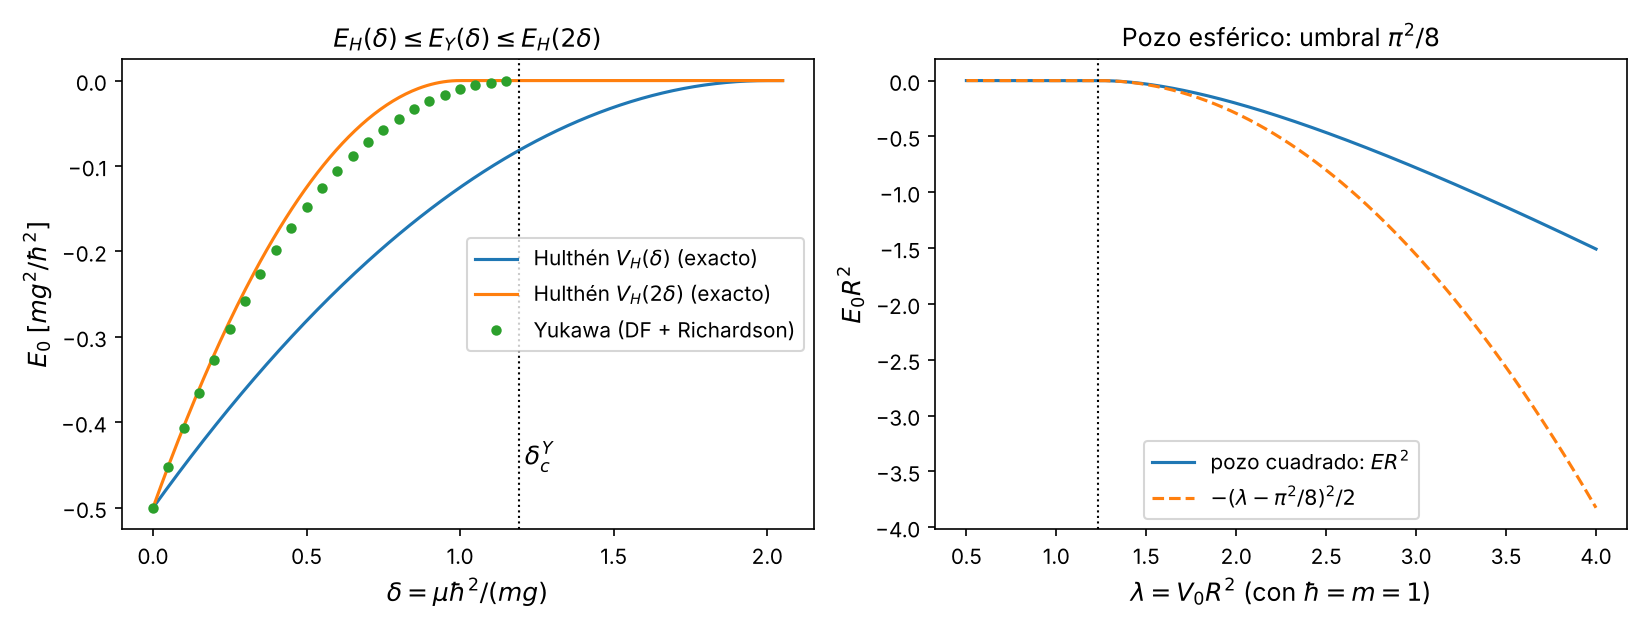
\includegraphics[width=\textwidth]{figuras/00_toy_model.png}
\caption{Izquierda: $E_0$ frente a $\delta$ para Hulthén con $\delta$ y con $2\delta$ (exactos) y para Yukawa (diferencias finitas con Richardson, $R=400$); la línea punteada marca $\dc^Y$. El Yukawa queda entre las dos curvas exactas. Derecha: pozo esférico cuadrado, $E_0R^2$ frente a $\lambda=V_0R^2$, con su ley de umbral cuadrática.}
\label{fig:toy}
\end{figure}

%======================================================================
\section{Adimensionalización de la ecuación radial}
\label{sec:adim}

Script: \texttt{01\_adimensionalizacion.py}.

\subsection{Planteamiento dimensional}

Partícula de masa $m$ en $V(r)=-g\,e^{-\mu r}/r$ con $g>0$ y $\mu\ge0$. Unidades: $[g]=\text{energía}\times\text{longitud}=ML^3T^{-2}$, $[\mu]=L^{-1}$, y $\lambda=1/\mu$ es el alcance. Con $\psi=\frac{u_\ell(r)}{r}Y_{\ell m}$ la ecuación radial es
\begin{equation}
-\frac{\hbar^2}{2m}\,u''(r)+\left[-g\frac{e^{-\mu r}}{r}+\frac{\hbar^2\ell(\ell+1)}{2mr^2}\right]u(r)=E\,u(r).
\label{eq:radial}
\end{equation}
Hay cuatro parámetros dimensionales ($\hbar$, $m$, $g$, $\mu$) y tres dimensiones básicas, así que por el teorema $\Pi$ de Buckingham existe exactamente un grupo adimensional independiente.

\subsection{Escalas naturales}

Igualando la energía cinética típica con la potencial de Coulomb, $\hbar^2/(ma^2)=g/a$:
\[
a=\frac{\hbar^2}{mg}\quad\text{(radio de Bohr generalizado)},\qquad E_H=\frac{g}{a}=\frac{mg^2}{\hbar^2}\quad\text{(Hartree generalizado)}.
\]
Comprobación dimensional: $[a]=\frac{(ML^2T^{-1})^2}{M\cdot ML^3T^{-2}}=L$ y $[E_H]=ML^2T^{-2}$. Para el hidrógeno, $a=a_0\approx0.529\times10^{-10}$~m y $E_H=27.211$~eV.

\subsection{Cambio de variables paso a paso}

Definimos $x=r/a$, $\varepsilon=E/E_H$, $\delta=\mu a=\mu\hbar^2/(mg)$ y $w(x)=u(ax)$.

\begin{enumerate}
\item Derivadas: $\frac{\dd}{\dd r}=\frac1a\frac{\dd}{\dd x}$, así que $u''(r)=w''(x)/a^2$.
\item Cada término: cinético $-\frac{\hbar^2}{2ma^2}w''=-\frac{E_H}{2}w''$; Yukawa $-g\frac{e^{-\mu ax}}{ax}=-E_H\frac{e^{-\delta x}}{x}$; centrífugo $\frac{E_H}{2}\frac{\ell(\ell+1)}{x^2}$; energía $E=\varepsilon E_H$.
\item Sustituyendo en \eqref{eq:radial} y dividiendo entre $-E_H/2$:
\end{enumerate}
\begin{equation}
\boxed{\,w''(x)+\left[\frac{2\,e^{-\delta x}}{x}-\frac{\ell(\ell+1)}{x^2}+2\varepsilon\right]w(x)=0\,}
\label{eq:adim}
\end{equation}
El 2 delante de $e^{-\delta x}/x$ y de $\varepsilon$ sale de dividir entre $E_H/2$; el término centrífugo no lo lleva. Para verificarlo aplicamos con sympy la sustitución literalmente a \eqref{eq:radial}, multiplicamos por $-2/E_H$ y restamos \eqref{eq:adim}: la diferencia es exactamente cero. La ecuación \eqref{eq:adim} es la de unidades atómicas $\hbar=m=g=1$ con $V=-e^{-\delta x}/x$, así que ``$\hbar=m=g=1$'' y ``distancias en radios de Bohr'' son la misma convención.

\textbf{Consecuencia.} El espectro solo depende de $\delta$: $E_{n\ell}=E_H\,\varepsilon_{n\ell}(\delta)$. El umbral es un número puro $\dc$ y $\mu_c=\dc\,mg/\hbar^2$.

\subsection{Condiciones de frontera}

\textbf{Origen.} $\frac{e^{-\delta x}}{x}=\frac1x-\delta+\frac{\delta^2x}{2}-\dots$, así que la singularidad es $1/x$, más débil que $1/x^2$. Con $w\sim x^s$ el término dominante da $s(s-1)=\ell(\ell+1)$, con raíces $s=\ell+1$ y $s=-\ell$. La regular es $w\sim x^{\ell+1}$, $w(0)=0$. Para $\ell=0$ la raíz $s=0$ daría $\psi\sim1/r$, cuya laplaciana produce $\delta^3(\mathbf r)$, y se descarta. Con más precisión, $w=x-x^2+O(x^3)$: la condición de cúspide de Kato, $w''(0)=-2w'(0)$, que no depende de $\delta$.

\textbf{Infinito.} Para $x\to\infty$ el potencial y el término centrífugo se anulan y $w''\approx-2\varepsilon w$. Con $\varepsilon<0$, $w\sim e^{-\kappa x}$ con $\kappa=\sqrt{-2\varepsilon}$. Para $\delta>0$ no aparece el factor $x^{1/\kappa}$ de Coulomb, porque la cola es de corto alcance.

\textbf{Umbral.} Cuando $\delta\to\dc^-$, $\varepsilon\to0^-$ y $\kappa\to0$: la longitud de decaimiento $1/\kappa$ diverge y el estado se deslocaliza. Ya desde aquí se ve que el tamaño de la caja numérica va a ser crítico.

\subsection{Interpretación física de $\delta$}

\[
\delta=\mu a=\frac{a}{\lambda}=\frac{\text{tamaño del átomo}}{\text{alcance del potencial}}.
\]
Si $\delta\ll1$ el alcance es mucho mayor que la órbita y el electrón ``ve'' Coulomb. Si $\delta\sim1$ el apantallamiento corta el potencial a la escala de la propia órbita y la energía sube hacia cero. Si $\delta>\dc\approx1.19$ el pozo es demasiado corto para retener un estado ligado. Otra lectura: $\delta=\frac{\hbar^2\mu^2/m}{g\mu}$ es el cociente entre la energía cinética de confinar la partícula en la longitud $\lambda$ y la profundidad del potencial a esa distancia. El enlace se pierde cuando confinar cuesta más de lo que atrae el pozo.

\textbf{Ejemplo en un plasma.} Con apantallamiento de Debye del hidrógeno, $\delta=a_0/\lambda_D$: $\lambda_D=1$~nm da $\delta=0.053$ y $\lambda_D=0.1$~nm da $\delta=0.529$. El fundamental desaparece para $\lambda_D\approx a_0/1.1906\approx0.0444$~nm. Este ejemplo solo vale en un plasma débilmente acoplado.

\subsection{Comprobaciones}

\begin{table}[H]
\centering
\small
\begin{tabular}{@{}L{9.5cm}l@{}}
\toprule
\textbf{Comprobación} & \textbf{Resultado}\\
\midrule
\eqref{eq:radial} con $r=ax$, $E=\varepsilon E_H$, $\mu=\delta/a$, por $(-2/E_H)$, menos \eqref{eq:adim} & $0$ (sympy, exacto)\\
Dimensión de $\delta$ & $[\delta]=1$\\
$\delta=0$, $\ell=0$, $w=xe^{-x}$, $\varepsilon=-1/2$: residuo de \eqref{eq:adim} & $0$ (exacto)\\
$\langle x\rangle$ del $1s$ hidrogenoide & $3/2$\\
Raíces indiciales & $s=\ell+1$, $s=-\ell$\\
RK45 con $\delta=0$, $\varepsilon=-1/2$ frente a $xe^{-x}$ en $[0,12]$ & error máximo $3.7\times10^{-7}$\\
$\hbar=1.3$, $m=0.7$, $g=2.1$, $\mu=0.45$: $V$ dimensional frente a $E_H\,V_{\rm adim}$ & $8.9\times10^{-16}$\\
\bottomrule
\end{tabular}
\end{table}

\begin{figure}[H]
\centering
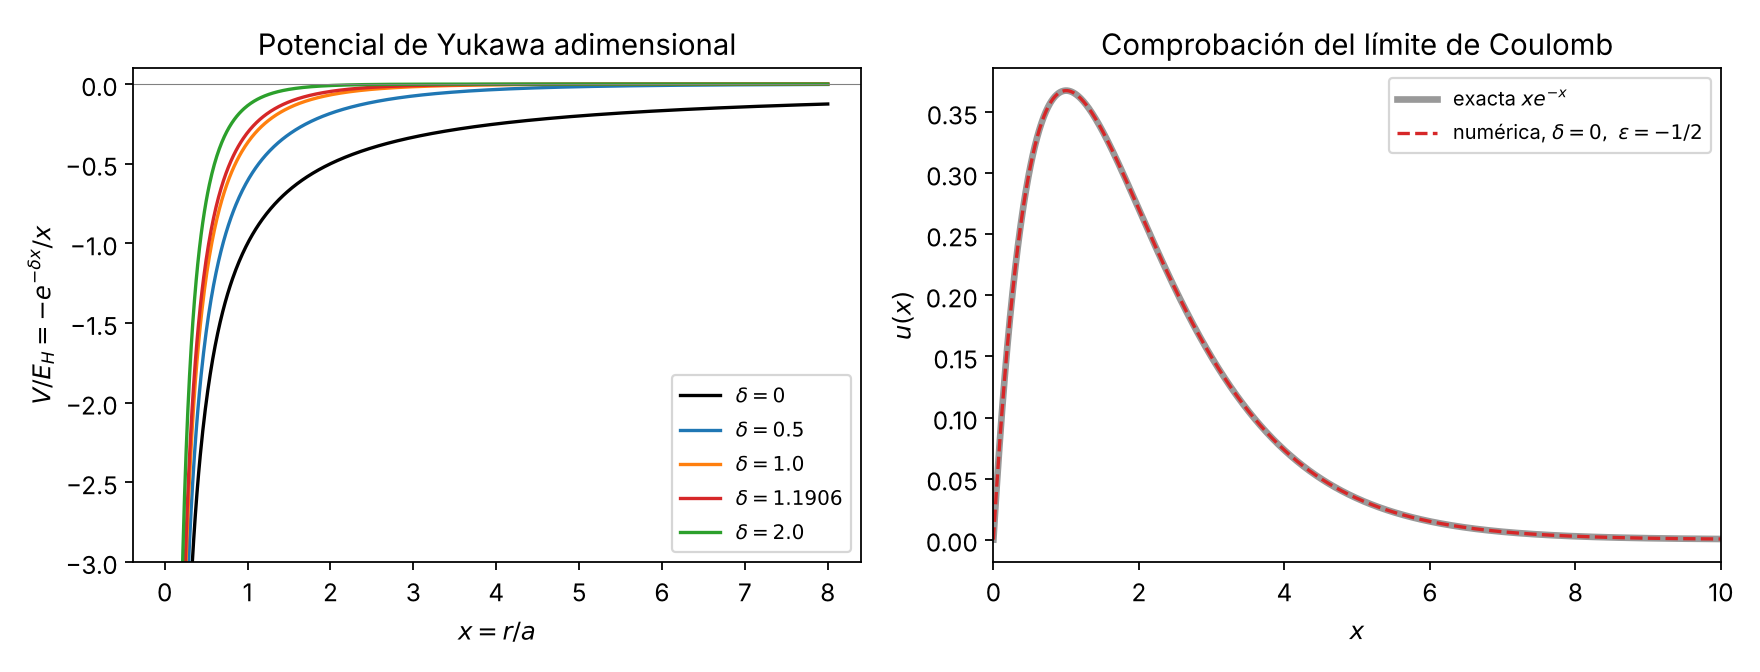
\includegraphics[width=\textwidth]{figuras/01_potencial_adimensional.png}
\caption{Izquierda: $V/E_H=-e^{-\delta x}/x$ para varios $\delta$, incluido $\dc\approx1.1906$. Derecha: solución numérica de \eqref{eq:adim} con $\delta=0$, $\varepsilon=-1/2$ frente a la exacta $xe^{-x}$.}
\end{figure}

%======================================================================
\section{Límite de Coulomb y serie perturbativa de $E_0(\delta)$}
\label{sec:coulomb}

Desde aquí trabajamos en unidades $\hbar=m=g=1$ con $r$ y $E$ adimensionales:
\[
-\tfrac12u''+\Big[\tfrac{\ell(\ell+1)}{2r^2}-\tfrac{e^{-\delta r}}{r}\Big]u=E\,u,\qquad u(0)=0,\quad u(\infty)=0.
\]
Script: \texttt{02\_limite\_coulomb.py}.

\subsection{El límite $\delta\to0$ es el hidrógeno}

Para todo $r$ fijo $e^{-\delta r}\to1$, así que $V\to-1/r$ y $E_n=-1/(2n^2)$; en dimensiones, $E_n=-mg^2/(2\hbar^2n^2)$. Para el $1s$ probamos $u_1=2re^{-r}$: $u_1''=2e^{-r}(r-2)$ y
\[
-\tfrac12u_1''-u_1/r=-e^{-r}(r-2)-2e^{-r}=-re^{-r}=-\tfrac12u_1,
\]
así que $E_1=-1/2$. La normalización es $\int_0^\infty4r^2e^{-2r}\dd r=1$. Con sympy comprobamos además que $u_{n0}=re^{-r/n}L^{(1)}_{n-1}(2r/n)$ cumple $E=-1/(2n^2)$ para $n=1,2,3$. Con $\int_0^\infty r^ke^{-2r}\dd r=k!/2^{k+1}$:
\[
\langle r\rangle=\tfrac32,\qquad\langle r^2\rangle=3,\qquad\langle r^3\rangle=\tfrac{15}{2}.
\]

\subsection{Serie perturbativa}

Expandimos el potencial:
\[
V(r)=-\frac1r+\delta-\frac{\delta^2}{2}r+\frac{\delta^3}{6}r^2-\frac{\delta^4}{24}r^3+O(\delta^5),
\]
de modo que $H=H_0+W$ con $W=\delta-\tfrac{\delta^2}{2}r+\tfrac{\delta^3}{6}r^2-\tfrac{\delta^4}{24}r^3+\dots$

\textbf{Primer orden.} Con los momentos de arriba,
\[
\langle W\rangle=\delta-\frac{\delta^2}{2}\cdot\frac32+\frac{\delta^3}{6}\cdot3-\frac{\delta^4}{24}\cdot\frac{15}{2}=\delta-\frac34\delta^2+\frac12\delta^3-\frac5{16}\delta^4.
\]

\textbf{Segundo orden.} El término $\delta$ es una constante: desplaza todos los niveles por igual y no mezcla estados, así que no contribuye a segundo orden. La primera contribución es la de $W_2=-\tfrac{\delta^2}{2}r$, que entra a orden $\delta^4$. La calculamos exactamente con el método de Dalgarno y Lewis: buscamos $F(r)$ con $[F,H_0]u_1=(W_2-\langle W_2\rangle)u_1$, es decir $(H_0-E_1)(Fu_1)=-(W_2-\langle W_2\rangle)u_1$. Con el ansatz $F=a_0+a_1r+a_2r^2$ sympy da $a_1=0$, $a_2=\tfrac14$ y deja $a_0$ libre, porque una constante por $u_1$ resuelve la ecuación homogénea. Fijamos $a_0=-\tfrac34$ ortogonalizando ($\langle F\rangle_{1s}=0$); no afecta a la energía. Así $F=\tfrac{r^2}{4}-\tfrac34$ y
\[
E^{(2)}[W_2]=\langle(W_2-\langle W_2\rangle)F\rangle=-\tfrac38\,\delta^4 .
\]
\textbf{Resultado:}
\[
\boxed{E_0(\delta)=-\frac12+\delta-\frac34\delta^2+\frac12\delta^3-\frac{11}{16}\delta^4+O(\delta^5)}
\qquad\left(-\tfrac{11}{16}=-\tfrac{5}{16}-\tfrac38\right).
\]
A primer orden el apantallamiento solo sube la energía en $\delta$ (en dimensiones, $g\mu$), porque equivale a sumar la constante $+\delta$ al potencial donde $\delta r\ll1$, que es donde vive el orbital. El término $-\tfrac34\delta^2=-\tfrac{\delta^2}{2}\langle r\rangle$ refleja el tamaño finito del orbital.

\subsection{Verificación numérica}

Diferencias finitas de segundo orden en $(0,60]$ con $u(0)=u(60)=0$, autovalor más bajo con \texttt{eigsh} (shift-invert), pasos $h=0.004$ y $0.002$ y extrapolación de Richardson $E=(4E_{h/2}-E_h)/3$. Para $\delta=0$ reproduce $-0.5$ con error $\sim10^{-11}$.

\begin{table}[H]
\centering
\small
\caption{$E_0(\delta)$ numérico frente a la serie truncada a distintos órdenes.}
\begin{tabular}{@{}lllllll@{}}
\toprule
$\delta$ & $E_0$ numérico & orden 1 & orden 2 & orden 3 & orden 4 & $|E_{\rm num}-E_{(2)}|$\\
\midrule
0.000 & $-0.50000000$ & $-0.500000$ & $-0.50000000$ & $-0.50000000$ & $-0.50000000$ & $7\times10^{-12}$\\
0.005 & $-0.49501869$ & $-0.495000$ & $-0.49501875$ & $-0.49501869$ & $-0.49501869$ & $6.2\times10^{-8}$\\
0.010 & $-0.49007451$ & $-0.490000$ & $-0.49007500$ & $-0.49007450$ & $-0.49007451$ & $4.9\times10^{-7}$\\
0.020 & $-0.48029611$ & $-0.480000$ & $-0.48030000$ & $-0.48029600$ & $-0.48029611$ & $3.9\times10^{-6}$\\
0.050 & $-0.45181643$ & $-0.450000$ & $-0.45187500$ & $-0.45181250$ & $-0.45181680$ & $5.9\times10^{-5}$\\
0.100 & $-0.40705803$ & $-0.400000$ & $-0.40750000$ & $-0.40700000$ & $-0.40706875$ & $4.4\times10^{-4}$\\
0.150 & $-0.36546080$ & $-0.350000$ & $-0.36687500$ & $-0.36518750$ & $-0.36553555$ & $1.4\times10^{-3}$\\
0.200 & $-0.32680851$ & $-0.300000$ & $-0.33000000$ & $-0.32600000$ & $-0.32710000$ & $3.2\times10^{-3}$\\
0.300 & $-0.25763859$ & $-0.200000$ & $-0.26750000$ & $-0.25400000$ & $-0.25956875$ & $9.9\times10^{-3}$\\
\bottomrule
\end{tabular}
\end{table}

\begin{itemize}
\item El error de la serie truncada a orden 2 escala como $\approx\tfrac12\delta^3$ (en $\delta=0.01$: $4.9\times10^{-7}\approx0.5\times10^{-6}$), como se espera del término siguiente.
\item Un ajuste polinómico de grado 4 a 12 puntos en $\delta\in[0.002,0.05]$ da $c_0=-0.5000000$, $c_1=0.9999991$, $c_2=-0.74988$, $c_3=0.494$, frente a $-\tfrac12$, $1$, $-\tfrac34$, $\tfrac12$. El $c_4$ ajustado ($-0.54$) está contaminado por órdenes superiores y no es fiable; el coeficiente $-\tfrac{11}{16}$ se confirma porque la columna ``orden 4'' coincide con el numérico a menos de $10^{-8}$ hasta $\delta=0.02$.
\item La serie solo es útil para $\delta\ll1$. En $\delta=0.3$ la serie de orden 2 ya se desvía $9.86\times10^{-3}$ (3.8~\% de $E_0$) y la de orden 4, $1.93\times10^{-3}$ (0.75~\%). No sirve para estimar $\dc\approx1.19$; para eso están las cotas.
\end{itemize}

\begin{figure}[H]
\centering
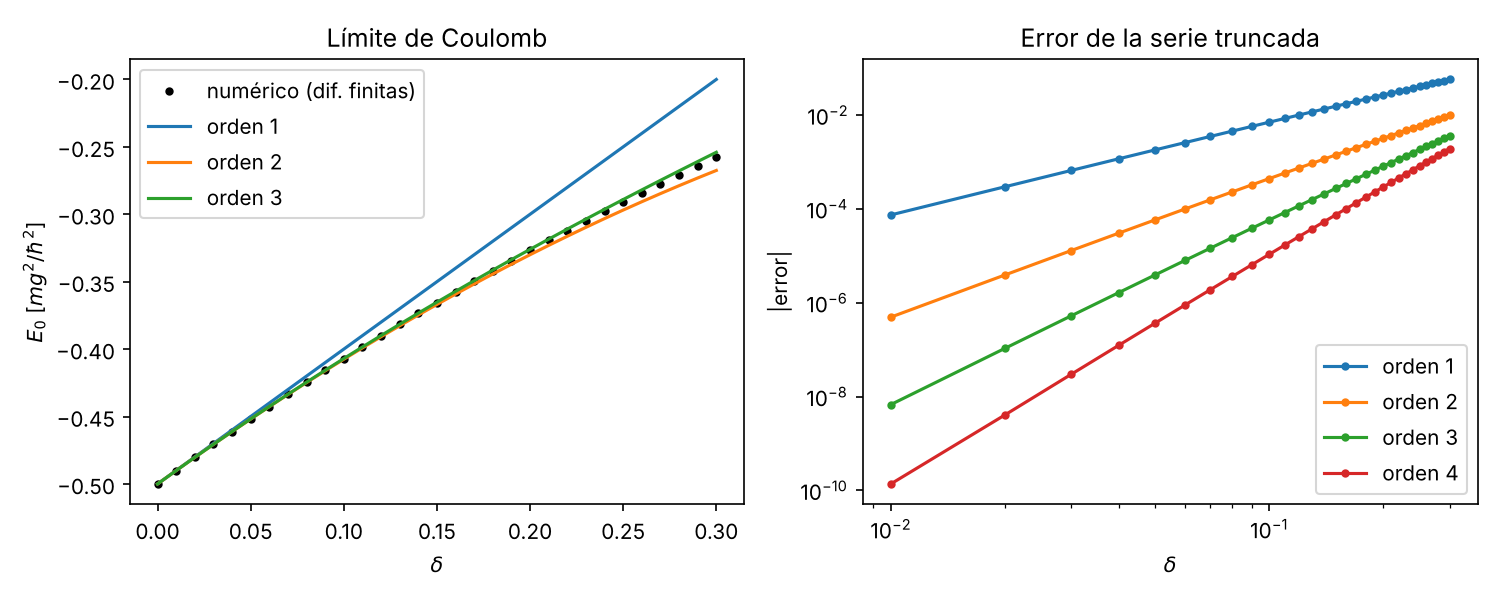
\includegraphics[width=0.95\textwidth]{figuras/02_limite_coulomb.png}
\caption{Izquierda: $E_0(\delta)$ numérico frente a la serie truncada a órdenes 1 a 3. Derecha: error absoluto de la serie truncada a órdenes 1 a 4 en escala log-log; las pendientes son $\approx k+1$.}
\end{figure}

Esto nos deja una prueba de control para la Fase 2: cualquier solucionador debe reproducir $E_0(0)=-0.5$ y la pendiente $\dd E_0/\dd\delta|_0=1$.

%======================================================================
\section{Criterio de estado ligado I: cota inferior por el método variacional}
\label{sec:inferior}

Script: \texttt{03\_cota\_variacional.py}.

\subsection{Idea}

El hamiltoniano adimensional es $H=-\tfrac12\nabla^2-e^{-\delta r}/r$. Por el principio de Rayleigh y Ritz, para cualquier $\psi$ normalizable $E[\psi]=\langle\psi|H|\psi\rangle/\langle\psi|\psi\rangle\ge E_0$. Como el continuo empieza en $E=0$, basta encontrar \emph{una} $\psi$ con $E[\psi]<0$ para asegurar que hay un estado ligado. Así, todo $\delta$ para el que alguna prueba da $E<0$ cumple $\delta<\dc$: el método da \textbf{cotas inferiores de $\dc$}.

Para $\ell=0$ (el $4\pi$ se cancela):
\[
\langle\psi|\psi\rangle=\int_0^\infty\psi^2r^2\dd r,\quad\langle T\rangle=\tfrac12\int_0^\infty(\psi')^2r^2\dd r,\quad\langle V\rangle=-\int_0^\infty\psi^2e^{-\delta r}\,r\,\dd r,
\]
y la integral que usamos todo el tiempo es $\int_0^\infty r^ne^{-sr}\dd r=n!/s^{n+1}$.

\subsection{Prueba hidrogenoide $\psi=e^{-r/b}$}

Norma: $\int_0^\infty r^2e^{-2r/b}\dd r=b^3/4$. Cinética: $\langle T\rangle=\frac{b/8}{b^3/4}=\frac{1}{2b^2}$. Potencial: $-\int_0^\infty re^{-(2/b+\delta)r}\dd r=-\frac{b^2}{(2+\delta b)^2}$, luego $\langle V\rangle=-\frac{4}{b(2+\delta b)^2}$. Entonces
\[
\boxed{E(b,\delta)=\frac{1}{2b^2}-\frac{4}{b\,(2+\delta b)^2}}
\]
(con $\beta=1/b$: $E=\beta^2/2-4\beta^3/(2\beta+\delta)^2$, que es la forma que usamos en la presentación del 5 de octubre). Lo comprobamos con sympy y con una integral numérica en $b=1.7$, $\delta=0.6$: $-0.0849762401910$ por las dos vías. En $\delta=0$, $E=\frac{1}{2b^2}-\frac1b$ tiene mínimo en $b^*=1$ con $E^*=-\tfrac12$: la prueba es exacta para el hidrógeno.

\textbf{Existencia de estado ligado para $\delta<1$.} Como $b>0$, multiplicando por $2b^2(2+\delta b)^2>0$,
\[
E<0\iff(2+\delta b)^2<8b\iff P(b)\equiv\delta^2b^2+(4\delta-8)\,b+4<0 .
\]
$P$ es una parábola convexa con $P(0)=4>0$, que toma valores negativos si y solo si tiene dos raíces reales positivas distintas. Su discriminante es
\[
\Delta=(4\delta-8)^2-16\delta^2=-64(\delta-1).
\]
\begin{itemize}
\item Si $\delta<1$: $\Delta>0$ y las raíces $b_\pm=\frac{2(2-\delta\pm2\sqrt{1-\delta})}{\delta^2}$ son positivas (producto $4/\delta^2$, suma $(8-4\delta)/\delta^2$). Para todo $b\in(b_-,b_+)$, $E<0$: \textbf{hay estado ligado}.
\item Si $\delta=1$: $P(b)=(b-2)^2\ge0$; el mínimo toca cero en $b=2$, con $E(2,1)=0$.
\item Si $\delta>1$: $P>0$ siempre; el ínfimo de $E$ es $0^+$ cuando $b\to\infty$ (la prueba se dispersa al continuo).
\end{itemize}
\[
\boxed{\dc\ge1}
\]

\textbf{¿Por qué exactamente 1?} Con $x=\delta b$ la condición $E<0$ es $\delta<g_1(x)=\frac{8x}{(x+2)^2}$, y $g_1'(x)=\frac{8(2-x)}{(x+2)^3}=0$ da $x=2$, $g_1(2)=1$. La función $e^{-r/b}$ tiene una sola escala; el mejor compromiso se da cuando $b=2/\delta$, es decir cuando la longitud de decaimiento de $\psi^2$ coincide con el alcance. El número 1 es una propiedad de la familia de prueba, no del potencial. La función de onda real cerca del umbral tiene \emph{dos} escalas (un núcleo de tamaño $\sim1$ y una cola $e^{-\kappa r}$ con $\kappa\to0$), que un solo exponencial no puede representar; por eso la cota no es óptima.

\textbf{Control para $\delta$ pequeño.} De $\partial_bE=0$ se obtiene por serie $b^*=1+\tfrac34\delta^2-\delta^3+\dots$ y $E_{\min}=-\tfrac12+\delta-\tfrac34\delta^2+\tfrac12\delta^3+O(\delta^4)$, que coincide con la teoría de perturbaciones de primer orden de la sección~\ref{sec:coulomb}.

\begin{table}[H]
\centering
\small
\begin{tabular}{@{}lll@{}}
\toprule
$\delta$ & $b^*$ & $E^{(1)}_{\min}$\\
\midrule
0 & 1.0000 & $-0.500000$\\
0.5 & 1.1448 & $-0.146509$\\
0.9 & 1.6243 & $-0.015969$\\
0.99 & 1.9438 & $-0.001287$\\
1 & 2.0000 & 0 (mínimo marginal: raíz doble de $P$)\\
$>1$ & $b\to\infty$ & ínfimo $0^+$, no alcanzado\\
\bottomrule
\end{tabular}
\end{table}

\subsection{Prueba con un polinomio: $\psi=(1+cr)e^{-r/b}$}

Con sympy:
\[
N=\tfrac{b^3}{4}(1+3bc+3b^2c^2),\qquad\tfrac12\!\int\!\psi'^2r^2\,\dd r=\tfrac b8(1+bc+b^2c^2),
\]
\[
-\!\int\!\psi^2e^{-\delta r}r\,\dd r=-\frac{b^2\left[(2+\delta b)^2+4bc(2+\delta b)+6b^2c^2\right]}{(2+\delta b)^4}.
\]
Con $x=\delta b$ y $t=cb$, $E<0\iff\delta<g_2(x,t)=\frac{8x\left[(x+2)^2+4t(x+2)+6t^2\right]}{(x+2)^4(1+t+t^2)}$. Maximizando numéricamente (Nelder-Mead desde 16 puntos) sale $\max g_2=1.000000$ en $x=2$, $t=0$: \textbf{no mejora la cota}. La razón es que $\partial_cE|_{c=0}$ es idéntico, salvo un factor $b^2$, a $\partial_bE^{(1)}$: añadir $cr\,e^{-r/b}$ es a primer orden lo mismo que cambiar $b$. En $x=2$, $g_2(2,t)=1-\frac{5t^2/8}{1+t+t^2}\le1$. En 34 valores de $\delta\in[0,0.99]$ el script da $\max|E^{(2)}_{\min}-E^{(1)}_{\min}|=9.8\times10^{-15}$ y $|t^*|\le2.3\times10^{-5}$. Es un resultado negativo pero útil: \emph{la mejora tiene que venir de añadir escalas, no polinomios}.

\subsection{Combinación de exponenciales (Ritz lineal)}

Tomamos $u(r)=r\psi=\sum_{i=1}^Nc_i\,r\,e^{-a_ir}$ con $a_i=a_1\rho^{i-1}$. Con $s=a_i+a_j$,
\[
S_{ij}=\frac{2}{s^3},\qquad T_{ij}=\frac{a_ia_j}{s^3},\qquad V_{ij}=-\frac{1}{(s+\delta)^2}.
\]
Resolvemos $(T+V)\mathbf c=E\,S\,\mathbf c$ (con ortogonalización canónica para evitar dependencia lineal), minimizamos el menor autovalor en $(a_1,\rho)$ y buscamos con \texttt{brentq} el $\delta$ donde $E_{\min}=0$. Cada autovalor es cota superior de $E_0$ (teorema de Hylleraas-Undheim y MacDonald), así que $E_{\min}<0$ implica ligado. Control: con $N=10$ y $\delta=0$ sale $E=-0.5000000000000$.

\begin{table}[H]
\centering
\small
\caption{Cotas inferiores de $\dc$ con bases cada vez más ricas.}
\begin{tabular}{@{}ll@{}}
\toprule
\textbf{Prueba} & \textbf{Cota inferior de $\dc$}\\
\midrule
$e^{-r/b}$ & 1.000000 (analítica)\\
$(1+cr)e^{-r/b}$ & 1.000000\\
2 exponenciales & 1.147636\\
4 exponenciales & 1.184635\\
8 exponenciales & 1.190195\\
12 exponenciales & \textbf{1.190550}\\
16 exponenciales & 1.190546 (la base geométrica restringida ya no mejora)\\
\bottomrule
\end{tabular}
\end{table}

Con solo \emph{dos} exponenciales (núcleo y cola) la cota sube a 1.1476. La mejor que obtuvimos es
\[
\boxed{\dc\ge1.19055}
\]
que queda por debajo, como debe, del valor de referencia $1.19061242106$ y del nuestro ($1.1906124211$, sección~\ref{sec:numerico}).

\begin{table}[H]
\centering
\small
\begin{tabular}{@{}llll@{}}
\toprule
$\delta$ & $e^{-r/b}$ & $(1+cr)e^{-r/b}$ & 12 exponenciales\\
\midrule
0 & $-0.500000$ & $-0.500000$ & $-0.500000$\\
0.2 & $-0.326729$ & $-0.326729$ & $-0.326809$\\
0.4 & $-0.197576$ & $-0.197576$ & $-0.198376$\\
0.6 & $-0.103354$ & $-0.103354$ & $-0.106136$\\
0.8 & $-0.038471$ & $-0.038471$ & $-0.044704$\\
1.0 & 0 & 0 & $-0.010286$\\
1.1 & 0 & 0 & $-0.002287$\\
\bottomrule
\end{tabular}
\end{table}

\begin{figure}[H]
\centering
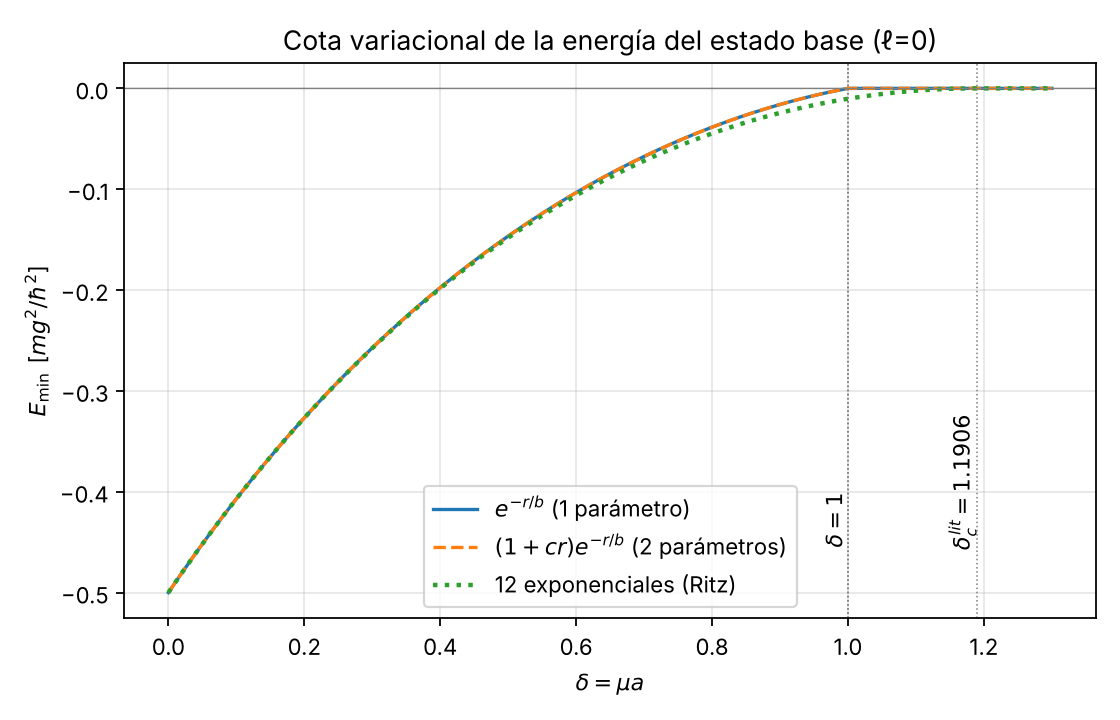
\includegraphics[width=0.75\textwidth]{figuras/03_Emin_vs_delta.png}
\caption{Energía variacional mínima frente a $\delta$. La prueba hidrogenoide llega a cero en $\delta=1$; la base de exponenciales sigue ligada hasta $\delta\approx1.1906$, donde $E\to0^-$ de forma aproximadamente cuadrática, como corresponde a un umbral de onda $s$.}
\end{figure}

Como contraste independiente, diferencias finitas con 40\,000 nodos y $R=400$ dan $E(\delta=1.1)=-0.002285$ frente a $-0.002287$ de Ritz, que es cota superior de $E_0$, como debe ser.

%======================================================================
\section{Criterio de estado ligado II: cotas superiores}
\label{sec:superior}

Script: \texttt{04\_cota\_bargmann.py}.

\subsection{Planteamiento}

En unidades de Bohr la ecuación radial es
\[
u''=\Big[-U(x)+\frac{\ell(\ell+1)}{x^2}-2E\Big]u,\qquad U(x)\equiv\frac{2m}{\hbar^2}|V|\,a^2=\frac{2\,e^{-\delta x}}{x}.
\]
\textbf{Cuidado con el factor 2.} En unidades físicas $\frac{2m}{\hbar^2}\int_0^\infty r|V|\,\dd r=\frac{2mg}{\hbar^2}\,a\int_0^\infty e^{-\delta x}\dd x=\frac{2}{\delta}$, porque $mga/\hbar^2=1$. El 2 viene de $2m/\hbar^2$ y no se puede omitir. Lo comprobamos por otro lado: sin él saldría $1/\delta$ y la ``cota'' $\dc\le1$, que es falsa, porque en $\delta=1$ todavía hay estado ligado ($E_0=-0.0103$).

\subsection{Teorema de Bargmann (1952)}

Para un potencial central con $\int_0^\infty r|V|\,\dd r<\infty$, el número $n_\ell$ de estados ligados con momento angular $\ell$ cumple
\[
n_\ell<\frac{1}{2\ell+1}\,\frac{2m}{\hbar^2}\int_0^\infty r\,|V(r)|\,\dd r .
\]
Para Yukawa con $\ell=0$: $\int_0^\infty xU\,\dd x=2\int_0^\infty e^{-\delta x}\dd x=2/\delta$, luego $n_0<2/\delta$ (y en general $n_\ell<\frac{2}{(2\ell+1)\delta}$). Si $\delta\ge2$, $n_0<1$ y por tanto $n_0=0$: \textbf{no hay estado ligado para $\delta\ge2$}, así que $\dc\le2$. Sympy da \texttt{2/delta}; numéricamente, en $\delta=0.7$ la cuadratura da $2.857142857$, igual a $2/0.7$.

\subsection{Cota de Calogero (1965)}

Para potenciales atractivos no decrecientes (H7, que Yukawa cumple), $n_0<\frac{2}{\pi}\int_0^\infty\sqrt{U}\,\dd x$. Aquí $\sqrt U=\sqrt2\,x^{-1/2}e^{-\delta x/2}$ (el exponente se divide entre 2) y $\int_0^\infty x^{-1/2}e^{-\delta x/2}\dd x=\sqrt{2\pi/\delta}$, así que $n_0<\frac{4}{\sqrt{\pi\delta}}$, que es menor que 1 si $\delta\ge16/\pi\approx5.093$. Es \textbf{mucho peor que Bargmann} para este potencial, porque la singularidad $1/x$ hace grande $\int\sqrt U$ cerca del origen.

\subsection{Cota de Schwinger (Birman-Schwinger, 1961)}

A energía cero, que exista un estado $s$ ligado equivale a que el operador integral simétrico
\[
K(x,y)=\sqrt{U(x)}\;\min(x,y)\;\sqrt{U(y)}
\]
tenga un autovalor $\ge1$ ($\min(x,y)$ es la función de Green de $-\dd^2/\dd x^2$ con $u(0)=0$), y $n_0$ es el número de autovalores $\ge1$. Como $\lambda_{\max}^p\le\Tr K^p$, se obtiene la familia de cotas $n_0\le\Tr K^p$. Con $p=1$ se recupera exactamente Bargmann. Con $p=2$:
\[
\Tr K^2=\int_0^\infty\!\!\int_0^\infty U(x)U(y)\min(x,y)^2\,\dd x\,\dd y=8\int_0^\infty\frac{e^{-\delta y}}{y}\Big[\int_0^yxe^{-\delta x}\dd x\Big]\dd y .
\]
\begin{enumerate}
\item $\int_0^yxe^{-\delta x}\dd x=\frac{1-(1+\delta y)e^{-\delta y}}{\delta^2}$.
\item $\Tr K^2=\frac{8}{\delta^2}\Big[\int_0^\infty\frac{e^{-\delta y}-e^{-2\delta y}}{y}\dd y-\delta\int_0^\infty e^{-2\delta y}\dd y\Big]$.
\item Por Frullani la primera integral es $\ln2$, y la segunda da $\tfrac12$.
\item $\Tr K^2=\dfrac{4(2\ln2-1)}{\delta^2}$.
\item No hay estado ligado si $\Tr K^2<1$: $\dc\le2\sqrt{2\ln2-1}\approx1.24305$.
\end{enumerate}
Sympy da exactamente \texttt{4*(-1+2*log(2))/delta**2}; la discretización numérica de $K$ con 1500 nodos de Gauss-Legendre da $1.243053$. Con potencias mayores (numérico): $\Tr K^3=1\Rightarrow\delta\le1.19838$ y $\Tr K^4=1\Rightarrow\delta\le1.19205$. En el límite, $\lambda_{\max}(K)=1$ da $\dc=1.1906134$; la diferencia de $10^{-6}$ con el disparo es error de discretización de $K$.

\subsection{Comparación}

\begin{table}[H]
\centering
\small
\caption{Cotas superiores de $\dc$.}
\begin{tabular}{@{}llll@{}}
\toprule
\textbf{Cota} & \textbf{Expresión para $n_0$} & $\delta_{\max}$ & \textbf{Exceso sobre $\dc$}\\
\midrule
Calogero & $4/\sqrt{\pi\delta}$ & $16/\pi=5.0930$ & $+328~\%$\\
Bargmann ($\Tr K$) & $2/\delta$ & $2$ & $+68~\%$\\
Schwinger ($\Tr K^2$) & $4(2\ln2-1)/\delta^2$ & $1.24305$ & $+4.4~\%$\\
$\Tr K^3$ (numérico) & --- & $1.1984$ & $+0.65~\%$\\
$\Tr K^4$ (numérico) & --- & $1.1920$ & $+0.12~\%$\\
Exacto ($\lambda_{\max}(K)=1$, disparo) & --- & $1.19061$ & $0$\\
\bottomrule
\end{tabular}
\end{table}

De las cotas cerradas, la de Schwinger es la más ajustada; la de Bargmann es la más simple y la de Calogero no sirve aquí. Junto con la cota inferior de Ritz,
\[
\boxed{1.19055\le\dc\le1.24305}
\]
y el intervalo elemental, con la prueba $e^{-r/b}$ y Bargmann (o con Hulthén), es $1\le\dc\le2$.

\begin{figure}[H]
\centering
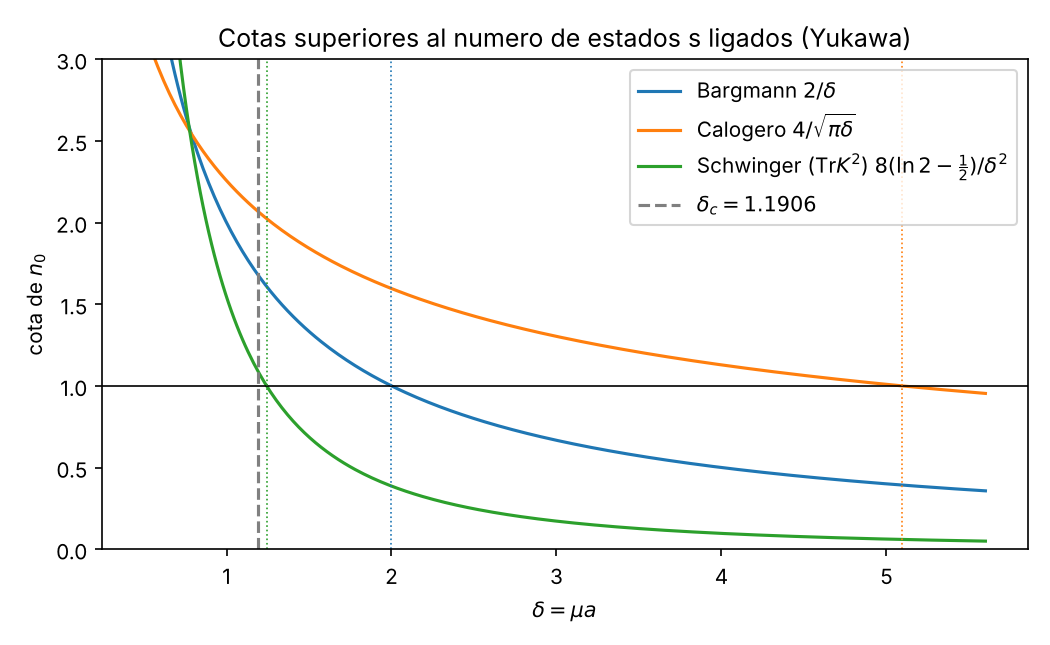
\includegraphics[width=0.72\textwidth]{figuras/04_cotas_superiores.png}
\caption{Cotas de $n_0$ frente a $\delta$; el cruce con $n_0=1$ marca cada $\delta_{\max}$ (líneas punteadas en $1.243$, $2$ y $16/\pi\approx5.09$). La curva de Calogero es $4/\sqrt{\pi\delta}$, que vale $2.257$ en $\delta=1$.}
\end{figure}

%======================================================================
\section{Recálculo independiente del umbral}
\label{sec:numerico}

El resultado principal, $\dc$, lo recalculamos por caminos que no comparten nada con las cotas analíticas. Esto no es todavía la Fase 2; es una validación y la referencia contra la que se medirá la integral de camino. Script: \texttt{05\_referencia\_numerica.py}. Ecuación: $-\tfrac12u''-\frac{e^{-\delta r}}{r}u=Eu$, $u(0)=u(\infty)=0$.

\subsection{Método A: diferencias finitas con Richardson}

Caja $[0,R]$ con $u(R)=0$, malla uniforme $r_j=jh$. Con $u''\approx(u_{j+1}-2u_j+u_{j-1})/h^2$ queda la matriz tridiagonal $H_{jj}=\frac{1}{h^2}-\frac{e^{-\delta r_j}}{r_j}$, $H_{j,j\pm1}=-\frac{1}{2h^2}$, cuyo menor autovalor es $E_0$. Como $E_h=E+Ch^2+\dots$, con $h$ y $h/2$ se extrapola $E\approx(4E_{h/2}-E_h)/3$. Para que el error de caja sea despreciable ($\sim e^{-50}$) tomamos $R=\max(60,25/\kappa)$ y $h=1/40$.

\begin{table}[H]
\centering
\small
\begin{tabular}{@{}llllll@{}}
\toprule
$\delta$ & $R$ & $N$ & $E_0$ & $\langle r\rangle$ & $|E_h-E_{h/2}|$\\
\midrule
0.0 & 60 & 2400 & $-0.499999994$ & 1.50000 & $5.9\times10^{-5}$\\
0.2 & 60 & 2400 & $-0.326808505$ & 1.54972 & $5.7\times10^{-5}$\\
0.4 & 60 & 2400 & $-0.198376077$ & 1.69137 & $5.1\times10^{-5}$\\
0.6 & 60 & 2400 & $-0.106135901$ & 1.96686 & $4.3\times10^{-5}$\\
0.8 & 84 & 3344 & $-0.044704298$ & 2.54916 & $3.2\times10^{-5}$\\
1.0 & 174 & 6972 & $-0.010285784$ & 4.36670 & $1.8\times10^{-5}$\\
1.1 & 370 & 14795 & $-0.002287239$ & 8.27764 & $8.8\times10^{-6}$\\
\bottomrule
\end{tabular}
\end{table}

En $\delta=0$ se recupera $-1/2$ con error $6\times10^{-9}$ y $\langle r\rangle=3/2$. Además $E_0(1)=-0.01029<0$: en $\delta=1$ todavía hay estado ligado, como dice la cota $\dc\ge1$.

\subsection{Método B: Numerov con disparo en malla logarítmica}

Con $r=e^x$ y $u=\sqrt r\,y$ se tiene $u''=e^{-3x/2}(y''-y/4)$ y la ecuación queda $y''=f(x)\,y$ con $f=\tfrac14+2r^2(V-E)$, que tiene la forma de Numerov ($c_i=1-\tfrac{h^2}{12}f_i$, $y_{i+1}=[(12-10c_i)y_i-c_{i-1}y_{i-1}]/c_{i+1}$). Arrancamos con $u\simeq r(1-r)$ (Frobenius) en $r_{\min}=10^{-6}$, con 40\,000 nodos hasta $R=\max(40,30/\kappa)$, y buscamos con \texttt{brentq} el $E$ que anula $y(R)$.

\begin{table}[H]
\centering
\small
\begin{tabular}{@{}llll@{}}
\toprule
$\delta$ & $E_0$ Numerov & $E_0$ DF + Richardson & Diferencia\\
\midrule
0.0 & $-0.4999999999$ & $-0.4999999939$ & $6.0\times10^{-9}$\\
0.5 & $-0.1481170219$ & $-0.1481170192$ & $2.7\times10^{-9}$\\
1.0 & $-0.0102857900$ & $-0.0102857842$ & $5.7\times10^{-9}$\\
\bottomrule
\end{tabular}
\end{table}

Dos discretizaciones distintas concuerdan en $\sim10^{-8}$.

\subsection{Método C: condición de umbral a energía cero}

En el umbral el estado llega a $E=0$, donde $u''=-\frac{2e^{-\delta r}}{r}u$. Para $r\gg1/\delta$ el potencial es despreciable y $u\simeq A+Br$. Con $\delta<\dc$ el pozo ya ``giró'' la función (hay estado ligado, $B<0$); con $\delta>\dc$, $B>0$. El umbral es exactamente $B(\dc)=0$, es decir $u'(\infty)=0$: una resonancia de energía cero, con longitud de dispersión infinita. Integramos con \texttt{solve\_ivp} (DOP853, $\text{rtol}=10^{-13}$) desde $r=10^{-8}$ con $u=r$, $u'=1$, y resolvemos $u'(R;\delta)=0$ con \texttt{brentq}.

\begin{table}[H]
\centering
\small
\begin{tabular}{@{}lll@{}}
\toprule
$R$ & $\dc$ & $\dc-1.19061242106$\\
\midrule
200 & 1.1906124211 & $6\times10^{-13}$\\
400 & 1.1906124211 & $6\times10^{-13}$\\
800 & 1.1906124211 & $6\times10^{-13}$\\
\bottomrule
\end{tabular}
\end{table}

El resultado no depende de $R$, así que el error de caja es nulo a esta precisión. \textbf{$\dc=1.1906124211$ coincide con el valor de referencia $1.19061242106$ dentro de $6\times10^{-13}$.} Este acuerdo respalda el número de forma independiente, aunque no verifica la cita (sección~\ref{sec:fuentes}). Una sutileza: el signo $B<0$ para $\delta<\dc$ vale entre $\dc$ y el umbral del segundo estado $s$; como buscamos el cero más cercano en un intervalo que encierra a $\dc$, no nos afecta.

\subsection{Método D: extrapolación de $\kappa\to0$}

Cerca del umbral, para $\ell=0$, $\kappa=\sqrt{-2E_0}$ se anula linealmente, $\kappa\simeq c(\dc-\delta)$, y por eso $E_0\simeq-\tfrac{c^2}{2}(\dc-\delta)^2$ llega a cero tangencialmente. Ajustamos un polinomio a $\kappa(\delta)$ en 11 puntos de $[1.05,1.15]$ (método A con $R=\min(40/\kappa,8000)$, $h=1/20$):

\begin{table}[H]
\centering
\small
\begin{tabular}{@{}lllllll@{}}
\toprule
$\delta$ & 1.05 & 1.07 & 1.09 & 1.11 & 1.13 & 1.15\\
\midrule
$\kappa$ & 0.105375 & 0.090241 & 0.075158 & 0.060122 & 0.045134 & 0.030193\\
\bottomrule
\end{tabular}
\end{table}

La pendiente secante es $\approx-0.752$, casi constante. El ajuste de grado 2 da $\dc=1.190618$ ($+5.7\times10^{-6}$) y el de grado 3, $1.190605$ ($-7.2\times10^{-6}$): $\dc=1.19061\pm0.00001$, de acuerdo con el método C. Ojo: la pendiente secante sobreestima el coeficiente asintótico; más cerca del umbral $\kappa/(\dc-\delta)$ baja y extrapola a $c\approx0.741$ (sección~\ref{sec:limites}).

\subsection{Tamaño del estado}

$\langle r\rangle$ crece de 1.5 ($\delta=0$) a 4.37 ($\delta=1$), 17.97 ($\delta=1.151$) y 33.5 ($\delta=1.170$): diverge como $\langle r\rangle\sim1/(2\kappa)\propto(\dc-\delta)^{-1}$. El estado ``se escapa'' al acercarse al umbral. En $\delta=1.170$, $E_0=-1.1685\times10^{-4}$ da $1/(2\kappa)=32.7$, cerca del 33.5 medido.

\begin{figure}[H]
\centering
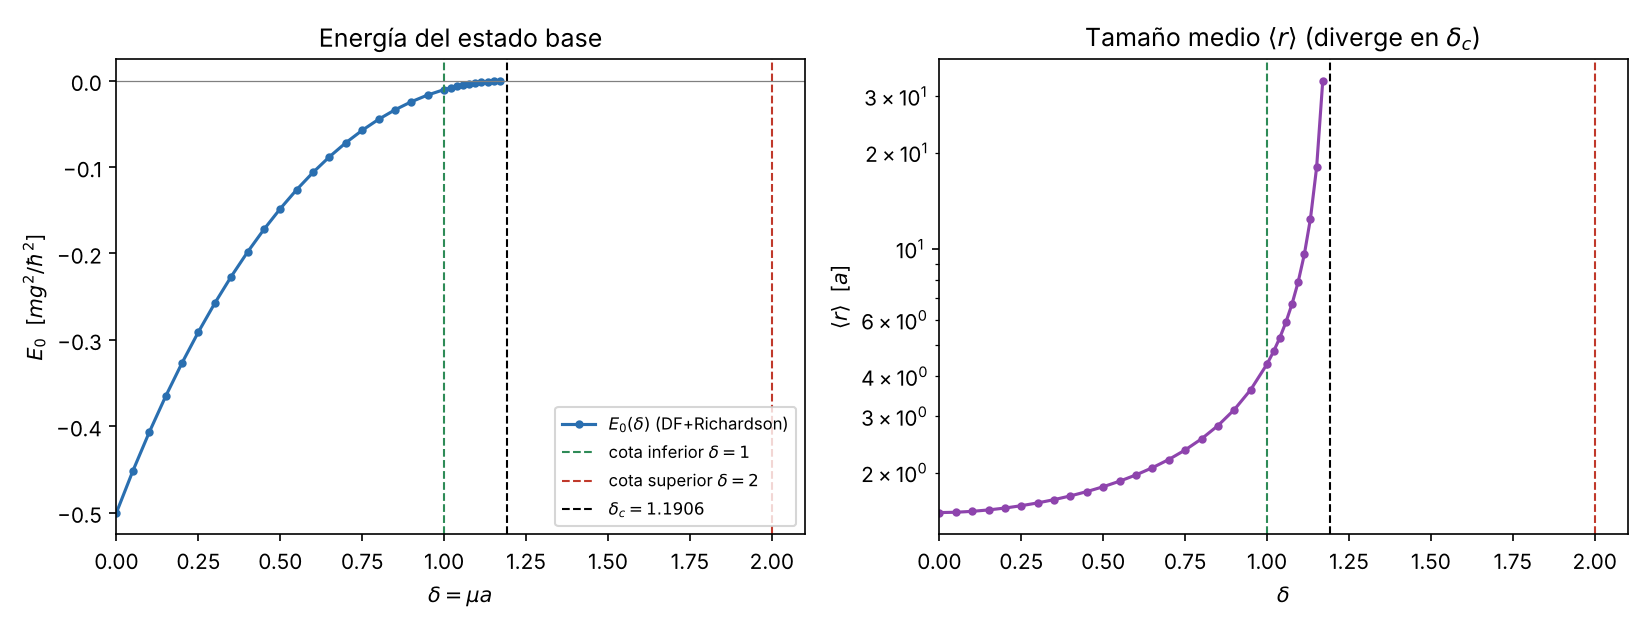
\includegraphics[width=\textwidth]{figuras/05_E0_r_vs_delta.png}
\caption{$E_0(\delta)$ y $\langle r\rangle(\delta)$ con el método A. La energía llega a cero de forma cuadrática en $\dc$ y el radio medio diverge.}
\end{figure}

\subsection{Resumen del umbral}

\begin{table}[H]
\centering
\small
\begin{tabular}{@{}lll@{}}
\toprule
\textbf{Cantidad} & \textbf{Valor} & \textbf{Fuente}\\
\midrule
Cota inferior elemental (prueba $e^{-r/b}$) & $\dc\ge1$ & sección~\ref{sec:inferior}\\
Mejor cota inferior (Ritz, 12 exponenciales) & $\dc\ge1.19055$ & sección~\ref{sec:inferior}\\
Método C (energía cero) & $1.1906124211$ & esta sección\\
Método D (extrapolación de $\kappa$) & $1.19061\pm10^{-5}$ & esta sección\\
Disparo en otros scripts (00 y 04) & $1.1906124211$ & secciones~\ref{sec:toy}, \ref{sec:superior}\\
Núcleo de Birman-Schwinger, $\lambda_{\max}(K)=1$ & $1.1906134$ & sección~\ref{sec:superior}\\
Referencia de alta precisión & $1.19061242106$ & Gebremedhin y Weatherford 2023\\
Literatura, primer cálculo & $\approx1.19$ & Rogers et al.\ 1970\\
Mejor cota superior (Schwinger) & $\dc\le1.24305$ & sección~\ref{sec:superior}\\
Cota superior elemental (Bargmann) & $\dc\le2$ & sección~\ref{sec:superior}\\
\bottomrule
\end{tabular}
\end{table}

$1.19055<1.1906124<1.24305$, y por tanto también $1<\dc<2$. Las cotas elementales están a un 16~\% (variacional) y un 68~\% (Bargmann) del valor numérico; la mejor cota inferior queda $6\times10^{-5}$ por debajo y la mejor superior un 4.4~\% por encima.

\textbf{Límite de la independencia.} Los métodos A a D y la tabla de la acción de pares de la Fase 2 comparten la discretización por diferencias finitas en algunos pasos. Por eso la referencia externa es la literatura, con la salvedad de que el valor de diez cifras lo tomamos de una cita secundaria, y la advertencia sobre circularidad la retomamos en la sección~\ref{sec:plan}.

%======================================================================
\section{Límites físicos que debe cumplir el algoritmo}
\label{sec:limites}

Este es el requisito explícito de la guía para la Fase 1: ``pedir a la IA una lista de límites físicos que el algoritmo debe cumplir y verificarla''. El algoritmo es doble: el solucionador radial y la formulación en tiempo imaginario que se construirá en la Fase 2. Pedimos la lista, \emph{la guardamos antes de verificar nada} para que la verificación no la contaminara, y la comprobamos ítem por ítem. Script: \texttt{07\_limites\_fisicos.py}.

\subsection{Consulta}

Seguimos el formato de ``consulta de derivación'' de la guía: pregunta delimitada, hipótesis explícitas y sin pedir código. El 12 de octubre le enviamos a Claude:

\begin{prompt}
Para la ecuación radial $-\tfrac12u''-e^{-\delta r}u/r=Eu$ en unidades $\hbar=m=g=1$, con $\ell=0$, $u(0)=0$ y $u(\infty)=0$, dame una lista numerada de límites físicos y propiedades exactas que deben cumplir (a) un solucionador radial en caja finita y (b) una formulación en tiempo imaginario (integral de camino) para el estado fundamental. Para cada ítem indica: el enunciado, sus hipótesis, si es una condición necesaria o una prueba de falsación, y cómo se comprobaría. No escribas código. Indica explícitamente si el peso que se pretende muestrear es real, positivo y normalizable.
\end{prompt}

\subsection{Respuesta de la IA (sin editar en contenido)}

N indica condición necesaria (si falla, el algoritmo está mal); F indica prueba de falsación (diseñada para detectar un artefacto que podría pasar por resultado).

\begin{enumerate}[label=\textbf{L\arabic*.},leftmargin=2.2em]
\item \textbf{Escalamiento (N).} $E_0=(mg^2/\hbar^2)\,\varepsilon(\delta)$; cambiar $m$ y $g$ a $\delta$ fijo no debe cambiar $\varepsilon$.
\item \textbf{Coulomb (N).} En $\delta=0$: $E_0=-1/2$, $\langle r\rangle=3/2$, $\langle r^2\rangle=3$.
\item \textbf{Serie (N).} $E_0=-\tfrac12+\delta-\tfrac34\delta^2+\tfrac12\delta^3-\tfrac{11}{16}\delta^4+O(\delta^5)$.
\item \textbf{Cotas (N).} $-\tfrac12\le E_0(\delta)\le-\tfrac12+\delta$, porque $-1/r\le-e^{-\delta r}/r\le-1/r+\delta$.
\item \textbf{Hellmann-Feynman (N).} $\dd E_0/\dd\delta=\langle e^{-\delta r}\rangle\in(0,1]$; además $E_0(\delta)$ es cóncava.
\item \textbf{Virial (N).} $2\langle T\rangle=\langle rV'\rangle=-\langle V\rangle+\delta\langle e^{-\delta r}\rangle$.
\item \textbf{Origen (N).} $u(0)=0$, $u=r-r^2+\dots$; la cúspide no depende de $\delta$.
\item \textbf{Infinito (N).} $u\sim e^{-\kappa r}$ sin el factor $r^{1/\kappa}$ de Coulomb.
\item \textbf{Positividad (N).} El fundamental no tiene nodos.
\item \textbf{Umbral (N/F).} $\dc\in[1,2]$, referencia $1.19061242106$; cerca del umbral $E_0\simeq-\tfrac{c^2}{2}(\dc-\delta)^2$ con $c\approx0.75$.
\item \textbf{Extensión (F).} $\langle r\rangle\simeq1/(2\kappa)$ y $\langle r^2\rangle\simeq1/(2\kappa^2)$.
\item \textbf{Caja de Dirichlet (F).} $E_0(R)\ge E_0$ y decrece con $R$; $\dc-\dc(R)\propto1/R$; lejos del umbral $E_0(R)-E_0\sim e^{-2\kappa R}$.
\item \textbf{No ligado en caja (F).} Si $\delta>\dc$, $E_0(R)>0$, $E_0R^2\to\pi^2/2$ y $\langle r\rangle\approx R/2$. Un $E_0(R)>0$ en una caja pequeña no prueba que el estado no exista.
\item \textbf{Excitados (N).} Hay un número finito de estados $s$; el $2s$ se desliga en $\delta\approx0.31$.
\item \textbf{Proyección (N/F).} $E(\tau)$ decrece monótonamente hacia $E_0$ con error $\sim e^{-\Delta\tau}$; cerca del umbral $\Delta\to|E_0|$ y el tiempo de proyección crece como $1/|E_0|$.
\item \textbf{Propagador libre (N).} En la semirrecta, $K_0=(2\pi\tau)^{-1/2}[e^{-(r-r')^2/2\tau}-e^{-(r+r')^2/2\tau}]$ (imágenes): positivo y tiende a $\delta(r-r')$.
\item \textbf{Peso (N).} Real y positivo; con la acción primitiva \emph{no es normalizable} ($e^{+\varepsilon/r}$ diverge en $r\to0$). Remedio: suavizado $V_a=-e^{-\delta r}/\sqrt{r^2+a^2}$ con sesgo $O(a^2\ln(1/a))$ y extrapolación, o acción de pares exacta.
\item \textbf{Trotter (Fase 2).} $O(\varepsilon^2)$ solo con potencial suave o regularizado.
\item \textbf{Apantallamiento fuerte (N).} Para $\delta\ge2$ no hay estados ligados (Bargmann).
\end{enumerate}

\subsection{Verificación ítem por ítem}

\begin{longtable}{@{}lL{4.3cm}L{6.0cm}L{2.4cm}@{}}
\caption{Verificación de la lista de la IA.}\label{tab:limites}\\
\toprule
\textbf{Ítem} & \textbf{Cómo lo verificamos} & \textbf{Resultado} & \textbf{Estado}\\
\midrule
\endfirsthead
\toprule
\textbf{Ítem} & \textbf{Cómo lo verificamos} & \textbf{Resultado} & \textbf{Estado}\\
\midrule
\endhead
L1 & DF con $(\hbar,m,g)=(1,2,3)$ y $\mu=\delta mg/\hbar^2$, $\delta=0.5$ & $\varepsilon=-0.1481144672$ en ambos casos; diferencia $8\times10^{-13}$ & confirmado\\
L2 & DF + Richardson, $R=60$ & $E_0=-0.500000000$, $\langle r\rangle=1.50000$, $\langle r^2\rangle=3.00001$ & confirmado\\
L3 & residuo de la serie de orden 4 en $\delta=0.02$ y $0.04$ & $4.0\times10^{-9}$ y $1.2\times10^{-7}$; cociente 30.5 (se espera $2^5=32$) & confirmado\\
L4 & sympy y 24 valores de $\delta\in[0,1.15]$ & 0 violaciones & confirmado\\
L5 & derivada centrada frente a $\langle e^{-\delta r}\rangle$; segundas diferencias & coinciden en 6 cifras ($0.640437$, $0.236839$, $0.050722$ en $\delta=0.3,0.8,1.1$); segunda diferencia máxima $-1.4\times10^{-3}<0$ & confirmado\\
L6 & $2\langle T\rangle+\langle V\rangle-\delta\langle e^{-\delta r}\rangle$ con $h=1/40$ y $1/80$ & residuo $\sim10^{-5}$ que baja $\times4$ al dividir $h$ (error de malla) & confirmado\\
L7 & Frobenius con sympy; ajuste de $u/r$ en $r<0.05$ & $a_2=-1$; ajuste $-0.9998$, $-0.9997$, $-0.9995$ & confirmado\\
L8 & $r(\dd\ln u/\dd r+\kappa)$ en $r=10,20$ & Coulomb: 0.9998, 0.9999 ($=1/\kappa$); $\delta=0.5$: 0.008, 0.0001 & confirmado\\
L9 & puntos con $u<0$ & 0 en $\delta=0,0.5,1,1.15$ & confirmado\\
L10 & energía cero con $R=600$; $\kappa/(\dc-\delta)$ en 1.13, 1.15, 1.17 & $\dc=1.1906124211$; $0.7446$, $0.7434$, $0.7421$; extrapolado $c=0.7409$ & \textbf{precisado}\\
L11 & $2\kappa\langle r\rangle$ y $2\kappa^2\langle r^2\rangle$ & $\delta=1$: 1.252 y 1.303; $\delta=1.15$: 1.052 y 1.055; $\delta=1.18$: 1.013 y 1.013 & \textbf{precisado}\\
L12 & $\dc(R)$ con $u(R;E=0)=0$, $R=50$ a $1600$ & $R(\dc-\dc(R))=1.371\to1.350$; $E_0(R)-E_0\approx0.05\,e^{-2\kappa R}$ & confirmado\\
L13 & $E_0R^2$ y $\langle r\rangle/R$ en $\delta=1.3$ y $2$; $\delta=1.18$ con $R=20,40,400$ & $\delta=1.3$: $E_0R^2=4.028$ ($R=100$) y $4.672$ ($R=400$), lejos de $\pi^2/2=4.935$; $\delta=1.18$: $+2.95\times10^{-3}$, $+5.9\times10^{-4}$, $-3.1\times10^{-5}$ & \textbf{corregido}\\
L14 & segundo cero de $u'(R)$ a energía cero & $\dc(2s)=0.310209$ & confirmado\\
L15 & descomposición espectral exacta en caja, prueba $re^{-r}$ & $E(\tau)$ monótona; $\tau$ para error relativo $10^{-6}$: 54.6, 901 y $2.68\times10^4$, con $\tau|E_0|=8.0$, 8.8, 8.9 & confirmado en caja\\
L16 & sympy & $\partial_\tau K-\tfrac12K''=0$; $K(0,r')=0$; $\int_0^\infty K\,\dd r=\operatorname{erf}(r'/\sqrt{2\tau})$ & confirmado\\
L17 & $\lim_{r\to0}r^2e^{\varepsilon/r}$; $E_0(a)$ y $\dc(a)$ & límite $=\infty$; $\Delta E=a^2[2\ln(1/a)+C]$ con $C=-2.154$; $\dc(a)-\dc=-4.7\times10^{-2}$ ($a=0.1$) & \textbf{precisado}\\
L18 & requiere el propagador de la Fase 2 & no verificable todavía & Fase 2\\
L19 & DF en $R=200$ y $400$ & $E_0(2)=+1.22\times10^{-4}>0$; $E_0R^2=4.908$ en $R=400$ (estado de caja) & confirmado\\
\bottomrule
\end{longtable}

\textbf{Balance:} 14 ítems confirmados tal cual, 3 confirmados pero precisados (L10, L11, L17), 1 corregido (L13) y 1 que solo puede probarse en la Fase 2 (L18). Sobre el peso, L17 responde lo que exige el protocolo: \textbf{es real y positivo, pero con la acción primitiva y el $1/r$ desnudo no es normalizable} (lo demostramos en la sección~\ref{sec:peso}).

\begin{figure}[H]
\centering
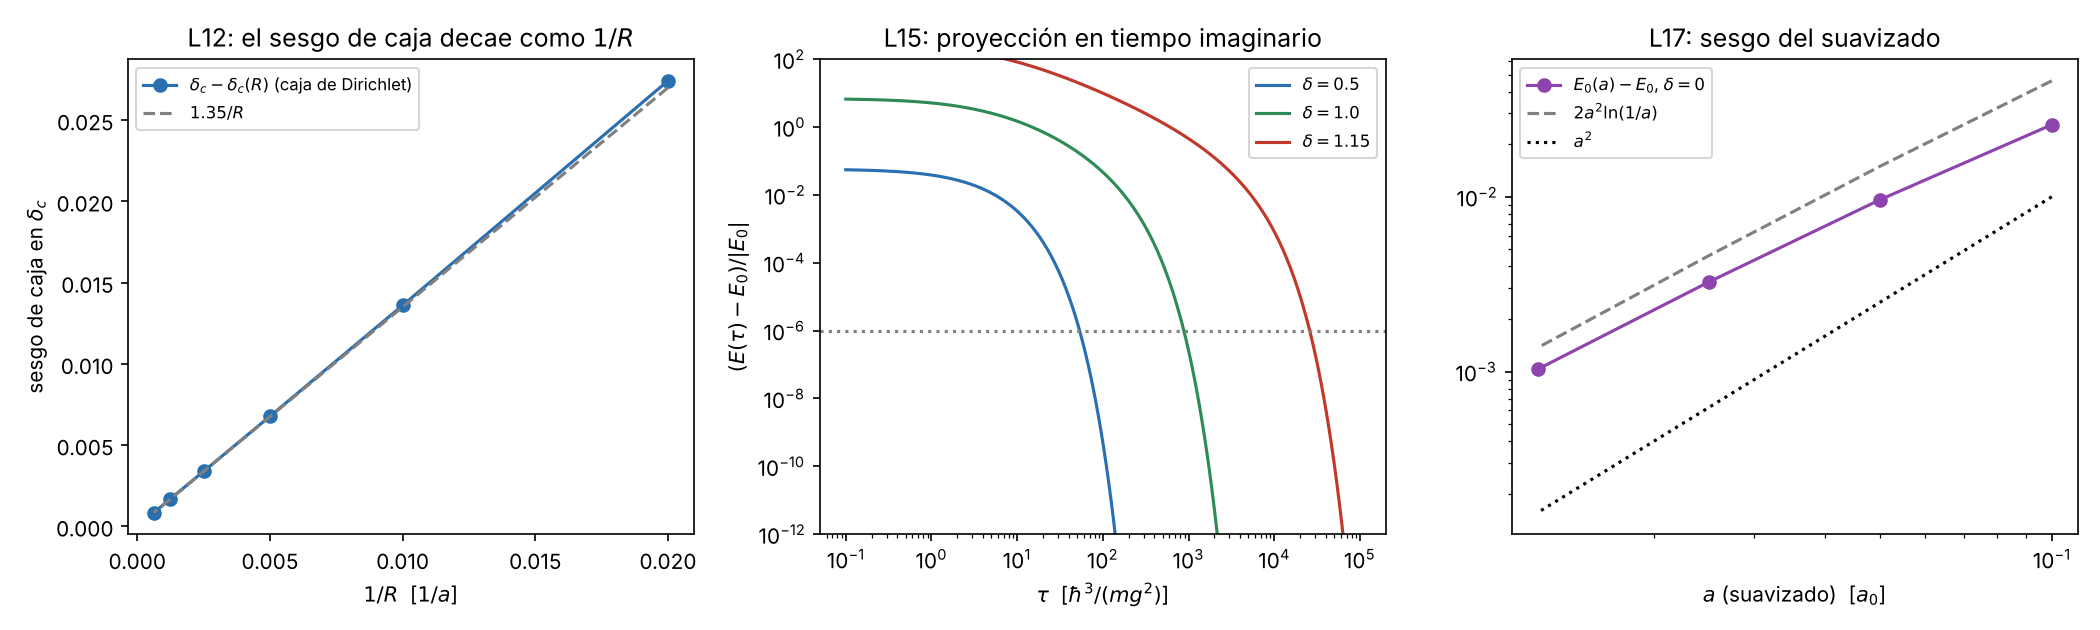
\includegraphics[width=\textwidth]{figuras/07_limites_fisicos.png}
\caption{Izquierda: sesgo de la caja de Dirichlet en el umbral, lineal en $1/R$ con pendiente 1.35. Centro: convergencia de $E(\tau)$ hacia $E_0$ para tres valores de $\delta$; el tiempo necesario crece como $1/|E_0|$. Derecha: sesgo del potencial suavizado en $\delta=0$, comparado con $2a^2\ln(1/a)$ y con $a^2$.}
\end{figure}

\subsection{Lo que la IA dijo mal o de forma imprecisa}

\begin{enumerate}
\item \textbf{L13 (error).} La IA afirmó que, sin estado ligado, $E_0R^2\to\pi^2/2$. Eso solo vale para $R\to\infty$; a tamaños accesibles falta la longitud de dispersión. Con $u=A+Br$ a energía cero, $a_{\rm sc}=-A/B$, y la ley correcta es $E_0(R)\simeq\pi^2/[2(R-a_{\rm sc})^2]$. En $\delta=1.3$ el script da $a_{\rm sc}=-11.58$, que predice $E_0R^2=3.964$ y $4.661$ en $R=100$ y $400$, frente a $4.028$ y $4.672$ medidos; en $\delta=2$, $a_{\rm sc}=-1.10$ y el acuerdo es de tres cifras. La consecuencia práctica importa: cerca del umbral $|a_{\rm sc}|$ diverge, así que ``$E_0R^2\approx\pi^2/2$'' no sirve para declarar ``no ligado'' salvo que $R\gg|a_{\rm sc}|$.
\item \textbf{L10 (imprecisión).} El $c\approx0.75$ que dio la IA es la pendiente secante en $[1.05,1.15]$. El cociente $\kappa/(\dc-\delta)$ baja al acercarse al umbral y extrapola a $c=0.741$.
\item \textbf{L11 (imprecisión).} $\langle r\rangle\simeq1/(2\kappa)$ es una ley asintótica: en $\delta=1$ el producto $2\kappa\langle r\rangle$ vale 1.25, no 1; solo a $0.01$ del umbral el error baja al 1~\%.
\item \textbf{L17 (imprecisión).} El término dominante $2a^2\ln(1/a)$ es correcto, pero el siguiente, $Ca^2$ con $C=-2.154$, es grande: en $a=0.0125$ el cociente $\Delta E/(2a^2\ln(1/a))$ es solo 0.75. Además el suavizado desplaza el umbral de forma apreciable ($\dc(0.1)$ es $0.047$ menor), lo que confirma que un resultado suavizado no se puede identificar con el Yukawa sin extrapolar.
\item \textbf{Lo que la IA no dijo.} En $\delta=1.18$, que \emph{sí} está ligado, una caja $R=20$ da $E_0=+2.95\times10^{-3}$: un falso ``no ligado''. Y el sesgo de caja en el umbral es algebraico ($1.35/R$), no exponencial.
\end{enumerate}
En las fórmulas exactas (L2 a L9, L16) no encontramos errores.

\subsection{Ejemplo: el umbral aparente de una sola caja}
\label{sec:caja}

Para ver el sesgo de caja con números concretos calculamos el umbral aparente de una caja de Dirichlet de radio $R$, es decir, el $\delta$ para el que $E_0=0$ con $u(R)=0$. Lo hicimos sin malla (\texttt{06\_fuentes.py}): integrando $u''=-2e^{-\delta r}u/r$ a energía cero con DOP853 y buscando $u(R)=0$.

\begin{table}[H]
\centering
\small
\begin{tabular}{@{}llll@{}}
\toprule
$R$ & $\dc(R)$ & $\dc(R)-\dc$ & $R\,(\dc-\dc(R))$\\
\midrule
100 & 1.177013 & $-1.36\times10^{-2}$ & 1.360\\
200 & 1.183840 & & 1.355\\
400 & 1.187233 & & 1.352\\
800 & 1.188924 & $-1.69\times10^{-3}$ & 1.351\\
\bottomrule
\end{tabular}
\end{table}

El sesgo decrece como $1/R$ con la pendiente 1.35 de L12. La caja sube la energía y adelanta el umbral. En una primera versión estas cifras las habíamos sacado biseccionando el signo de $E_0$ con diferencias finitas de paso $h=0.02$ ($1.17685$ a $1.18870$); en la verificación del 21 de octubre vimos que mezclaban el sesgo de caja con un error de malla de unos $-2\times10^{-4}$, y las rehicimos así. Los valores de la tabla coinciden a $10^{-8}$ con un disparo en mpmath y con un método espectral de Chebyshev.

\subsection{Tabla consolidada de límites de la Fase 1}

\begin{longtable}{@{}L{2.6cm}L{4.4cm}L{6.4cm}@{}}
\toprule
\textbf{Límite} & \textbf{Qué debe ocurrir} & \textbf{Qué se obtuvo}\\
\midrule
\endhead
$\delta\to0$ & hidrógeno: $E_0=-1/2$, $\langle r\rangle=3/2$ & residuo simbólico 0; numérico $-0.500000000$, $1.50000$\\
$\delta$ pequeño & serie hasta $\delta^4$, residuo $O(\delta^5)$ & cociente 30.5 al duplicar $\delta$ (se espera 32)\\
$\delta\to\dc^-$ & $\kappa$ lineal, $E_0$ cuadrática, $\langle r\rangle$ divergente & $\kappa\simeq0.741(\dc-\delta)$; $2\kappa\langle r\rangle=1.013$ en $\delta=1.18$\\
$\delta\ge2$ & ningún estado ligado & Bargmann, Hulthén y numérico ($E_0(2)>0$, estado de caja)\\
excitados & número finito; el $2s$ se desliga antes & $\dc(2s)=0.310209$ (Hulthén: $1/2$)\\
$r\to0$ & $u\simeq r-r^2$ & Frobenius y ajuste numérico ($-0.9998$)\\
$r\to\infty$ & $u\sim e^{-\kappa r}$ sin factor $r^{1/\kappa}$ & comprobado en $r=10$ y 20\\
$R\to\infty$ & $E_0(R)$ decrece; umbral aparente por debajo de $\dc$ & $\dc-\dc(R)\simeq1.35/R$; falso ``no ligado'' con caja pequeña\\
$\tau\to\infty$ & $E(\tau)$ monótona; tiempo $\propto1/|E_0|$ & $\tau|E_0|\approx9$ para error $10^{-6}$\\
$\epsilon\to0$ & sesgo de Trotter $O(\epsilon^2)$ & pendientes 1.989 (oscilador), 1.99 (pares), 1.98 (transferencia)\\
$a_s\to0$ & $\dc(a_s)\to\dc$ desde abajo & extrapolado $1.19061008$\\
$h\to0$ & error $\propto h^2$ & factor 4 al dividir $h$ entre 2\\
dimensiones & un solo grupo adimensional & $\delta=\mu\hbar^2/(mg)$; cambio de $(\hbar,m,g)$ a $\delta$ fijo: $8\times10^{-13}$\\
\bottomrule
\end{longtable}

%======================================================================
\section{Integral de camino euclídea y análisis del peso}
\label{sec:accion}

Script: \texttt{08\_accion\_euclidea.py}.

\textbf{Objetivo del bloque.} Escribir la integral de camino euclídea discreta para $\hat H=-\tfrac12\nabla^2-e^{-\delta r}/r$, decidir si el peso que habría que muestrear es real, positivo y normalizable, y elegir con evidencia la acción para la Fase 2. \textbf{Régimen:} una partícula sin espín en 3D, $\delta\ge0$, tiempo imaginario $\tau$ en unidades $\hbar^3/(mg^2)$. \textbf{Cierre del bloque:} (i) acción, medida, fronteras y estimadores escritos sin saltos; (ii) veredicto sobre el peso demostrado y comprobado numéricamente; (iii) un toy model donde la proyección recupere $E_0$ y el sesgo de Trotter escale como $\epsilon^2$; (iv) un remedio para el Yukawa probado con sesgo controlado.

Notación: $\mathbf r_k$ posición del eslabón $k$; $\epsilon=\beta/M$; $K_0(\mathbf r,\mathbf r';\epsilon)=(2\pi\epsilon)^{-3/2}e^{-|\mathbf r-\mathbf r'|^2/(2\epsilon)}$ núcleo libre; $\rho(\mathbf r,\mathbf r';\epsilon)=\langle\mathbf r|e^{-\epsilon\hat H}|\mathbf r'\rangle$ núcleo exacto; $U=-\ln(\rho/K_0)$ acción de pares.

\subsection{Deducción}

\textbf{Propagador.} $G(\mathbf r_b,\mathbf r_a;\beta)=\langle\mathbf r_b|e^{-\beta\hat H}|\mathbf r_a\rangle$ cumple $\partial_\beta G=-\hat H_bG$ con $G\to\delta^3(\mathbf r_b-\mathbf r_a)$ cuando $\beta\to0$, y $G=\sum_n\psi_n(\mathbf r_b)\psi_n^*(\mathbf r_a)e^{-\beta E_n}$ (más el continuo).

\textbf{Factorización.} Escribimos $e^{-\beta\hat H}=(e^{-\epsilon\hat H})^M$ e insertamos $M-1$ resoluciones de la identidad:
\[
G(\mathbf r_M,\mathbf r_0;\beta)=\int\prod_{k=1}^{M-1}\dd^3r_k\ \prod_{k=0}^{M-1}\rho(\mathbf r_{k+1},\mathbf r_k;\epsilon).
\]
Hasta aquí todo es exacto.

\textbf{Aproximación primitiva.} Con Trotter simétrico y $\langle\mathbf r|e^{-\epsilon\hat T}|\mathbf r'\rangle=K_0$,
\[
\rho(\mathbf r_{k+1},\mathbf r_k;\epsilon)\approx e^{-\epsilon V(\mathbf r_{k+1})/2}\,K_0(\mathbf r_{k+1},\mathbf r_k;\epsilon)\,e^{-\epsilon V(\mathbf r_k)/2},
\]
con error $O(\epsilon^3)$ por paso si $V$ es suave, es decir $O(\epsilon^2)$ en total.

\textbf{Acción discreta y medida.} Con traza periódica ($\mathbf r_M\equiv\mathbf r_0$),
\[
S_E=\sum_{k=0}^{M-1}\left[\frac{|\mathbf r_{k+1}-\mathbf r_k|^2}{2\epsilon}+\epsilon V(\mathbf r_k)\right],\qquad \text{medida }\prod_k\frac{\dd^3r_k}{(2\pi\epsilon)^{3/2}}.
\]
En el límite continuo $S_E\to\int_0^\beta\dd\tau\,[\tfrac12\dot{\mathbf r}^2+V(\mathbf r)]$, que coincide con la acción euclídea de Kleinert (ec.~2.378) con $m=\hbar=1$. Restaurando constantes, los dos términos son $m|\Delta\mathbf r|^2/(2\hbar\epsilon)$ y $\epsilon V/\hbar$, ambos adimensionales.

\textbf{Fronteras.} Para el propagador, extremos fijos $\mathbf r_0=\mathbf r_a$, $\mathbf r_M=\mathbf r_b$. Para la función de partición $Z(\beta)=\Tr e^{-\beta\hat H}$, caminos cerrados. Ojo: en volumen infinito $\hat H$ tiene espectro continuo $[0,\infty)$ y $Z=\infty$; por eso o se usa una caja de radio $R$ o se proyecta desde una función de prueba.

\textbf{Feynman-Kac.} Para $M\to\infty$, $G=K_0(\mathbf r_b,\mathbf r_a;\beta)\,\mathbb E_{\rm puente}\big[\exp\big(-\int_0^\beta V(\mathbf X_\tau)\dd\tau\big)\big]$ con $\mathbf X_\tau$ un puente browniano. Para el Yukawa esta esperanza es finita, aunque cada aproximación primitiva de tiempo finito no lo sea (lo vemos enseguida).

\textbf{Estimadores de energía.}
\begin{enumerate}
\item Termodinámico, $E=-\partial_\beta\ln Z_M$ a $M$ fijo:
$E_T=\frac{3}{2\epsilon}-\frac{1}{M}\sum_k\frac{|\mathbf r_{k+1}-\mathbf r_k|^2}{2\epsilon^2}+\frac1M\sum_kV(\mathbf r_k)$. Su varianza crece como $1/\epsilon$.
\item Virial, con $\langle\hat T\rangle=\tfrac12\langle\mathbf r\cdot\nabla V\rangle$:
$E_V=\frac1M\sum_k\big[V+\tfrac12rV'\big]_{\mathbf r_k}=-\frac1M\sum_k\frac{e^{-\delta r_k}(1-\delta r_k)}{2r_k}$, que para $\delta=0$ da $-1/2$. Solo vale para $\beta\to\infty$ y estado ligado en volumen infinito.
\item Proyección, con una prueba $\psi_T$ no ortogonal al fundamental:
$E_{\rm eff}(\tau)=-\frac1\epsilon\ln\frac{\langle\psi_T|e^{-(\tau+\epsilon)\hat H}|\psi_T\rangle}{\langle\psi_T|e^{-\tau\hat H}|\psi_T\rangle}=E_0+O\big(e^{-(E_1-E_0)\tau}\big)$.
\end{enumerate}

\textbf{Versión radial $\ell=0$.} Con $\psi=u/(\sqrt{4\pi}r)$ el problema es unidimensional en $r>0$ con $u(0)=0$, y el núcleo libre con Dirichlet es el de imágenes,
\[
K_D(r,r';\epsilon)=\frac{1}{\sqrt{2\pi\epsilon}}\left[e^{-(r-r')^2/2\epsilon}-e^{-(r+r')^2/2\epsilon}\right].
\]
Con sympy comprobamos que promediar $K_0$ 3D sobre el ángulo da exactamente $rr'\int\dd\Omega\,K_0=K_D$: la imagen no es un truco sino la proyección exacta del núcleo libre en la onda $s$. Esta versión solo vale en el sector $\ell=0$ (para $\ell>0$ aparece la barrera centrífuga, otra singularidad) y $K_D>0$, así que no sirve para estados excitados con nodos.

\subsection{¿El peso es real, positivo y normalizable?}
\label{sec:peso}

\textbf{Veredicto.} El peso primitivo $e^{-S_E}$ es \textbf{real y positivo} para todo camino, pero \textbf{no es normalizable}: la integral sobre cualquier coordenada intermedia diverge en $r\to0$, para todo $\epsilon>0$ y todo $\delta\ge0$. El núcleo exacto sí es normalizable. El problema es de la discretización, no de la física.

\textbf{Real y positivo.} $K_0>0$ y $e^{-\epsilon V}=\exp(+\epsilon e^{-\delta r}/r)>0$; en tiempo imaginario, sin campo magnético y con una sola partícula no hay fases. No hay problema de signo.

\textbf{No normalizable: demostración.} Fijemos los vecinos $\mathbf r_{k\pm1}$ y miremos la integral sobre $\mathbf r_k$ cerca del origen. $K_0$ es acotado y en $\mathbf r_k=0$ vale $(2\pi\epsilon)^{-3/2}e^{-r_{k\pm1}^2/2\epsilon}>0$, así que existe $c>0$ tal que
\[
\int_{r<r_1}\dd^3r_k\,K_0K_0\,e^{\epsilon e^{-\delta r_k}/r_k}\ \ge\ c\,4\pi\int_0^{r_1}r^2e^{\epsilon e^{-\delta r_1}/r}\,\dd r=\infty,
\]
porque con $x=1/r$ la integral $\int^\infty x^{-4}e^{\epsilon'x}\dd x$ diverge. El factor $r^2$ de la medida pierde frente a $e^{\epsilon/r}$, y el gaussiano no compensa porque es acotado: su supresión actúa a distancias $\sim\sqrt\epsilon$ del vecino, no en el origen. Basta una coordenada intermedia (dos pasos de tiempo), de acuerdo con Kleinert: ``Feynman's time-sliced formula, however, diverges even for two time slices''.

\textbf{Comprobación numérica.} Con vecinos en $|\mathbf r_{k\pm1}|=1$ e $I(r_{\min})=\int_{r>r_{\min}}\dd^3r\,K_0K_0\,e^{-\epsilon V}$ (mpmath, 30 dígitos), para $\delta=0$:

\begin{table}[H]
\centering
\small
\begin{tabular}{@{}llll@{}}
\toprule
$\epsilon$ & $\log_{10}I(r_{\min}=0.1)$ & $\log_{10}I(r_{\min}=10^{-3})$ & $I$/asíntota en $10^{-3}$\\
\midrule
0.05 & 0.32 & 4.98 & 1.089\\
0.10 & $-0.11$ & 29.81 & 1.042\\
0.20 & $-0.51$ & 74.20 & 1.021\\
\bottomrule
\end{tabular}
\end{table}

La asíntota es $I\simeq4\pi g(0)\,r_{\min}^4e^{\epsilon e^{-\delta r_{\min}}/r_{\min}}/\epsilon$ y el cociente tiende a 1. La divergencia solo se hace visible cuando $\epsilon/r_{\min}$ llega a unas decenas: con $\epsilon=0.1$, $I$ casi no cambia entre $r_{\min}=0.1$ y $0.01$ y luego explota ($\log_{10}I=2.75$, 29.76 y 71.97 para $r_{\min}=3\times10^{-3}$, $10^{-3}$ y $5\times10^{-4}$). Una simulación que solo explore $r\gtrsim0.01$ no lo notaría, y ese es justamente el peligro.

\textbf{El apantallamiento no ayuda.} $V=-1/r+\delta-\delta^2r/2+O(r^2)$, así que $e^{-\epsilon V}=e^{\epsilon/r}e^{-\epsilon\delta}(1+O(r))$: el Yukawa solo cambia la constante. Numéricamente, $I(\dc)/I(0)=0.88782$ en $r_{\min}=10^{-3}$, $\epsilon=0.1$, frente a $e^{-\epsilon\dc}=0.88775$. El apantallamiento actúa a $r\sim1/\delta$, lejos de donde está la divergencia.

\textbf{El núcleo exacto sí es normalizable.} Por la desigualdad de Hardy en 3D, $\|\psi/r\|\le2\|\nabla\psi\|$; para $\|\psi\|=1$ y $k=\|\nabla\psi\|$,
\[
\langle\psi|\hat H_{\delta=0}|\psi\rangle\ge\tfrac12k^2-\|\psi/r\|\ge\tfrac12k^2-2k\ge-2 .
\]
Como $0<e^{-\delta r}/r\le1/r$, también $\hat H_\delta\ge\hat H_0\ge-2$ (el valor exacto es $-1/2$). Con $\hat H$ acotado inferiormente, $e^{-\epsilon\hat H}$ es acotado y positivo, $\rho$ es finito y $\int\dd^3r'\,\rho(\mathbf r,\mathbf r';\epsilon)\rho(\mathbf r',\mathbf r'';\epsilon)=\rho(\mathbf r,\mathbf r'';2\epsilon)<\infty$. Esto prueba H8.

Para verlo numéricamente calculamos $\rho_{\ell=0}(r,r;\epsilon=0.1)$ por descomposición espectral del hamiltoniano radial discretizado (caja $R=4$, $h=0.005$ y $0.0025$, que coinciden en $10^{-4}$) y la acción de pares $U=-\ln(\rho/K_D)$:

\begin{table}[H]
\centering
\small
\begin{tabular}{@{}lllll@{}}
\toprule
$r$ & $U(\delta=0)$ & $\epsilon V(\delta=0)$ & $U(\dc)$ & $\epsilon V(\dc)$\\
\midrule
0.02 & $-0.769$ & $-5.000$ & $-0.662$ & $-4.882$\\
0.10 & $-0.630$ & $-1.000$ & $-0.524$ & $-0.888$\\
0.50 & $-0.218$ & $-0.200$ & $-0.128$ & $-0.110$\\
1.50 & $-0.067$ & $-0.067$ & $-0.012$ & $-0.011$\\
\bottomrule
\end{tabular}
\end{table}

$U$ es finita en $r\to0$ y se pega a $\epsilon V$ para $r\gg\sqrt\epsilon$; además $\rho(r,r)/r^2\approx55$ en $r=0.01$ y $0.02$, es decir $\rho\sim r^2$, como pide $u(0)=0$.

\begin{figure}[H]
\centering
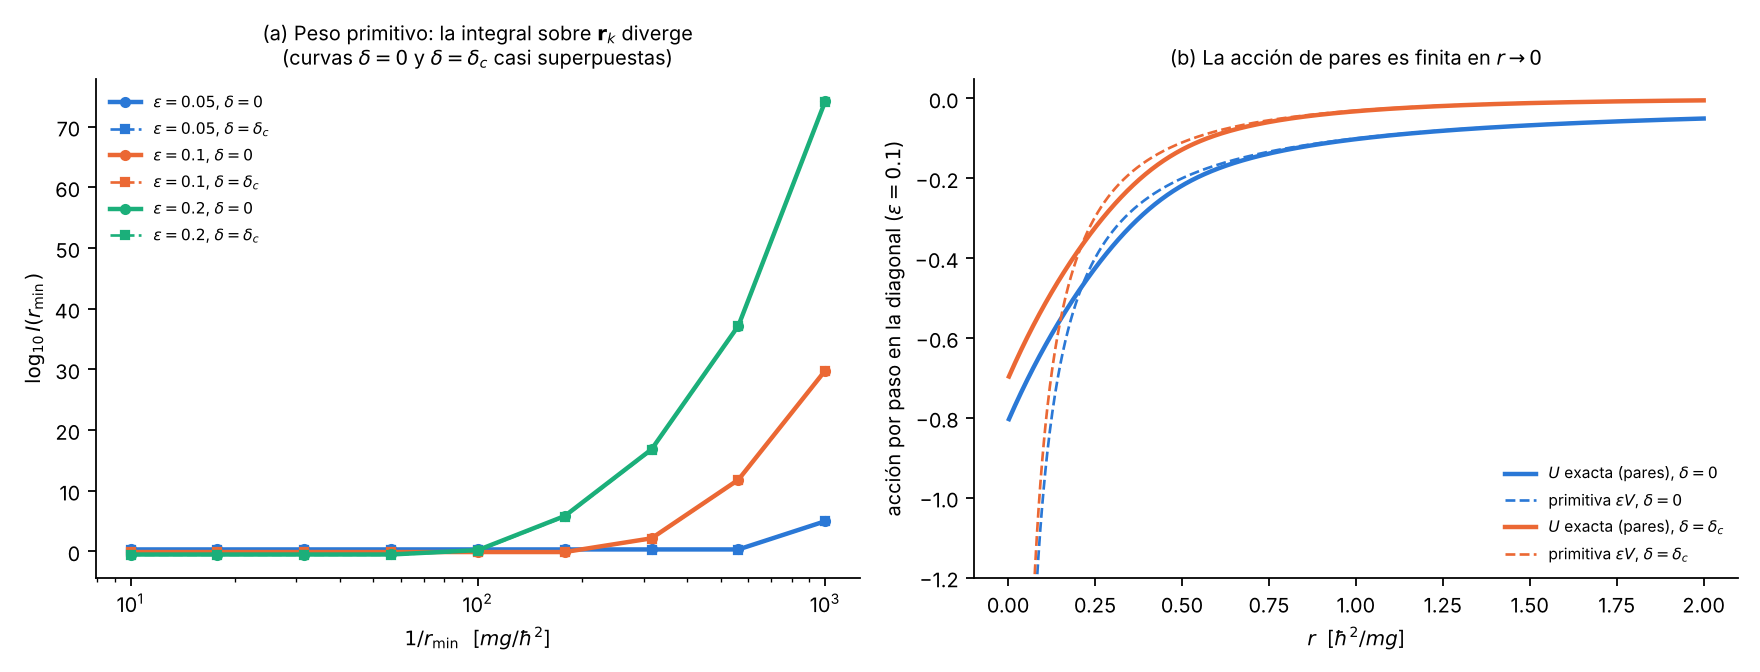
\includegraphics[width=\textwidth]{figuras/08_divergencia_peso.png}
\caption{(a) $\log_{10}I(r_{\min})$ frente a $1/r_{\min}$ para tres $\epsilon$ y $\delta\in\{0,\dc\}$; las curvas casi se superponen porque el apantallamiento no cambia nada. (b) Acción por paso en la diagonal: la exacta (pares) es finita en el origen; la primitiva $\epsilon V$ se va a $-\infty$.}
\end{figure}

\textbf{¿Por qué falla la primitiva?} Supone que $V$ es casi constante en una región de tamaño $\sqrt\epsilon$ alrededor de cada eslabón, y cerca de $r=0$ eso es falso. El núcleo exacto ``sabe'' que confinar la partícula en $r\lesssim\sqrt\epsilon$ cuesta energía cinética (principio de incertidumbre) y por eso $U$ satura; la primitiva separa cinética y potencial y premia sin límite el colapso de un eslabón sobre el centro. Es el análogo discreto del colapso clásico en $-1/r$.

\subsection{Remedios y cuál elegimos}

\begin{longtable}{@{}L{3.4cm}L{2.6cm}L{4.0cm}L{3.8cm}@{}}
\toprule
\textbf{Remedio} & \textbf{Peso} & \textbf{Qué cuesta} & \textbf{Evidencia}\\
\midrule
\endhead
R1. Acción de pares: núcleo exacto de Coulomb $\rho_C$ más el resto $W=(1-e^{-\delta r})/r$ & real, $>0$, normalizable & tabular $\rho_C(r,r';\epsilon)$ & $0\le W\le\delta$; sesgo $O(\epsilon^2)$ comprobado\\
R2. Kustaanheimo-Stiefel / Duru-Kleinert & positivo tras la transformación & reparametrizar el tiempo, espacio 4D con una ligadura & solo bibliográfica\\
R3. Suavizado $V_{a_s}=-e^{-\delta r}/\sqrt{r^2+a_s^2}$ & normalizable & sesgo $\sim a_s^2\ln(1/a_s)$; exige extrapolar $a_s\to0$ & tabla de abajo\\
R4. Orden superior (Takahashi-Imada) & $W_{TI}=V+\tfrac{\epsilon^2}{24}|\nabla V|^2$ normalizable & regulariza ``por accidente'' donde la expansión ya no vale & $\log_{10}I=-0.135083$ estable hasta $r_{\min}=10^{-5}$\\
R5. Radial con imagen & positivo, pero con $e^{-\epsilon V}$ primitivo \emph{sigue divergiendo} & es un marco, no un remedio & $\log_{10}I$: $-0.03$, $-0.03$, 3.85, 30.86, 73.07\\
\bottomrule
\end{longtable}

\textbf{Sobre R2.} Fujikawa resume que Duru y Kleinert resolvieron exactamente la función de Green del hidrógeno con un tiempo reescalado y la transformación de Kustaanheimo y Stiefel; Kleinert dice que estas transformaciones llevan el problema ``back to a Feynman type formula with a bounded potential in an auxiliary space''. Una observación nuestra, sin desarrollar: en las variables KS $r=|\mathbf u|^2$ y $rV(r)=-e^{-\delta|\mathbf u|^2}$, que es acotado y suave. Faltaría derivar factores, ligadura y correcciones de corte temporal.

\textbf{Sobre R3.} Resultados del disparo con el potencial suavizado:

\begin{table}[H]
\centering
\small
\begin{tabular}{@{}lll@{}}
\toprule
$a_s$ & $\dc(a_s)-\dc$ & $E_0(a_s)+\tfrac12$ ($\delta=0$)\\
\midrule
0.1 & $-4.7\times10^{-2}$ & $2.6\times10^{-2}$\\
0.025 & $-6.4\times10^{-3}$ & $3.3\times10^{-3}$\\
0.00625 & $-6.4\times10^{-4}$ & $3.1\times10^{-4}$\\
0.003125 & $-1.9\times10^{-4}$ & $9.2\times10^{-5}$\\
\bottomrule
\end{tabular}
\end{table}

A primer orden $\Delta E=\int|\psi|^2(V_{a_s}-V)\dd^3r$ y $1/r-1/\sqrt{r^2+a_s^2}\sim a_s^2/2r^3$ dan una integral logarítmica, $\Delta E\approx2a_s^2\ln(1/a_s)$ para el hidrógeno. El cociente medido sube de 0.71 a 0.81 en los cuatro menores $a_s$. El ajuste $f_0+c_1a_s^2\ln a_s+c_2a_s^2$ da $E_0\to-0.49999988$ ($c_1=-1.998$, cerca del $-2$ predicho) y $\dc\to1.19061008$ ($-2.3\times10^{-6}$ de la literatura), mientras que el menor $a_s$ sin extrapolar se equivoca en $-1.9\times10^{-4}$. Conclusión: \textbf{$a_s$ tiene que declararse y el resultado no se puede identificar con el Yukawa sin extrapolar $a_s\to0$}.

\begin{figure}[H]
\centering
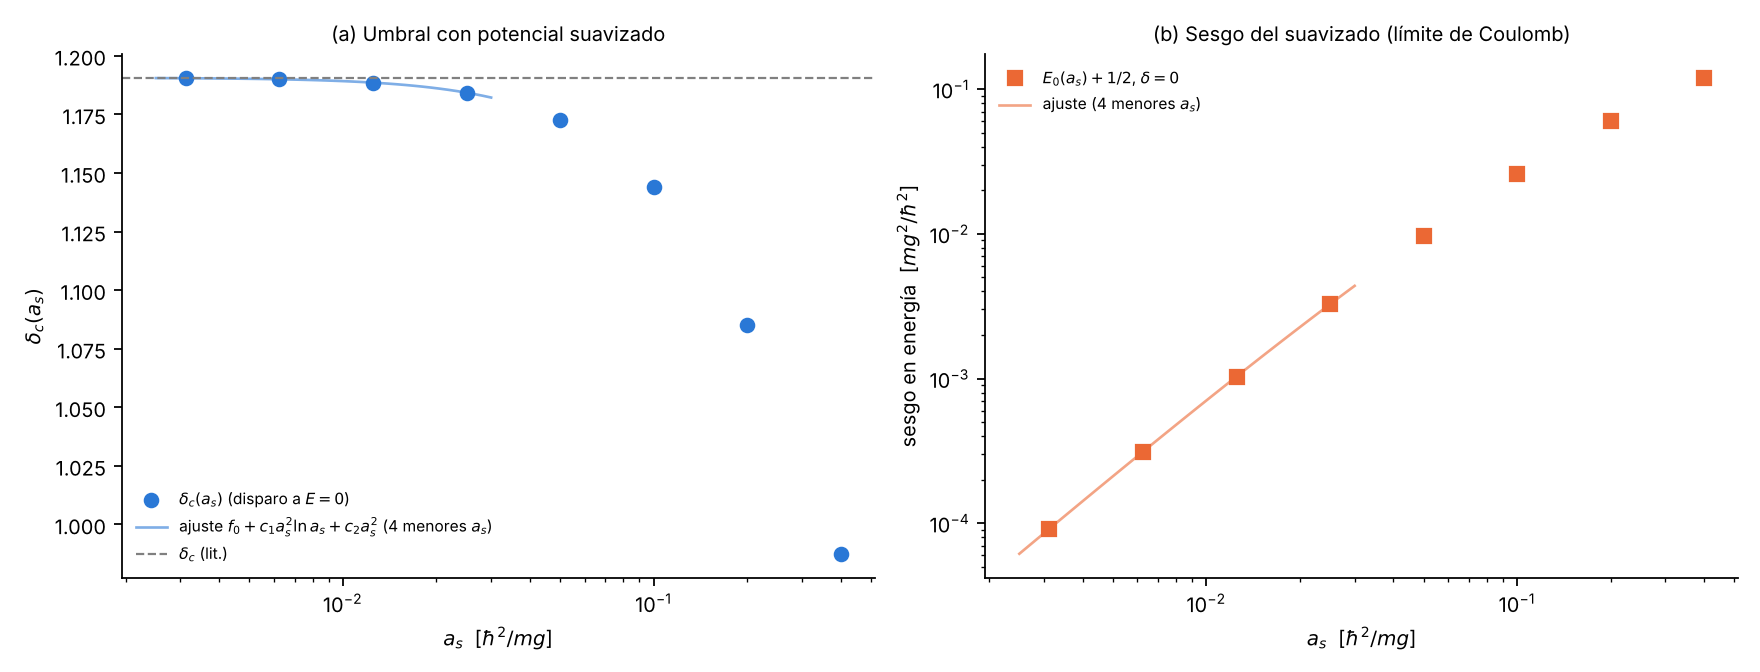
\includegraphics[width=\textwidth]{figuras/08_suavizado.png}
\caption{(a) $\dc(a_s)$ y su extrapolación; (b) sesgo de energía en el límite de Coulomb con el ajuste en la región de $a_s$ pequeño.}
\end{figure}

\textbf{Elección para la Fase 2: R1 en la formulación radial (R5 como marco).} (1) El peso es real, positivo y normalizable sin parámetro artificial. (2) La singularidad entera se trata exactamente con un objeto que no depende de $\delta$ (el núcleo de Coulomb, un problema resuelto e independiente del Yukawa, así que no hay circularidad). (3) El resto $W$ es acotado y suave, de modo que la factorización simétrica tiene su sesgo ordinario $O(\epsilon^2)$. (4) En $\delta=0$ el método es exacto para todo $\epsilon$, lo que da un control gratis. R3 queda como control cruzado, siempre con extrapolación.

\subsection{Toy model de la integral de camino: oscilador armónico 1D}
\label{sec:oscilador}

Lo elegimos porque todo es gaussiano y hay solución discreta exacta: $V=x^2/2$, $E_0=1/2$. Con la prueba $e^{-\alpha x^2/2}$ en la matriz de transferencia simétrica $T=e^{-\epsilon W/2}K_0e^{-\epsilon W/2}$ se resuelven $\alpha(\epsilon)$ y el autovalor:
\[
E_0^{\rm prim}(\epsilon)=\frac12-\frac{\epsilon^2}{48}+\frac{3\epsilon^4}{1280}+\dots,\qquad E_0^{\rm TI}(\epsilon)=\frac12-\frac{\epsilon^4}{1440}+\dots
\]
El estimador termodinámico a $\beta\to\infty$ tiende a $\tfrac12-\epsilon^2/16$, con otro coeficiente: a $\epsilon$ finito los dos no se deben comparar entre sí sin extrapolar.

\begin{itemize}
\item \textbf{Matriz de transferencia numérica} (malla $x\in[-9,9]$, $\dd x\le\sqrt\epsilon/12$): los autovalores coinciden con la fórmula analítica en las 10 cifras impresas para 7 valores de $\epsilon\in[0.125,1]$. Pendiente log-log del sesgo: \textbf{1.989} (primitiva, se espera 2) y \textbf{3.985} (TI, se espera 4); coeficientes en $\epsilon=0.125$: $-0.02080$ frente a $-1/48=-0.02083$ y $-6.93\times10^{-4}$ frente a $-1/1440$.
\item \textbf{Proyección} con $\psi_T=e^{-|x|}$, $\epsilon=0.1$: $E_{\rm eff}-E_0(\epsilon)=1.05\times10^{-2}$, $6.4\times10^{-5}$, $7.7\times10^{-7}$, $3.1\times10^{-10}$ en $\tau=0.5$, 2, 4, 7.9. La tasa medida es 2.0011 y la brecha discreta $E_2-E_0=1.9992$: la prueba par no tiene componente en $E_1$, así que la tasa es $2\omega$.
\item \textbf{Dos derivadas de $\ln Z$.} A $\epsilon$ fijo variando $M$ se obtiene la energía del autovalor (1.0853, 0.5523, 0.5023, 0.4998 para $\beta=1,3,6,10$, que tiende a 0.49979); a $M$ fijo variando $\epsilon$ se obtiene el estimador termodinámico, $E_{\rm termo}=\tfrac12\theta'(\epsilon)\coth(M\theta/2)$ con $\cosh\theta=1+\epsilon^2/2$ (1.0810, 0.5518, 0.5019, 0.4994, que tiende a $\tfrac12-\epsilon^2/16=0.499375$). Cada estimador a $\epsilon$ finito se compara con su propio valor discreto.
\item \textbf{PIMC primitivo} (Metropolis con actualización par/impar y movimiento rígido, $\beta=10$, $M=40$, $\epsilon=0.25$, $2\times10^5$ barridos): $E_T=0.4957\pm0.0022$ (exacto discreto 0.4961) y $E_V=0.4950\pm0.0030$ (exacto discreto 0.4962), a $0.2\sigma$ y $0.4\sigma$.
\end{itemize}

\begin{figure}[H]
\centering
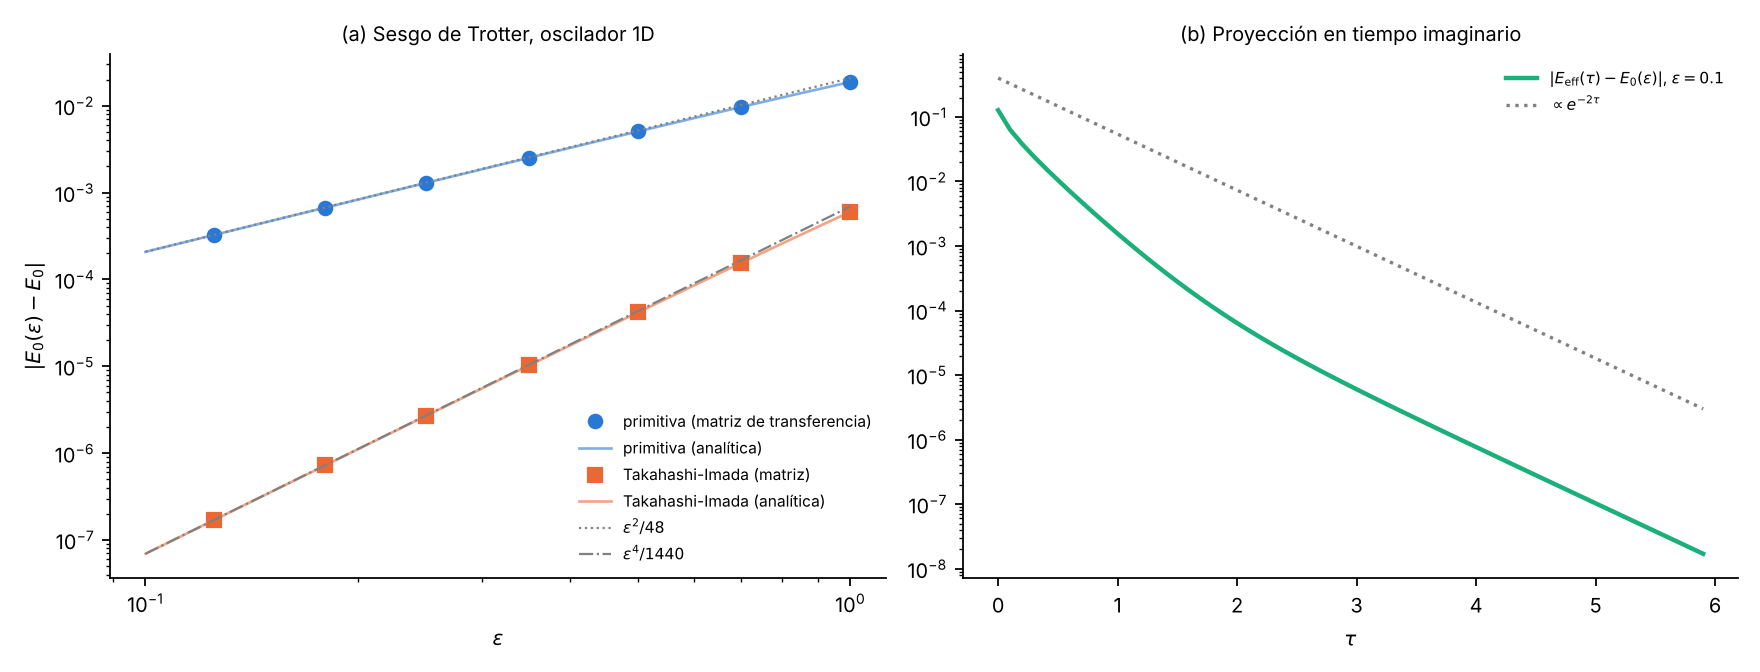
\includegraphics[width=\textwidth]{figuras/08_toy_trotter.png}
\caption{(a) Sesgo $|E_0(\epsilon)-E_0|$ en el oscilador: primitiva $\propto\epsilon^2$, Takahashi-Imada $\propto\epsilon^4$; puntos numéricos sobre las curvas analíticas. (b) Convergencia de la proyección $\propto e^{-2\tau}$.}
\end{figure}

\subsection{Prueba de concepto de la acción elegida}

Matriz de transferencia radial $T=e^{-\epsilon W/2}\rho_C(\epsilon)e^{-\epsilon W/2}$, con $\rho_C$ espectral del Coulomb puro y $W=(1-e^{-\delta r})/r$, comparada con el autovalor exacto \emph{en la misma malla} para aislar el sesgo de Trotter del error de malla:

\begin{table}[H]
\centering
\small
\begin{tabular}{@{}lll@{}}
\toprule
$\epsilon$ & $E_0(\epsilon)$, $\delta=0.5$ & $E_0(\epsilon)$, $\delta=1.0$\\
\midrule
0.8 & $-0.14822503$ & $-0.01074614$\\
0.2 & $-0.14808597$ & $-0.01027349$\\
0.05 & $-0.14807677$ & $-0.01024207$\\
malla, exacto & $-0.14807615$ & $-0.01023994$\\
\bottomrule
\end{tabular}
\end{table}

La pendiente del sesgo es \textbf{1.99} en los dos casos. El peso nunca diverge y el sesgo es $O(\epsilon^2)$ con coeficiente pequeño ($2.5\times10^{-6}$ y $8.5\times10^{-6}$ en $\epsilon=0.1$), aunque relativamente crece hacia el umbral ($8\times10^{-4}$ de $|E_0|$ en $\delta=1$). La diferencia entre ``malla, exacto'' y los valores de la sección~\ref{sec:numerico} ($-0.14811702$ y $-0.01028579$) es error de la malla gruesa usada aquí ($h=0.02$ y $0.035$), no de Trotter.

\begin{figure}[H]
\centering
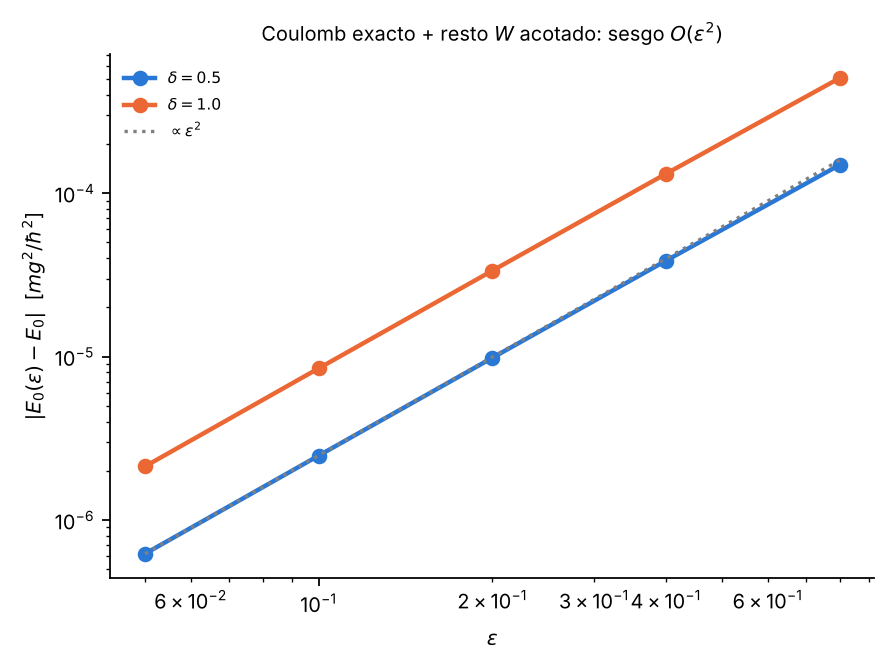
\includegraphics[width=0.6\textwidth]{figuras/08_pares_coulomb.png}
\caption{Sesgo de la acción de pares de Coulomb más el resto $W$, para dos valores de $\delta$.}
\end{figure}

\subsection{Problemas detectados en las fuentes}

\begin{itemize}
\item \textbf{Supuesto implícito.} Saporiti (2020) escribe que la densidad $\omega=e^{-S_E}/\int e^{-S_E}$ tiene integral 1: presupone la normalizabilidad que aquí falla. Kleinert sí lo advierte para Coulomb.
\item \textbf{Posible error de transcripción.} En la transcripción de Kleinert (ec.~2.376) la medida aparece como $\dd x_n/\sqrt{2\pi\beta/M}$; por la integral gaussiana debería ser $\sqrt{2\pi\hbar\epsilon/M}$. Queda por cotejar con el PDF.
\item \textbf{Posible error en una fuente.} Saporiti (ec.~24) escribe el estimador cinético con signo $+$ y sin la constante $1/(2\delta\tau)$; así su promedio diverge como $1/\delta\tau$, no solo su varianza. El estimador correcto (arriba) lleva signo $-$ y la constante. No pudimos decidir si es error del original o de la transcripción.
\item \textbf{Anomalía.} Que la integral con Takahashi-Imada converja no prueba que TI sea de orden 4 para $1/r$: el término correctivo domina justo donde la expansión en conmutadores no converge.
\end{itemize}

%======================================================================
\section{Plan de cómputo para las Fases 2 a 4}
\label{sec:plan}

Script de prueba: \texttt{09\_prueba\_costos.py}. El objetivo de este bloque es convertir lo anterior en un plan ejecutable que llegue a lo que pide la guía para el proyecto 05: ``un intervalo defendible para $\mu_c$ y gráficas de energía y radio característico'', con ``comparación de varias cajas y cota documentada para el umbral''. Consideramos el plan completo si cada observable tiene un método de tiempo imaginario y una referencia independiente, parámetros concretos, un criterio de aceptación cuantitativo, al menos dos fuentes de error con su forma de estimarlas y un costo medido, no supuesto.

\subsection{Observables}

\begin{table}[H]
\centering
\small
\begin{tabular}{@{}lL{5.3cm}L{6.2cm}@{}}
\toprule
\textbf{Símbolo} & \textbf{Definición} & \textbf{Para qué sirve}\\
\midrule
$E_0(\delta)$ & menor autovalor; en tiempo imaginario, límite de proyección o autovalor de la transferencia & observable principal; su signo \emph{no} basta para decidir enlace\\
$\langle r\rangle$ & $\int r\,u^2\dd r/\int u^2\dd r$ & radio característico; diverge como $(\dc-\delta)^{-1}$\\
$\langle r^2\rangle^{1/2}$ & raíz del segundo momento & más sensible a la cola\\
$\langle r\rangle/R$ & radio relativo a la caja & ligado: $\to0$ al crecer $R$; estado de caja: $\to1/2$\\
$F_{1/2}(R)$ & $\int_0^{R/2}u^2\dd r\big/\int_0^Ru^2\dd r$ & ligado: $\to1$; estado de caja: $\to1/2$\\
$\kappa$ & $\sqrt{-2E_0}$ & ley lineal $\kappa\simeq0.741(\dc-\delta)$ para extrapolar\\
\bottomrule
\end{tabular}
\end{table}

En tiempo imaginario, $E_0$ se mide con el estimador mixto en los extremos del camino y $\langle r\rangle$, $\langle r^2\rangle$ con el eslabón central, que muestrea $|e^{-\tau\hat H/2}u_T|^2$ y es un estimador puro. No presentaremos un promedio mixto de $r$ como si fuera puro.

\textbf{Referencia independiente.} El solucionador radial de la sección~\ref{sec:numerico}, que cuesta de 0.004 a 0.05~s por punto y se corre en cada punto donde se corra la integral de camino. Por ejemplo, en $\delta=0.2$ ($R=60$) da $E_0=-0.32680851$, $\langle r\rangle=1.5497$, $\langle r^2\rangle^{1/2}=1.7961$, y en $\delta=1.1$ ($R=370$) $E_0=-0.00228724$, $\langle r\rangle=8.2776$. \textbf{Cuidado con la circularidad:} la tabla de la acción de pares se calcula con la misma discretización que el solucionador radial, aunque solo para $\delta=0$. Para que la comparación no sea circular, la tabla no contiene $\delta$, se extrapola en su paso de malla y la integral de camino usa otra discretización (Nyström o Monte Carlo en $r$ continuo).

\subsection{Formulación elegida}

Sector $\ell=0$, $u(0)=0$, $\epsilon=\tau/M$, acción por eslabón
\[
T(r,r';\epsilon)=K_D(r,r';\epsilon)\,e^{-U_C(r,r';\epsilon)}\,e^{-\epsilon[W(r)+W(r')]/2},\qquad W(r)=\frac{1-e^{-\delta r}}{r}\in[0,\delta],
\]
con $U_C=-\ln(\rho_C/K_D)$ la acción de pares exacta del Coulomb puro. \textbf{Peso:} real, positivo y normalizable ($U_C(0.02,0.02;0.1)=-0.7689$, finita). La acción primitiva con $1/r$ desnudo queda prohibida.

$U_C$ se tabula espectralmente en una caja $R_{\rm tab}=14$ para $r,r'\le10$ y $|r-r'|\le\max(2,7\sqrt\epsilon)$; fuera se usa $U_C\approx\tfrac\epsilon2[V_C(r)+V_C(r')]$, que en $r=r'=9$ coincide con la tabla en cinco cifras. Con $h_{\rm tab}=0.01$ y $0.005$ el Coulomb de la red da $-0.4999875$ y $-0.4999969$; la diferencia máxima entre tablas es $5.3\times10^{-5}$ y se elimina con Richardson.

La misma integral de camino se evalúa de dos formas: (1) \textbf{determinista}, como matriz de transferencia en banda (Nyström con la regla del trapecio, $h=0.02$), cuyo mayor autovalor da $E_0(\epsilon)$ en el límite $\tau\to\infty$; y (2) \textbf{estocástica}, con PIGS (caminos abiertos con peso $u_T(r_0)\prod_kT\,u_T(r_M)$, $u_T=re^{-r}$), que cumple la cúspide pero tiene la cola equivocada para $\delta>0$, como debe ser una prueba no exacta. Movimientos: rebrote de segmentos de 10 eslabones por puente browniano, rebrote de extremos y un cambio global de escala $r\to\lambda r$. No usamos $Z(\beta)$, porque en volumen infinito la traza diverge por el continuo.

\subsection{Parámetros}

\begin{table}[H]
\centering
\small
\begin{tabular}{@{}L{2.4cm}L{3.8cm}L{3.8cm}L{3.8cm}@{}}
\toprule
\textbf{Parámetro} & \textbf{Fase 2} & \textbf{Fase 3} & \textbf{Fase 4}\\
\midrule
Puntos de $\delta$ & 0 (control) y \textbf{0.2} (fuertemente ligado: $E_0=-0.32680851$, $\langle r\rangle=1.5497$) & 0.4, 0.6, 0.8, 1.0, 1.1 & 1.15 a 1.25 alrededor de $\dc$ y bisección\\
Caja $R$ & 40 & $\max(60,25/\kappa)$ y $\{50,\dots,800\}$ para $\delta\ge0.8$ & $\{50,100,200,400,800\}$; hasta 1600 en el radial\\
Paso $\epsilon$ & 0.1 (y 0.2, 0.05) & $\{0.2,0.1,0.05\}$, extrapolación $\epsilon^2$ & igual\\
$\tau$ (PIGS) & 10 ($\delta=0$), 20 ($\delta=0.2$) & $\ge\max(20,9/|E_0|)$; PIGS solo hasta $\delta=1.0$ & la transferencia da $\tau\to\infty$\\
Malla $h$ & 0.02; control 0.04 & 0.02 y 0.01 (Richardson) & igual\\
Cadenas PIGS & 8 de $5\times10^4$ barridos & 8 por punto & solo si hay tiempo\\
Semillas & 20261012 a 20261020; producción 20262000$+k$ & 20263000$+k$ & 20264000$+k$\\
\bottomrule
\end{tabular}
\end{table}

Cerca del umbral, la ley de la sección~\ref{sec:limites} da para $\delta=1.185$ y $1.19$ $\kappa\approx0.0042$ y $0.00045$, y $\langle r\rangle\approx120$ y $1100$: en $\delta=1.19$ ni la caja de 1600 basta y el veredicto puede quedar ``indeterminado'', lo que reportaremos así. $\delta=1.195$ ya está del lado no ligado; ahí lo que crece es la longitud de dispersión ($a_{\rm sc}=-307$; $-143$ en $1.20$ y $-22$ en $1.25$).

\subsection{Prueba de concepto ejecutada}

\textbf{Transferencia en banda} ($\epsilon=0.1$, $h=0.02$, tablas con Richardson):

\begin{table}[H]
\centering
\small
\begin{tabular}{@{}lllllll@{}}
\toprule
$\delta$ & $R$ & $N$ & $E$ (Richardson) & Radial & Diferencia & $\langle r\rangle$\\
\midrule
0.0 & 40 & 2000 & $-0.49999989$ & $-0.5$ & $+1.1\times10^{-7}$ & 1.50000\\
0.2 & 40 & 2000 & $-0.32680852$ & $-0.32680851$ & $-1.5\times10^{-8}$ & 1.54974\\
1.0 & 174 & 8700 & $-0.01029431$ & $-0.01028578$ & $-8.5\times10^{-6}$ & 4.36537\\
1.1 & 370 & 18500 & $-0.00229304$ & $-0.00228724$ & $-5.8\times10^{-6}$ & 8.26847\\
\bottomrule
\end{tabular}
\end{table}

Sin Richardson en la tabla, $\delta=0$ da un error de $2.9\times10^{-5}$ ($h_{\rm tab}=0.01$) y $7.3\times10^{-6}$ ($0.005$): baja como $h_{\rm tab}^2$. En $\delta=1.0$ lo que queda es sesgo de Trotter: con $\epsilon=0.2$, 0.1, 0.05, $E=-0.01031956$, $-0.01029431$, $-0.01028789$, orden aparente \textbf{1.98}, y la extrapolación $\epsilon\to0$ da $-0.01028575$, \textbf{a $3.4\times10^{-8}$ del solucionador radial}.

\textbf{Duración de la proyección} ($\delta=0.2$, $u_T=re^{-r}$): el estimador mixto menos su propio límite vale $+2.3\times10^{-4}$ en $\tau=1$ y baja de forma monótona hasta $+1.0\times10^{-8}$ en $\tau=30$; entre $\tau=20$ y 30 cambia $2.5\times10^{-7}$, así que $\tau=20$ basta. El límite del mixto queda $4.9\times10^{-5}$ por debajo del autovalor de la transferencia en esta red; esa diferencia no cambia con $\epsilon$ y baja un factor 4 al dividir $h$ entre 2, así que es error de malla del núcleo de Coulomb, no de Trotter. Regla adoptada: el mixto y el autovalor solo se comparan tras eliminar el error de malla y el de $\epsilon$.

\textbf{PIGS} (9 cadenas, 1.3 a 3.25~ms por barrido según la carga). Control en $\delta=0$ con $u_T$ exacta: $E_L=-0.5$ con varianza nula; $\langle r\rangle=1.4600\pm0.0380$ y $\langle r^2\rangle=2.830\pm0.173$ frente a 1.5 y 3 ($-1.1\sigma$, $-1.0\sigma$). En $\delta=0.2$ ($\tau=20$, 8 semillas): $E=-0.32687$, $\langle r\rangle=1.539$, $\langle r^2\rangle=3.169$ frente a $-0.32680851$, 1.5497 y 3.2259 del radial: $-0.3\sigma$, $-0.4\sigma$, $-0.4\sigma$. El error entre semillas ($2.1\times10^{-4}$ en $E$) resultó mayor que el de bloques ($1.3\times10^{-4}$): los bloques subestiman la varianza en un factor $2.69$. Regla adoptada: siempre al menos 8 cadenas y se reporta el mayor de los dos errores.

\subsection{Criterio para declarar ``ligado''}
\label{sec:criterio}

La guía exige comparar varias cajas y un observable de localización. Un barrido corto con el solucionador radial ($h=1/40$ y $1/80$, Richardson en $h$) muestra por qué:

\begin{table}[H]
\centering
\small
\begin{tabular}{@{}lllllll@{}}
\toprule
$\delta$ & & $R=50$ & 100 & 200 & 400 & 800\\
\midrule
1.15 (ligado) & $E_0$ & $-3.31\times10^{-4}$ & $-4.51\times10^{-4}$ & $-4.56\times10^{-4}$ & $-4.56\times10^{-4}$ & $-4.56\times10^{-4}$\\
 & $\langle r\rangle/R$; $F_{1/2}$ & 0.239; 0.895 & 0.164; 0.962 & 0.087; 0.998 & 0.044; 1.000 & 0.022; 1.000\\
1.18 (ligado) & $E_0$ & $+3.38\times10^{-4}$ & $+3.21\times10^{-5}$ & $-2.41\times10^{-5}$ & $-3.08\times10^{-5}$ & $-3.10\times10^{-5}$\\
 & $\langle r\rangle/R$; $F_{1/2}$ & 0.293; 0.832 & 0.268; 0.859 & 0.225; 0.904 & 0.153; 0.967 & 0.081; 0.998\\
1.20 (no ligado) & $E_0$ & $+6.44\times10^{-4}$ & $+1.87\times10^{-4}$ & $+5.80\times10^{-5}$ & $+1.84\times10^{-5}$ & $+5.67\times10^{-6}$\\
 & $\langle r\rangle/R$; $F_{1/2}$ & 0.324; 0.790 & 0.331; 0.776 & 0.352; 0.746 & 0.386; 0.695 & 0.426; 0.633\\
1.25 (no ligado) & $\langle r\rangle/R$; $F_{1/2}$ & 0.381; 0.706 & 0.416; 0.650 & 0.450; 0.592 & 0.473; 0.551 & 0.486; 0.527\\
\bottomrule
\end{tabular}
\end{table}

En $\delta=1.18$, que está ligado, las cajas de 50 y 100 dan $E_0>0$: con el signo como único criterio diríamos ``no ligado''. Lo que sí separa los casos es la \emph{tendencia con $R$}: en los ligados $\langle r\rangle/R$ baja y $F_{1/2}$ sube hacia 1; en los no ligados $\langle r\rangle/R$ sube hacia $1/2$ y $F_{1/2}$ baja hacia $1/2$, y eso se ve desde $R=50$. Los valores saturados coinciden con la ley $\kappa=0.7421(\dc-\delta)$: $-4.54\times10^{-4}$ en $\delta=1.15$ y $-3.10\times10^{-5}$ en $1.18$.

También hay que vigilar la malla: en $R=800$, $\delta=1.18$ da $E_0=-2.553\times10^{-5}$ con $h=1/20$, $-2.957\times10^{-5}$ con $1/40$ y $-3.063\times10^{-5}$ con $1/80$, frente a $-3.10\times10^{-5}$ con Richardson (sesgo del 18~\% con $h=1/20$). Un $E_0$ que satura con $R$ no está por eso convergido en $h$.

\textbf{Criterio adoptado} (al menos tres cajas $R_1<R_2<R_3$ con razón 2):
\begin{itemize}
\item \textbf{Ligado} si (a) $E_0(R_2)<0$, $E_0(R_3)<0$ y $|E_0(R_3)-E_0(R_2)|<0.1|E_0(R_3)|$; (a$'$) en cada caja $|E_0(h)-E_0(h/2)|<0.1|E_0|$ y se usa el valor con Richardson; (b) $\langle r\rangle/R$ decrece y $F_{1/2}$ crece en las tres cajas, con $F_{1/2}(R_3)>0.95$; (c) la transferencia da el mismo signo y la misma tendencia.
\item \textbf{No ligado} si $E_0(R)>0$ en todas, $\langle r\rangle/R$ crece y $F_{1/2}$ decrece, y $E_0(R)$ sigue la ley $\pi^2/[2(R-a_{\rm sc})^2]$.
\item \textbf{Indeterminado} en otro caso: se agranda $R$ hasta 1600 (radial) u 800 (transferencia); si sigue así, se reporta como tal y no entra en el intervalo.
\end{itemize}
Con la tabla de arriba, $\delta=1.15$ ya pasa con $R=50$, 100, 200; $\delta=1.18$ solo con $R=200$, 400, 800; y $\delta=1.20$ cumple las dos tendencias de ``no ligado'' desde $R=50$. El intervalo de la Fase 4 será el par más cercano de puntos decididos, refinado por bisección hasta un ancho $\le0.005$, y se contrastará con dos estimaciones que no usan el signo: la extrapolación de $\kappa\to0$ y el umbral de caja corregido con $1.35/R$.

\subsection{Controles y criterios de aceptación}
\label{sec:controles}

\begin{longtable}{@{}L{4.2cm}L{5.6cm}L{3.6cm}@{}}
\toprule
\textbf{Control} & \textbf{Criterio} & \textbf{Estado en la prueba}\\
\midrule
\endhead
Coulomb $\delta=0$, transferencia & $|E+0.5|<10^{-6}$ tras Richardson; $\langle r\rangle=1.5$ a $10^{-4}$ & $1.1\times10^{-7}$; 1.50000\\
Coulomb $\delta=0$, PIGS & $E_L\equiv-0.5$; $\langle r\rangle$, $\langle r^2\rangle$ a menos de $2\sigma$ & $-1.1\sigma$, $-1.0\sigma$\\
$\delta=0.2$, transferencia & $|E-E_{\rm rad}|<10^{-6}$, $|\langle r\rangle-\langle r\rangle_{\rm rad}|<10^{-3}$ & $1.5\times10^{-8}$; $2\times10^{-5}$\\
$\delta=0.2$, PIGS & $E$, $\langle r\rangle$, $\langle r^2\rangle$ a menos de $2\sigma$ & $-0.3\sigma$, $-0.4\sigma$, $-0.4\sigma$\\
Hulthén (toy model exacto) & $E_0$ y $\langle r\rangle$ exactos en al menos dos $\delta<2$ & por hacer en Fase 2\\
Ley $\epsilon^2$ & orden aparente en $[1.8,2.2]$; extrapolado a menos de $10^{-6}$ del radial & 1.98; $3.4\times10^{-8}$\\
Proyección & variación $<10^{-6}$ de $\tau$ a $1.5\tau$ & $2.5\times10^{-7}$\\
Malla $h$ & $|E_0(h)-E_0(h/2)|<0.1|E_0|$ y valor con Richardson & $\le0.06$\\
Caja & $E_0(R)$ decreciente en $R$; criterio de arriba & ver tabla\\
Hellmann-Feynman, virial, cotas & L5, L6, L4 y L19 & por hacer en Fase 3\\
Umbral & intervalo final compatible con $1.1906124211$ y dentro de $[1.19055,1.24305]$ & Fase 4\\
\bottomrule
\end{longtable}

\subsection{Presupuesto de errores y costo}

\begin{table}[H]
\centering
\small
\begin{tabular}{@{}L{2.6cm}L{3.3cm}L{4.6cm}L{3.2cm}@{}}
\toprule
\textbf{Fuente} & \textbf{Cómo se estima} & \textbf{Tamaño medido} & \textbf{Control}\\
\midrule
Estadística (PIGS) & bloques y 8 cadenas & $2.1\times10^{-4}$ en $E$ ($\delta=0.2$) & más barridos\\
Trotter ($\epsilon$) & $\epsilon\in\{0.2,0.1,0.05\}$ & $8.6\times10^{-6}$ en $\delta=1.0$, $\epsilon=0.1$ & extrapolación\\
Tabulación de $U_C$ & $h_{\rm tab}=0.01$ y $0.005$ & $2.9\times10^{-5}$ y $7.3\times10^{-6}$ & Richardson\\
Caja ($R$) & sucesión de cajas & $e^{-2\kappa R}$ lejos; $1.35/R$ en el umbral & criterio de enlace\\
Proyección ($\tau$) & $\tau$ y $1.5\tau$ & $2.5\times10^{-7}$ & $\tau\ge\max(20,9/|E_0|)$\\
Malla $h$ & $h$ y $h/2$ & 18~\% de $|E_0|$ con $h=1/20$ en $\delta=1.18$ & Richardson en $h$\\
\bottomrule
\end{tabular}
\end{table}

Los tiempos dependen mucho de la carga de la máquina (4 núcleos compartidos) y variaron un factor 2 a 3 entre ejecuciones, así que los damos como rangos y proyectamos con el valor alto. El solucionador radial es prácticamente gratis (milisegundos por punto). La tabla $U_C$ cuesta hasta unos 26~s para tres $\epsilon$ y se reutiliza para todos los $\delta$. La transferencia cuesta 0.1~s con $N=2000$ y unos 16~s con $N=18500$. El PIGS en $\delta=0.2$ necesita del orden de $10^5$ barridos (unos 15~min de un núcleo) para un error de $10^{-4}$ en $E$. Cerca del umbral el tiempo de proyección manda: con $\tau=9/|E_0|$ y $\epsilon=0.1$ harían falta $M=8750$ en $\delta=1.0$ y $M=39349$ en $\delta=1.1$, es decir de 67 a 141~ms por barrido y de 302 a 636~ms, sin contar la autocorrelación, que no medimos. Por eso PIGS se limita a $\delta\le1.0$ y la transferencia en banda cubre la zona del umbral.

\subsection{Riesgos y plan B}

\begin{enumerate}
\item \textbf{PIGS impracticable cerca del umbral.} Plan B: la transferencia en banda (la misma acción sin muestreo) es el resultado de tiempo imaginario cerca del umbral.
\item \textbf{Subestimación de errores.} Ya pasó (factor 2.69); además un primer muestreador con movimientos de una sola cuenta daba en $\delta=0$ $\langle r\rangle=1.30\pm0.08$ por autocorrelación de unos 150 barridos. Por eso hay control con $u_T$ exacta y la regla de 8 cadenas.
\item \textbf{Circularidad de la tabla de pares.} Plan B: comparar con una tabla obtenida por otra vía (cuadrado de matrices a partir del potencial suavizado con extrapolación).
\item \textbf{Artefacto de caja cerca de $\dc$.} Un punto indeterminado no entra en el intervalo; preferimos ensanchar el intervalo a forzar un veredicto.
\item \textbf{Función de prueba con la cola equivocada.} Plan B: $u_T=re^{-\alpha r}$ con $\alpha$ del variacional de la sección~\ref{sec:inferior}.
\end{enumerate}

\subsection{Calendario y roles}
\label{sec:roles}

La guía fija para la cohorte B la primera presentación en la semana 7 y la segunda en la semana 14. Dividimos el trabajo así:

\begin{table}[H]
\centering
\small
\begin{tabular}{@{}lL{2cm}L{6.3cm}L{4.3cm}@{}}
\toprule
\textbf{Fase} & \textbf{Semanas} & \textbf{Tareas} & \textbf{Entregables}\\
\midrule
2 & hasta la 7 & tabla $U_C$, transferencia y PIGS como módulos con prueba propia; controles $\delta=0$, $\delta=0.2$ y Hulthén & código, primer gráfico ($\delta=0.2$: radial frente a PIGS y transferencia), presentación de la semana 7\\
3 & 8 a 11 & barrido $\delta\le1.1$ y de cajas; convergencia en $\epsilon$, $\tau$, $h_{\rm tab}$; Hellmann-Feynman, virial y cotas; auditoría adversarial con otro modelo de los autovalores cercanos a cero & borrador del artículo, figuras con barras de error, tabla de controles\\
4 & 12 a 16 & puntos junto al umbral, criterio de enlace, bisección, intervalo para $\dc$; crecimiento de $\langle r\rangle$; extensión & presentación de la semana 14, artículo final, repositorio\\
\bottomrule
\end{tabular}
\end{table}

La guía pide rotar al inicio de las Fases 2 y 3 las responsabilidades de formulación, implementación y verificación. Como somos dos, en cada fase uno lleva dos responsabilidades, y quien implementa no verifica en la misma fase:

\begin{table}[H]
\centering
\small
\begin{tabular}{@{}L{4.5cm}L{3.8cm}lll@{}}
\toprule
\textbf{Responsabilidad} & \textbf{Pregunta de auditoría} & \textbf{Fase 2} & \textbf{Fase 3} & \textbf{Fase 4}\\
\midrule
Formulación física & ¿El cálculo representa la magnitud que se anuncia? & Juan Sebastián & Luis Felipe & Juan Sebastián\\
Implementación & ¿La discretización aproxima la formulación declarada? & Luis Felipe & Juan Sebastián & Luis Felipe\\
Verificación & ¿Qué resultado podría refutar la conclusión? & Juan Sebastián & Luis Felipe & ambos\\
\bottomrule
\end{tabular}
\end{table}

En la Fase 1 los roles fueron: Juan Sebastián Calixto, formulación física; Luis Felipe Ramírez, implementación y verificación.

%======================================================================
\section{Registro de interacción con la IA}
\label{sec:ia}

La guía pide que la bitácora conserve, para cada consulta, la fecha, la consulta, la respuesta utilizada, la decisión humana, la comprobación y la corrección posterior. Lo hacemos en el mismo formato de nuestras bitácoras anteriores. Una aclaración honesta: de las consultas del 12 de octubre solo conservamos literalmente la de los límites físicos (sección~\ref{sec:limites}); de las demás registramos el encargo tal como lo hicimos, sin inventar el texto exacto.

\subsection{Consultas}

\subsection*{Consulta 1 --- Parte analítica, bloque por bloque (12-10-2026)}

\campo{Encargo.} Le pedimos a Claude cada bloque de la parte analítica por separado (adimensionalización, límite de Coulomb y serie, cota variacional, cotas superiores, referencia numérica, verificación de fuentes) con una condición fija: cada fórmula tenía que venir con un script que la comprobara simbólicamente (sympy) y numéricamente, y con su figura. No aceptamos ninguna cifra que no saliera de una salida de script.

\campo{Respuesta utilizada.} Las secciones~\ref{sec:adim} a \ref{sec:numerico} y los scripts \texttt{01} a \texttt{06}.

\campo{Comprobación.} Residuos simbólicos, integrales numéricas, cuatro métodos independientes para $\dc$ y re-ejecución de todos los scripts.

\campo{Decisión humana.} Aprobamos los resultados el 21 de octubre, pero con una condición: antes, verificar todo una vez más por vías distintas (consulta 6).

\subsection*{Consulta 2 --- Revisión adversarial de cada bloque (12-10-2026)}

\campo{Encargo.} Cada bloque pasó por dos revisiones en sesiones separadas, una de ``corrección matemática'' y otra de ``física y consistencia numérica'', con la instrucción de rehacer los cálculos y re-ejecutar los scripts en vez de leer el texto.

\campo{Lo que encontró.} El signo de la ecuación de Dalgarno-Lewis (estaba como $[H_0,F]$, inconsistente con $F=r^2/4-3/4$); que el término $+\delta$ no actúa ``cerca del origen'' sino como desplazamiento global; el DOI de Bargmann (fascículo 11, no 10); y que el valor de Edwards et al.\ difiere $2\times10^{-7}$ del de alta precisión.

\campo{Lo que no encontró.} Varias revisiones dijeron ``sin errores'' en bloques que sí los tenían (la curva de Calogero, la fila $\delta=1$ de la tabla variacional, la atribución de diez cifras a Rogers et al.). La razón probable es que la IA revisora era el mismo modelo que la principal. Esto nos llevó a la consulta 3.

\subsection*{Consulta 3 --- Auditoría contra la guía del profesor (12-10-2026)}

\campo{Encargo.} Auditar todo el material de la Fase 1 no contra sí mismo, sino contra la guía del profesor y nuestra guía de bitácora, dando para cada hallazgo archivo, ubicación, problema, criterio, corrección y gravedad.

\campo{Respuesta utilizada.} Los hallazgos graves fueron: faltaban la bitácora de IA, la acción euclídea y la declaración del peso; el objetivo no estaba escrito como pregunta; no había criterio de cierre ni régimen de validez; no había plan de cómputo; se atribuía al ``enunciado'' un intervalo $[1,2]$ y un factor $1/\delta$ que no existen en la guía; y la curva de Calogero de la figura tenía un factor $\sqrt2$ de menos.

\campo{Decisión humana.} Aceptamos todas las correcciones y, a partir de esta auditoría, escribimos el marco (secciones~\ref{sec:marco} a \ref{sec:toy}), la acción (sección~\ref{sec:accion}) y el plan (sección~\ref{sec:plan}).

\subsection*{Consulta 4 --- Límites físicos del algoritmo (12-10-2026)}

Es la consulta literal de la sección~\ref{sec:limites}. \textbf{Decisión humana:} adoptar la lista L1 a L19 como batería de pruebas de la Fase 2, con las correcciones de L13 y las precisiones de L10, L11 y L17.

\subsection*{Consulta 5 --- Acción euclídea, peso y plan de cómputo (12-10-2026)}

\campo{Encargo.} Deducir la integral de camino euclídea, decidir si el peso es real, positivo y normalizable, proponer remedios, resolver un toy model y escribir un plan con observables, controles, errores, costos \emph{medidos} y riesgos.

\campo{Respuesta utilizada.} Secciones~\ref{sec:accion} y \ref{sec:plan}, scripts \texttt{08} y \texttt{09}.

\campo{Errores de la IA al ejecutar (corregidos).} (i) El ajuste del sesgo tomaba $\ln(E-\tfrac12)$ y daba NaN porque el sesgo primitivo es negativo. (ii) La primera versión del PIMC desplazaba el camino entero sin paso de aceptación y daba $E_T=0.95$, $E_V=1.42$ para el oscilador. (iii) $E_0(a_s)$ se calculaba con un paso de malla comparable a $a_s$. (iv) La tasa de proyección se ajustaba en una ventana contaminada (2.33 en vez de 2.001). (v) El método radial con imagen se proponía como remedio y el cálculo mostró que solo no lo es. (vi) El primer PIGS movía una cuenta a la vez y daba $\langle r\rangle=1.30\pm0.08$ en $\delta=0$. (vii) Con 4 semillas, $E(\delta=0.2)$ quedaba a $-2.5\sigma$; con 8, a $-0.3\sigma$: era estadística mal estimada. (viii) La diferencia entre el estimador mixto y el autovalor se atribuyó a Trotter, y era error de malla. (ix) La tabla de cajas usaba $h=1/20$ sin Richardson (sesgo del 18~\%). (x) El costo de PIGS cerca del umbral se calculó con $\tau=5/|E_0|$ y no con el $9/|E_0|$ que exige L15.

\campo{Decisión humana.} Elegimos la acción de pares de Coulomb (R1) para la Fase 2, el punto $\delta=0.2$ como caso fuertemente ligado, el criterio de enlace con varias cajas, Hulthén como control exacto y el calendario y los roles de la sección~\ref{sec:roles}.

\subsection*{Consulta 6 --- Verificación independiente antes de aprobar (21-10-2026)}

\campo{Encargo.} Antes de dar por buenos los resultados, le pedimos a Claude que recalculara las cifras principales por vías distintas de las de los scripts y que cotejara las fuentes.

\campo{Respuesta utilizada.} Se recalcularon las cifras con disparo en mpmath y DOP853 y con un método espectral de Chebyshev. Todo coincidió salvo los umbrales aparentes de una sola caja (sección~\ref{sec:caja}), que tenían un error de malla de unos $-2\times10^{-4}$; los corregimos a $1.177013$ ($R=100$) hasta $1.188924$ ($R=800$). El cotejo confirmó en la tabla~II de Song y Zhou los valores $1.19061242106061770534277710636105$ (Gebremedhin y Weatherford) y $1.1906122105(5)$ (Edwards et al.).

\campo{Decisión humana.} Con esa verificación aprobamos los resultados de la Fase 1.

\subsection{Modificaciones de los prompts y motivo}

\begin{table}[H]
\centering
\small
\begin{tabular}{@{}L{7cm}L{7cm}@{}}
\toprule
\textbf{Cambio} & \textbf{Motivo}\\
\midrule
Pedir cada bloque con su script de verificación y su figura & no aceptar una fórmula o una cifra solo porque la IA la afirma\\
Dos revisiones con enfoques distintos (matemático; físico y numérico) & buscar tipos de error distintos\\
Auditar contra la guía del profesor y no contra el propio texto & las revisiones internas solo veían coherencia y no notaban lo que faltaba ni el ``enunciado'' inexistente\\
Formular los límites como consulta de derivación y guardar la respuesta antes de verificar & cumplir el requisito de la guía sin contaminar la lista\\
Pedir explícitamente si el peso es real, positivo y normalizable & lo exige el protocolo para problemas con singularidades\\
Exigir que el costo del plan se midiera, no se supusiera & hubo cifras que no salían de ningún script\\
Prohibir inventar decisiones; lo no decidido queda como pendiente & distinguir lo que hizo la IA de lo que decidimos nosotros\\
\bottomrule
\end{tabular}
\end{table}

\subsection{Errores encontrados y correcciones}

\begin{longtable}{@{}L{3.6cm}L{5.0cm}L{4.9cm}@{}}
\toprule
\textbf{Qué se afirmó} & \textbf{Por qué estaba mal} & \textbf{Corrección}\\
\midrule
\endhead
$[H_0,F]u_1=(W_2-\langle W_2\rangle)u_1$ & signo inconsistente con $F=r^2/4-3/4$ & $[F,H_0]$ y ecuación radial explícita\\
\addlinespace
El ansatz $F=a_1r+a_2r^2$ da $F=r^2/4-3/4$ & ese ansatz no tiene término constante & $F=a_0+a_1r+a_2r^2$; $E^{(2)}$ no depende de $a_0$\\
\addlinespace
``El enunciado decía $1/\delta$'' e ``intervalo pedido $1\le\dc\le2$'' & ningún documento lo dice; la guía solo pide ``derivar un criterio de estado ligado'' & el factor 2 queda como comprobación propia\\
\addlinespace
En $\delta\ge1$, $b^*=\infty$ & en $\delta=1$ el mínimo es $E=0$ en $b=2$; era un escape del minimizador & fila separada; búsqueda acotada a $[0.5,4/\delta]$\\
\addlinespace
Coincidencia ``a $10^{-9}$'' entre dos pruebas & ningún script lo imprimía & se añadió el cálculo: $9.8\times10^{-15}$\\
\addlinespace
Curva de Calogero $\sqrt{8/(\pi\delta)}$ & falta $\sqrt2$; cortaba 1 en $8/\pi$ y no en $16/\pi$ & $4/\sqrt{\pi\delta}$; figura regenerada\\
\addlinespace
Tres intervalos distintos para $\dc$ en tres secciones & incoherencia & $1.19055\le\dc\le1.24305$ en todas\\
\addlinespace
$1.190612421$ atribuido a Rogers et al.\ (1970) & ellos solo dan $\approx1.19$ & las diez cifras, solo a Gebremedhin y Weatherford\\
\addlinespace
``Todas las referencias verificadas''; ``Crossref da $\dc$'' & el valor salió de una cita secundaria; Crossref solo da metadatos & ``metadatos verificados; valor no verificado en la fuente primaria''\\
\addlinespace
$c\approx0.75$ como ley de umbral & es la pendiente secante & $c\approx0.741$\\
\addlinespace
Sin ligado, $E_0R^2\to\pi^2/2$ & solo si $R\to\infty$; falta la longitud de dispersión & $\pi^2/[2(R-a_{\rm sc})^2]$\\
\addlinespace
La diferencia mixto-autovalor es sesgo $O(\epsilon^2)$; el mixto ``no es monótono'' & no cambia con $\epsilon$ y baja como $h^2$; se había leído la serie equivocada & error de malla; el mixto es monótono\\
\addlinespace
Tabla de cajas con $h=1/20$ sin Richardson & sesgo del 18~\% de $|E_0|$ en $\delta=1.18$ & Richardson en $h$ y criterio (a$'$)\\
\addlinespace
$-\partial_\beta\ln Z$ variando $M$ presentado como estimador termodinámico & esa derivada da el autovalor; el termodinámico es a $M$ fijo & se dan las dos derivadas\\
\addlinespace
Costo de PIGS con $\tau=5/|E_0|$ & el plan exige $\tau\ge9/|E_0|$ & $M=8750$ y 39349; costo 1.8 veces mayor\\
\addlinespace
Umbral de una sola caja $1.17685$ a $1.18870$ & diferencias finitas con $h=0.02$: mezclaba error de malla con sesgo de caja & disparo sin malla: $1.177013$ a $1.188924$\\
\bottomrule
\end{longtable}

\subsection{Supuestos implícitos de la IA y de las fuentes}
\label{sec:supuestos}

\begin{longtable}{@{}cL{5.6cm}L{2.6cm}L{4.6cm}@{}}
\toprule
\# & \textbf{Supuesto} & \textbf{De quién} & \textbf{Estado}\\
\midrule
\endhead
S1 & Que las dos revisiones de cada bloque eran independientes & IA & falso: el mismo modelo comparte sesgos; abierto para la Fase 3\\
S2 & Que existía un ``enunciado'' con $1/\delta$ y $[1,2]$ & IA & falso; corregido\\
S3 & Que Rogers et al.\ dan diez cifras & IA & falso; corregido\\
S4 & Que Crossref verifica el valor de $\dc$ & IA & falso; corregido\\
S5 & Que el $1s$ es el último estado en desligarse & IA, implícito & cierto; declarado como H5\\
S6 & Que la caja de Dirichlet solo sube la energía & IA & cierto (H6); pero una caja pequeña da un falso ``no ligado''\\
S7 & Que una sola caja basta para un ``umbral numérico'' & IA & falso: el sesgo es lineal en $1/R$\\
S8 & Que la pendiente secante es el coeficiente asintótico & IA & precisado\\
S9 & Que la integral de camino primitiva sirve tal cual para $1/r$ & IA & falso; el peso no es normalizable\\
S10 & Que el minimizador halla el mínimo global & IA & falso en $\delta=1$; corregido\\
S11 & Que las transcripciones de Kleinert y Saporiti son fieles & fuentes del curso & abierto: cotejar con el PDF\\
S12 & Que Wikipedia vale como verificación & IA & descartado\\
S13 & Que el apantallamiento de Debye vale en todo plasma & fuentes & solo en acoplamiento débil\\
S14 & Que Duru-Kleinert y Kustaanheimo-Stiefel dicen lo que resume Fujikawa & fuente del curso & no verificado en la fuente primaria\\
\bottomrule
\end{longtable}

\subsection{Anomalías y discrepancias}

\begin{itemize}
\item Edwards et al.\ difiere $2\times10^{-7}$ del consenso de alta precisión; nuestro cálculo coincide con el consenso.
\item Ritz con 16 exponenciales da una cota peor que con 12: la base geométrica está restringida.
\item $2\kappa\langle r\rangle=1.25$ en $\delta=1$ y no 1: la ley de halo es asintótica.
\item Falso ``no ligado'' con el signo equivocado ($E_0=+2.95\times10^{-3}$ en $\delta=1.18$, $R=20$): justifica el criterio de varias cajas.
\item Signo y constante del estimador cinético de Saporiti y medida en la transcripción de Kleinert: abiertos.
\item Dos desviaciones distintas de la serie en $\delta=0.3$ ($9.86\times10^{-3}$ y $1.93\times10^{-3}$): no se contradicen, una es la serie de orden 2 y otra la de orden 4.
\item $a_s$ con dos significados: separado en $a_{\rm sc}$ y $a_s$.
\end{itemize}

%======================================================================
\section{Fuentes y referencias verificadas}
\label{sec:fuentes}

\textbf{Método.} Cada referencia se contrastó en Crossref, arXiv, INSPIRE-HEP, Europe PMC o catálogos de bibliotecas; no usamos Wikipedia para verificar. Marcamos como verificada solo la referencia con autores, año, volumen y página confirmados en una fuente primaria o un índice bibliográfico. Distinguimos entre verificar los \emph{metadatos} de un artículo y verificar \emph{el número} que le atribuimos.

\begin{longtable}{@{}L{5.4cm}L{4.2cm}L{4.0cm}@{}}
\toprule
\textbf{Referencia} & \textbf{Qué aporta} & \textbf{Estado}\\
\midrule
\endhead
Yukawa (1935), reimpr.\ 1955 \cite{Yukawa1935} & el potencial $-g\,e^{-\mu r}/r$ & verificada (INSPIRE); DOI de 1935 no confirmado\\
Bargmann (1952) \cite{Bargmann1952} & $n_\ell<\frac{1}{2\ell+1}\int r|U|\,\dd r$ & verificada\\
Schwinger (1961) \cite{Schwinger1961} & núcleo de Birman-Schwinger & verificada (Europe PMC)\\
Calogero (1965) \cite{Calogero1965} & cota para potenciales monótonos & verificada (Crossref)\\
Feynman y Hibbs (1965) \cite{FeynmanHibbs1965} & integral de camino & verificada (catálogo)\\
Rogers, Graboske y Harwood (1970) \cite{Rogers1970} & $\dc\approx1.19$ & metadatos verificados; la cifra fina no se comprobó en el artículo\\
Luo, Li y Kröger (2006) \cite{Luo2006} & ajuste $\alpha_C(\ell)$; $\alpha_C(0)\approx1.19\lambda$ & verificada (arXiv, INSPIRE)\\
Edwards et al.\ (2017) \cite{Edwards2017} & $\dc=1.1906122105(5)$ & verificada\\
Napsuciale y Rodríguez (2021) \cite{Napsuciale2021} & $\delta_{n\ell}$ críticos analíticos & verificada (INSPIRE)\\
Gebremedhin y Weatherford (2023) \cite{Gebremedhin2023} & $\dc=1.19061242106\ldots$ & metadatos verificados; \textbf{valor no verificado en la fuente primaria}\\
Song y Zhou (2025) \cite{Song2025} & fuente secundaria del valor anterior (tabla~II) & verificada; tabla~II cotejada el 21-10-2026\\
Fujikawa (1996) \cite{Fujikawa1996} & integral de camino del hidrógeno & leída (fuente del curso)\\
Kleinert (2009), cap.~2 \cite{Kleinert2009} & divergencia de la fórmula de Feynman para Coulomb & leída en transcripción; ecuaciones por cotejar\\
Saporiti (2020) \cite{Saporiti2020} & estimadores en PIMC & leída en transcripción; posible error en su ec.~24\\
Debye y Hückel (1923); CODATA 2018 & apantallamiento; $a_0$ & no verificadas\\
Duru y Kleinert (1979); Kustaanheimo y Stiefel (1965) & remedio R2 & no verificadas (solo vía Fujikawa)\\
Kato (1951); Takahashi e Imada (1984); Pollock (1988); Ceperley (1995) & resultados de apoyo & no verificadas\\
\bottomrule
\end{longtable}

\textbf{Cadena de cotas, con su procedencia:}
\[
\underbrace{1}_{e^{-r/b}}\;<\;\underbrace{1.19055}_{\text{Ritz}}\;<\;\underbrace{\dc=1.19061242106}_{\text{método C: }1.1906124211}\;<\;\underbrace{1.24305}_{\text{Schwinger}}\;<\;\underbrace{2}_{\text{Bargmann}}.
\]

%======================================================================
\section{Extensión y conexión con otros campos}
\label{sec:extension}

\subsection{Conexiones}

\begin{itemize}
\item \textbf{Plasmas.} Con apantallamiento de Debye, $\delta=a_0/\lambda_D$, y el $1s$ del hidrógeno desaparece cuando $\lambda_D\approx0.0444$~nm: es la versión de un solo átomo de la ionización por presión. Límite: solo en plasmas débilmente acoplados.
\item \textbf{Física nuclear.} $1/\mu$ es la longitud de Compton del mesón intercambiado; la pregunta ``¿hay ligado?'' se vuelve ``¿basta $g$ para ligar con ese alcance?'', que es la del deuterón en su versión más simple (sin espín, fuerza tensorial ni núcleo repulsivo).
\item \textbf{Semiconductores.} Un excitón apantallado por portadores libres tiene un potencial de tipo Yukawa con $\delta=a_X/\lambda_s$; el umbral es la forma más simple de su disociación al crecer la densidad de portadores. Conexión conceptual, sin referencia verificada.
\item \textbf{Metales.} El apantallamiento de Thomas-Fermi de una impureza da el mismo perfil. Sin referencia verificada.
\end{itemize}

\subsection{Propuesta de extensión}

La guía sugiere ``cambiar el perfil de apantallamiento o comparar un criterio variacional''. Cada opción relaja una hipótesis y añade un parámetro:

\begin{table}[H]
\centering
\small
\begin{tabular}{@{}L{3.6cm}L{2.6cm}L{2.2cm}L{5.4cm}@{}}
\toprule
\textbf{Extensión} & \textbf{Hipótesis que se relaja} & \textbf{Parámetro} & \textbf{Qué se ganaría}\\
\midrule
E1. Familia de Hulthén $V_H(\lambda\delta)$ & forma del perfil (H3) & $\lambda\in[1,2]$ & $\lambda=1$ y $2$ encierran al Yukawa; buscar el perfil más cercano y su umbral exacto $2/\lambda$\\
E2. Exponencial-coseno, $-e^{-\delta r}\cos(\delta r)/r$ & forma del perfil (H3) & razón entre escalas & ver si cambian el umbral y la ley de halo; mismo algoritmo\\
E3. Umbrales con $\ell>0$ & H5 & $\ell$ & Bargmann da $n_\ell<2/((2\ell+1)\delta)$; la barrera cambia la ley de umbral\\
E4. Criterio variacional comparado & el método & tamaño de la base $N$ & comparar Ritz ($1.19055$ con $N=12$) con la integral de camino a igual costo\\
\bottomrule
\end{tabular}
\end{table}

E1 y E2 se pueden hacer con el mismo código de la Fase 2 cambiando solo $V$; cuál hacemos lo decidiremos en la Fase 4.

%======================================================================
\section{Cierre}
\label{sec:cierre}

\subsection{Comprobación del criterio de cierre}

\begin{table}[H]
\centering
\small
\begin{tabular}{@{}cL{9.3cm}l@{}}
\toprule
\# & \textbf{Evidencia} & \textbf{Estado}\\
\midrule
C1 & residuo sympy $=0$ de la ecuación \eqref{eq:adim} & cumplido\\
C2 & $E_0(0)=-1/2$, $\langle r\rangle(0)=3/2$; serie hasta $\delta^4$ con residuo de orden $\delta^5$ & cumplido\\
C3 & intervalo elemental $1\le\dc\le2$ por tres vías; mejor intervalo $1.19055\le\dc\le1.24305$ & cumplido\\
C4 & método C: $1.1906124211$, igual para $R=200$, 400 y 800 & cumplido\\
C5 & 19 ítems con prueba, resultado y estado & cumplido; L18 queda para la Fase 2\\
C6 & peso real y positivo, no normalizable con la primitiva; acción R1 elegida y probada & cumplido\\
C7 & plan con observables, parámetros, criterio de enlace, controles, errores y costos medidos & cumplido\\
C8 & Hulthén y pozo cuadrado; oscilador para Trotter & cumplido\\
C9 & registro de la sección~\ref{sec:ia} con decisiones del equipo & cumplido\\
\bottomrule
\end{tabular}
\end{table}

Con esto damos la Fase 1 por cerrada. Las condiciones P1 a P4 del proyecto completo son de las Fases 2 a 4.

\subsection{Revisión final según la guía de bitácora}

\begin{table}[H]
\centering
\small
\begin{tabular}{@{}L{9.0cm}L{4.5cm}@{}}
\toprule
\textbf{Criterio} & \textbf{Dónde}\\
\midrule
El objetivo está escrito como una pregunta concreta & sección~\ref{sec:marco}\\
El régimen de validez está explícito, con sus límites & sección~\ref{sec:marco}\\
El criterio de cierre está definido y se comprueba al final & secciones~\ref{sec:marco} y \ref{sec:cierre}\\
El punto de salida y las hipótesis están numerados & sección~\ref{sec:hipotesis}\\
Hay al menos un toy model resuelto & secciones~\ref{sec:toy} y \ref{sec:oscilador}\\
Se examinaron los límites de cada parámetro & sección~\ref{sec:limites}\\
Se hizo análisis dimensional & sección~\ref{sec:adim}\\
El resultado principal se recalculó por un camino independiente & sección~\ref{sec:numerico}\\
Se listaron los supuestos implícitos de la IA y de las fuentes & sección~\ref{sec:supuestos}\\
Se revisó cualquier simplificación sospechosa & secciones~\ref{sec:inferior} y \ref{sec:peso}\\
Se registraron las anomalías y discrepancias & sección~\ref{sec:ia}\\
Está la genealogía del tema, con fuentes verificadas & secciones~\ref{sec:genealogia} y \ref{sec:fuentes}\\
Hay una conexión con otro campo o una extensión planteada & sección~\ref{sec:extension}\\
Hay al menos una gráfica que recorre el espacio de parámetros & figuras de las secciones~\ref{sec:toy}, \ref{sec:inferior}, \ref{sec:superior}, \ref{sec:numerico}\\
\bottomrule
\end{tabular}
\end{table}

\subsection{Conclusiones}

\begin{enumerate}
\item \textbf{Un solo número puro.} El problema depende únicamente de $\delta=\mu\hbar^2/(mg)$; el umbral es $\dc$ y en unidades físicas $\mu_c=\dc\,mg/\hbar^2$.
\item \textbf{Límite de Coulomb.} $\delta\to0$ reproduce exactamente el hidrógeno. La serie hasta $\delta^4$ está verificada pero solo es útil para $\delta\lesssim0.3$.
\item \textbf{Criterio de estado ligado.} Si $\delta<1$ hay estado ligado y si $\delta\ge2$ no lo hay, por tres vías independientes. Con Ritz y Schwinger el intervalo demostrado se estrecha a $1.19055\le\dc\le1.24305$.
\item \textbf{Referencia numérica.} $\dc=1.1906124211$, sin cambio entre cajas de 200 y 800, igual en todas sus cifras al valor de alta precisión, que solo pudimos comprobar a través de una cita secundaria.
\item \textbf{Ley de umbral.} $\kappa\simeq0.741(\dc-\delta)$ y $\langle r\rangle\simeq1/(2\kappa)$, esta última solo asintóticamente. Los toy models tienen la misma forma con otro coeficiente: la forma es general en onda $s$ y el coeficiente depende del perfil.
\item \textbf{Los límites de la IA.} La lista de 19 límites es una buena batería de pruebas, pero tenía un error y tres imprecisiones, y lo más importante apareció al verificarla: una caja pequeña da un falso ``no ligado''. El signo de un autovalor en una sola caja no decide el enlace.
\item \textbf{El peso.} Con la acción primitiva es real y positivo pero no normalizable, y el apantallamiento no lo arregla. La acción elegida (Coulomb exacto más el resto acotado $W$) tiene peso normalizable y sesgo $O(\epsilon^2)$ comprobado.
\item \textbf{El plan es ejecutable.} La prueba de concepto reproduce el solucionador radial ($3.4\times10^{-8}$ en $\delta=1$ con la transferencia; $-0.3\sigma$ con PIGS en $\delta=0.2$). El costo dominante está cerca del umbral, donde el tiempo de proyección crece como $1/|E_0|$.
\item \textbf{Sobre la IA.} Las revisiones hechas por la misma IA no detectaron varios errores que sí encontró una auditoría contra la guía del profesor, y una verificación final por vías distintas encontró uno más. La lección para las siguientes fases es auditar contra un criterio externo y, en la Fase 3, con otro modelo.
\end{enumerate}

\subsection{Qué pasa a la Fase 2}

\begin{itemize}
\item \textbf{Pregunta y criterio:} la pregunta de la sección~\ref{sec:marco} y el criterio de enlace con al menos tres cajas, convergencia en $h$, $\langle r\rangle/R$ y $F_{1/2}$.
\item \textbf{Acción:} sector radial $\ell=0$ con núcleo de imágenes, acción de pares de Coulomb tabulada con Richardson y resto $W$ en factorización simétrica. Prohibida la acción primitiva con $1/r$ desnudo.
\item \textbf{Controles de arranque:} Coulomb exacto y el punto fuertemente ligado $\delta=0.2$ ($E_0=-0.32680851$, $\langle r\rangle=1.5497$), comparando solucionador radial, transferencia y PIGS, como pide la guía para la primera exposición; Hulthén como control exacto.
\item \textbf{Cuidados conocidos:} sesgo de caja algebraico cerca del umbral, ley de estado de caja con longitud de dispersión, $\tau\ge\max(20,9/|E_0|)$ y error estadístico como el mayor entre bloques y semillas.
\item \textbf{Abierto:} L18 (orden de Trotter con la singularidad); cotejar con los PDF las ecuaciones de Kleinert y Saporiti; verificar en la fuente primaria el valor de Gebremedhin y Weatherford y la cifra de Rogers et al.; auditoría con otro modelo en la Fase 3.
\end{itemize}

%======================================================================
\begin{thebibliography}{99}
\addcontentsline{toc}{section}{Referencias}

\bibitem{Yukawa1935} H.~Yukawa, ``On the interaction of elementary particles. I'', \emph{Proc.\ Phys.-Math.\ Soc.\ Japan} \textbf{17}, 48--57 (1935); reimpreso en \emph{Prog.\ Theor.\ Phys.\ Suppl.} \textbf{1}, 1--10 (1955), doi:10.1143/PTPS.1.1.

\bibitem{Bargmann1952} V.~Bargmann, ``On the number of bound states in a central field of force'', \emph{Proc.\ Natl.\ Acad.\ Sci.\ USA} \textbf{38}(11), 961--966 (1952), doi:10.1073/pnas.38.11.961.

\bibitem{Schwinger1961} J.~Schwinger, ``On the bound states of a given potential'', \emph{Proc.\ Natl.\ Acad.\ Sci.\ USA} \textbf{47}(1), 122--129 (1961), doi:10.1073/pnas.47.1.122.

\bibitem{Calogero1965} F.~Calogero, ``Upper and lower limits for the number of bound states in a given central potential'', \emph{Commun.\ Math.\ Phys.} \textbf{1}(1), 80--88 (1965), doi:10.1007/BF01649591.

\bibitem{FeynmanHibbs1965} R.~P.~Feynman y A.~R.~Hibbs, \emph{Quantum Mechanics and Path Integrals}, McGraw-Hill, Nueva York (1965).

\bibitem{Rogers1970} F.~J.~Rogers, H.~C.~Graboske y D.~J.~Harwood, ``Bound eigenstates of the static screened Coulomb potential'', \emph{Phys.\ Rev.\ A} \textbf{1}(6), 1577--1586 (1970), doi:10.1103/PhysRevA.1.1577.

\bibitem{Fujikawa1996} K.~Fujikawa, ``Path integral of the hydrogen atom, Jacobi's principle of least action and one-dimensional quantum gravity'', arXiv:hep-th/9602080 (1996).

\bibitem{Luo2006} X.-Q.~Luo, Y.-Y.~Li y H.~Kröger, ``Bound states and critical behavior of the Yukawa potential'', \emph{Sci.\ China G} \textbf{49}, 60 (2006), doi:10.1007/s11433-004-0020-5, arXiv:hep-ph/0407258.

\bibitem{Kleinert2009} H.~Kleinert, \emph{Path Integrals in Quantum Mechanics, Statistics, Polymer Physics, and Financial Markets}, 5.ª ed., World Scientific (2009), cap.~2.

\bibitem{Edwards2017} J.~P.~Edwards, U.~Gerber, C.~Schubert, M.~A.~Trejo y A.~Weber, ``The Yukawa potential: ground state energy and critical screening'', \emph{Prog.\ Theor.\ Exp.\ Phys.} \textbf{2017}(8), 083A01 (2017), doi:10.1093/ptep/ptx107.

\bibitem{Saporiti2020} T.~Saporiti, \emph{Path Integral Monte Carlo and Hydrogen bond}, informe de proyecto (supervisor J.~M.~Frost) (2020).

\bibitem{Napsuciale2021} M.~Napsuciale y S.~Rodríguez, ``Bound states of the Yukawa potential from hidden supersymmetry'', \emph{Prog.\ Theor.\ Exp.\ Phys.} \textbf{2021}(7), 073B03 (2021), doi:10.1093/ptep/ptab070.

\bibitem{Gebremedhin2023} D.~Gebremedhin y C.~Weatherford, ``First-order differential equations for single-particle quantum mechanical systems'', \emph{Phys.\ Rev.\ E} \textbf{108}(4), 045301 (2023), doi:10.1103/PhysRevE.108.045301.

\bibitem{Song2025} L.-Q.~Song y H.-Q.~Zhou, ``Critical properties of bound states with one-boson-exchange potential'', arXiv:2510.10420 (2025).

\end{thebibliography}

\end{document}
